% pdfTeX manual, rewritten in LaTeX from the ConTeXt original,
% Karl Berry, 2023. Content not significantly changed.
% Released under the GFDL v1.2+, same as the ConTeXt version.
%
% Not quite tagging-ready, numerous warnings like:
% Package tagpdf Warning: The structure Sect can not be closed.
% and ends with:
% ./pdftex.tex:4336: Package tagpdf Error: The number of automatic begin
%   (1351) and end (1352) ...
%
%\DocumentMetadata{testphase={phase-III,table}}
\documentclass{pdftexmanual}
\svnscan $Id: pdftex.tex 924 2024-02-23 02:20:18Z karl $

% 
\title{The pdf\TeX\ user manual}
\author{\THANH\ and others}
\date{\PDFTEX\ \currentpdftex\\
      \hspace*{1em}\\ \today\\
      \hspace*{1em}\\ \url{https://pdftex.org}
     }

\begin{document}
\hypersetup{pageanchor=false} % avoid hyperref duplicate page.1 warning 
\maketitle
\hypersetup{pageanchor=true}  % https://tex.stackexchange.com/questions/18924
\setcounter{page}{2}

\tableofcontents

\chapter{Introduction}

The main purpose of the \PDFTEX\ project is to create and maintain an
extension of \TEX\ that can produce \PDF\ output directly from \TEX\
source files and improve\slash enhance the result of \TEX\ typesetting
with the help of \PDF\ output. When \PDF\ output is not selected,
\PDFTEX\ produces standard \DVI\ output. An important aspect of the
project is to investigate alternative justification algorithms; notably,
the margin kerning and font expansion algorithms following the \HZ\
micro\hyph typography algorithm by Prof.~Hermann Zapf.

\PDFTEX\ is maintained by \THANH, the original author, and others. The
\PDFTEX\ home page is \useurl{ptexorg}. Please send bug reports,
suggestions, etc., to the mailing list (\useurl{ptexbugs}).

\PDFTEX\ is based on the original \TEX\ sources and \WEBC, and has been
successfully compiled on \UNIX, \WIN\ and many other systems. It is
actively maintained, with great care taken to keep new \PDFTEX\ versions
backward\hyph compatible with earlier ones.

A conservative successor to \TEX, named \ETEX, was developed in the
1990s. Since \PDFTEX\ version 1.40, the \ETEX\ extensions are compiled
as part of the \PDFTEX\ engine and thus always available. For
documentation on the \ETEX\ extensions, see \useurl{etexctan}.

Furthermore, \PDFTEX\ itself has acquired plenty of extensions over the
years which are not related specifically to \PDF\ output, generally new
primitives for various features that are inconvenient or impossible to
implement at the \TEX\ level. Many of these extensions have been adopted
across all engines (sometimes with different primitive names or variant
functionality), and some are required by \LATEX. Therefore, in most
distributions \type{etex} is a link to \type{pdftex}; the difference
being whether \DVI\ or \PDF\ output is generated by default.

Other extensions are \MLTEX\ and \ENCTEX; these are also included in the
\PDFTEX\ implementation, although they are rarely used for new documents.

\PDFTEX\ does not natively support \UTFEIGHT\ input text,
Unicode-encoded fonts, or anything else related to Unicode, as it was
written long before Unicode became widespread. Making those changes to
the engine now would necessarily create unacceptable incompatibilities,
so there are no plans to do so. Thus, when using \PDFTEX, \LaTeX\ and
other formats handle \UTFEIGHT\ (and other) input at the \TEX\ macro
level, which works well enough in practice for most documents. It is
also possible to use TrueType and OpenType fonts with \PDFTEX, if you
choose an 8-bit subset to be encoded.

If you need a \TeX\ engine with native support for Unicode input,
TrueType fonts, OpenType fonts, please look into \LUATEX\
(\useurl{luatex}) or \XETEX\ (\useurl{xetex}).

\section{About this manual}

This manual revision (\rcsrevision) covers \PDFTEX\ development up to
version \currentpdftex. The primary repository for both the manual and
the \PDFTEX\ sources is \useurl{ptexdevel}. The typeset manual in \PDF\
format can be found on \CTAN\ in \useurl{ptexctan}.

Thanks to the many people who have contributed to the manual.
Improvements are always possible, and bugs not unlikely.
Please send questions or suggestions via email at \useurl{ptexbugs}.

\section{Legal notice}

Copyright \copyright\ 1996--2024 \THANH.
Permission is granted to copy, distribute and/or modify this document
under the terms of the GNU Free Documentation License, Version 1.2
or any later version published by the Free Software Foundation;
with no Invariant Sections, no Front-Cover Texts, and no Back-Cover Texts.
A copy of the license is included in the section entitled ``GNU
Free Documentation License''.

\section{About \PDF}

Let's start with a very brief introduction to \PDF\ format. For our
example, the bit of \TeX\ source below (figure~\ref{fig.titlesource})
generates the nearly-minimal \PDF\ file shown on the next page
(figure~\ref{fig.titleout}). Since compression is disabled, such a
\PDF\ file is rather verbose and readable. The first line
(\texttt{\%PDF-1.4}) specifies the \PDF\ version used. \PDF\ viewers are
supposed to silently skip over all elements they cannot handle.

\begin{figure}[b]
\bigskip
\hrule
\medskip
\begin{verbatim}
    \pdfoutput=1
    \pdfcompresslevel=0
    \pdfobjcompresslevel=0
    \pdfmapline{ptmr8r Times-Roman 2 <8r.enc}
    \font\tenrm=ptmr8r
    \tenrm
    Welcome to pdf\TeX!
    \end
\end{verbatim}
\vspace{-\baselineskip}
\caption{This plain \TeX\ source generates \PDF\ output shown in
  figure~\ref{fig.titleout}.}
\label{fig.titlesource}
\end{figure}

\begin{figure}[p]
% Why isn't \vsize enough?
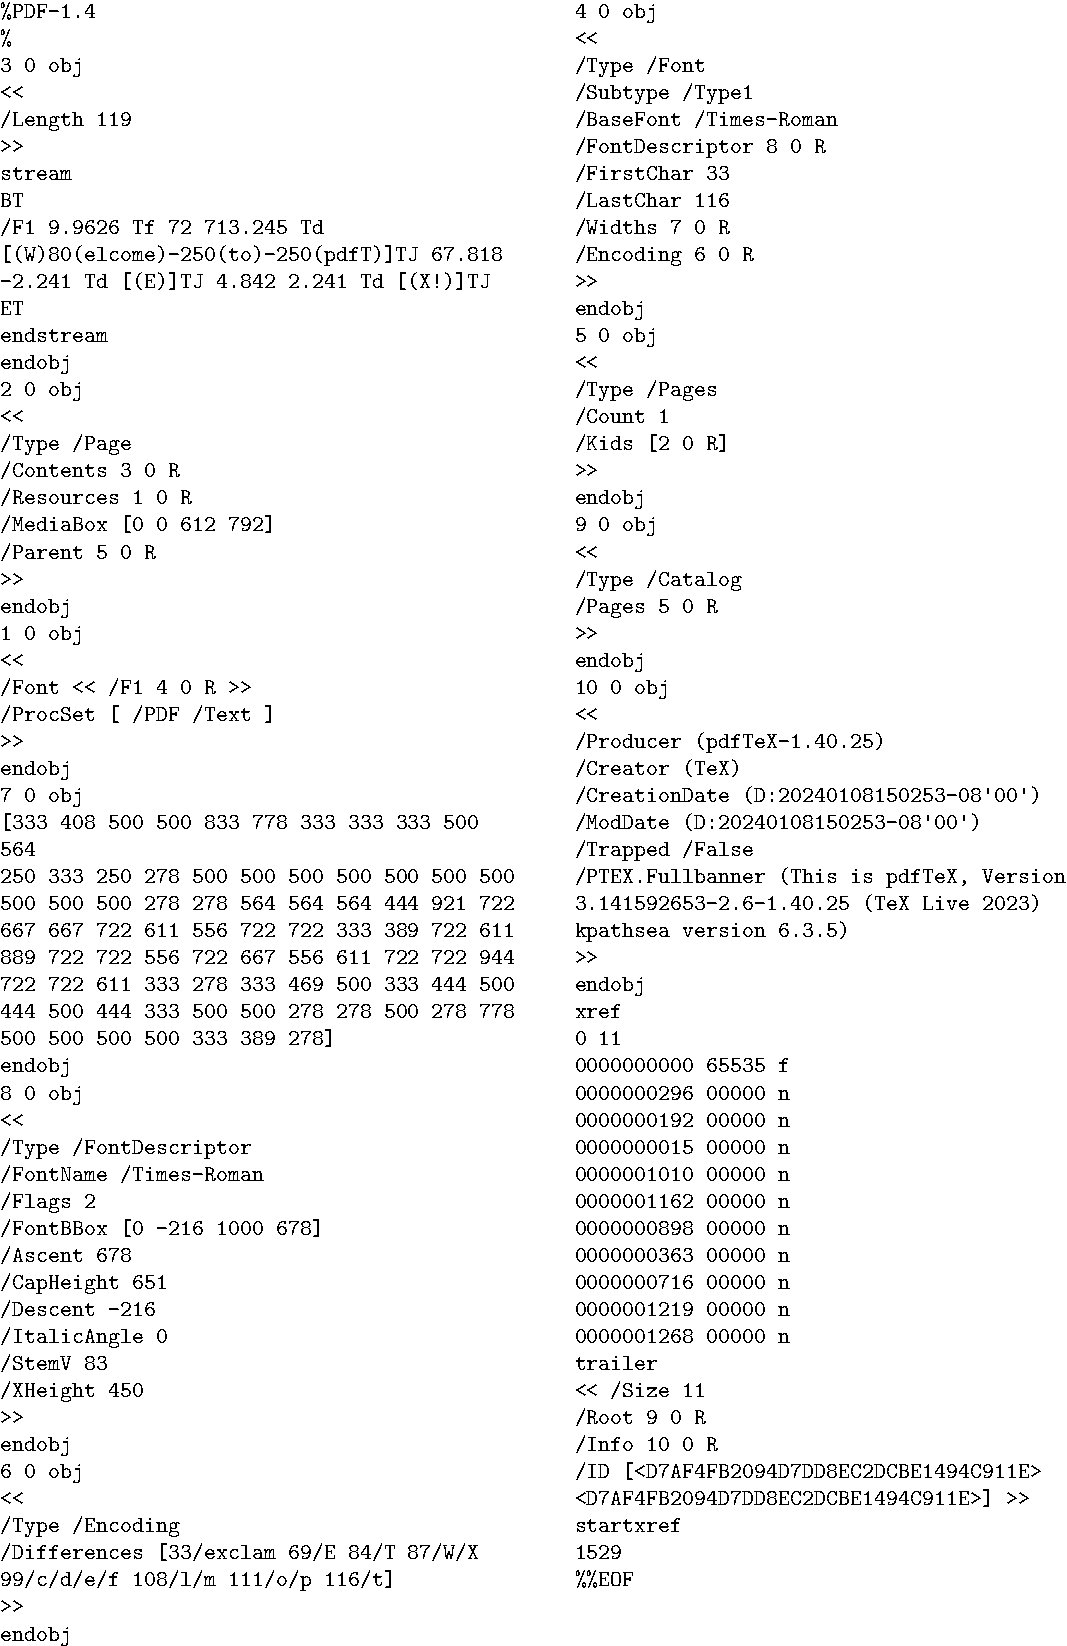
\includegraphics[height=1.27\vsize,alt={small PDF file}]
                      {incl/pdfmin-crop.pdf}
\caption{The \PDF\ output for the \TeX\ source in figure~\ref{fig.titlesource}.}
\label{fig.titleout}
\end{figure}

A \PDF\ file consists of objects. These objects can be recognized by their
number and keywords. For example, over in the second column, we can see
(modulo editorial line breaks):

\begin{verbatim}
9 0 obj << /Type /Catalog /Pages 5 0 R >> endobj
\end{verbatim}

Here \verb|9 0 obj ... endobj| is the object capsule. The first number
is the object number (no.~9). The sequence \verb|5 0 R| is an object
reference, that is, a pointer to another object (no.~5). The second
number (here a zero) is currently not used in \PDFTEX; it is the version
number of the object. It is, for instance, used by \PDF\ editors, when
they replace objects by new ones.

When a viewer opens a \PDF\ file, it goes to the end of the file,
looking for the keyword \type{startxref}. The number after
\type{startxref} gives the absolute position (byte offset from the file
start) of the so\hyph called ``object cross-reference table'' that
begins with the keyword \type{xref}. This table in turn tells the byte
offsets of all objects that make up the \PDF\ file, providing fast
random access to the individual objects (here the \type{xref} table
shows 11~objects, numbered from~0 to~10; object no.~0 is always unused).
The actual starting point of the file's object structure is defined
after the \type{trailer}: the \type{/Root} entry points to the
\type{/Catalog} object (no.~9). In this object the viewer can find the
pointer \type{/Pages} to the page list object (no.~5). In our example we
have only one page. The trailer also usually holds an \type{/Info}
entry, which points to an object (no.~10) with a bit more about the
document. We can follow the thread:

\begin{quote}
\type{/Root}     $\longrightarrow$ object~9 $\longrightarrow$
\type{/Pages}    $\longrightarrow$ object~5 $\longrightarrow$
\type{/Kids}     $\longrightarrow$ object~2 $\longrightarrow$
\type{/Contents} $\longrightarrow$ object~3
\end{quote}

As soon as we add annotations, a fancy word for hyperlinks and the like,
some more entries will be present in the catalog. We invite users to
take a look at the \PDF\ code of this file to get an impression of that.

The page content is a stream of drawing operations. Such a stream can be
compressed, where the level of compression can be set with
\cs{pdfcompresslevel} (compression is switched off for the title page).
Let's take a closer look at this stream in object~3. Often (but not in
our example) there is a transformation matrix, six numbers followed by
\type{cm}. As in \POSTSCRIPT, the operator comes after the operands.
Between \type{BT} and \type{ET} comes the text. A font is selected by a
\type{Tf} operator, which is given a font resource name \type{/F..} and
the font size. The actual text goes into parentheses \type{()} so that
it creates a \POSTSCRIPT\ string. The numbers in bracket pairs provide
horizontal movements like spaces and fine glyph positioning (kerning).
When one analyzes a file produced by a less sophisticated typesetting
engine, whole sequences of words can be recognized. In \PDF\ files
generated by \PDFTEX\ however, many words come out rather fragmented,
mainly because a lot of kerning takes place; in our example the
\type{80} moves the text \type{(elcome)} left towards the letter
\type{(W)} by 80/1000 of the font size. \PDF\ viewers in search mode
simply ignore the kerning information in these text streams. When a
document is searched, the search engine reconstructs the text from these
(string) snippets.

Every \type{/Page} object points also to a \type{/Resources} object
(no.~1) that gives all ingredients needed to assemble the page. In our
example only a \type{/Font} object (no.~4) is referenced, which in turn
tells that the text is typeset in \type{/Font} \type{/Times-Roman}. The
\type{/Font} object points also to a \type{/Widths} array (object no.~7)
that tells for each character by how much the viewer must move forward
horizontally after typesetting a glyph.

More details about the font can be found in the \type{/FontDescriptor}
object (no.~8); if a font file is embedded, this object points to the
font program stream. But as the Times-Roman font used for our example is
one of the 14 so\hyph called standard fonts that should always be present in
any \PDF\ viewer and therefore need not be embedded in the \PDF\ file,
it is left out here for brevity. However, when we use for instance a
Computer Modern Roman font, we have to make sure that this font is later
available to the \PDF\ viewer, and the best way to do this is to embed
the font. It's highly recommended nowadays to embed even the standard
fonts; you can't know how it looks exactly at the viewer side unless you
embed every font.

In this simple file we don't specify in what way the file should be
opened, for instance full screen or clipped. A closer look at the page
object no.~2 (\type{/Type/Page}) shows that a mediabox
(\type{/MediaBox}) is part of the page description. A mediabox acts like
the (high-resolution) bounding box in a \POSTSCRIPT\ file. \PDFTEX\
users can add dictionary entries to page objects with the
\cs{pdfpageattr} primitive.

Although in most cases macro packages will shield users from these
internals, \PDFTEX\ provides access to many of the entries described
here, either automatically by translating the \TEX\ data structures into
\PDF\ ones, or manually by pushing entries to the catalog, page, info or
self-created objects. One can for instance create an object by using
\cs{pdfobj}, after which \cs{pdflastobj} returns its number. So

\begin{verbatim}
\pdfobj { << /Type/ExtGState /LW 2 >> }
\end{verbatim}

\noindent inserts an object into the \PDF\ file (it creates a ``graphics
state'' object setting the line width to 2~units), and \cs{pdflastobj}
now returns the number \PDFTEX\ assigned to this object. Unless objects
are referenced by others, they will just end up as isolated entities,
not doing any real harm but bloating the \PDF\ file.

In general this rather direct way of pushing objects in the \PDF\ files
by primitives like \cs{pdfobj} is not very useful, and only makes
sense when implementing, say, fill\hyph in field support or annotation
content reuse. We will come to that later.

Of course, this is just the barest introduction to \PDF\ format. For
those who want to learn more about technical \PDF\ details, the best bet
is to read the \PDFReference\ (\useurl{pdfreference}).

We turn now to the specifics of \PDFTEX.

\chapter{Invoking \PDFTEX}

\PDFTEX\ has many command line options and can use many environment
variables and configuration file settings. Except for the simple and
rarely-used \type{-draftmode} and \type{-output-format} options, they
are all inherited from the common framework for \TeX\ engines as
implemented in \WEBC\ and Kpathsea. Their documentation is available at
\useurl{webc} and \useurl{kpathsea}.

Two additional environment variables need more description here: first,
\type{SOURCE_DATE_EPOCH} (introduced in version 1.40.17, 2016). If this
is set, it must be a positive integer (with one trivial exception: if it
is set but empty, that is equivalent to 0). Non-integer values cause a
fatal error. The value is used as the current time in seconds since the
usual Unix ``epoch'': the beginning of 1970-01-01, UTC. Thus, a value of
\type{32} would result in a \type{/CreationDate} and \type{/ModDate}
values of \type{19700101000032Z}. This is useful for reproducible builds
of documents. (See also \cs{pdfinfoomitdate}, \cs{pdfsuppressptexinfo},
et al.)

The second, related, environment variable is \type{FORCE_SOURCE_DATE}.
If this is set to~\type{1}, \TEX's time-related primitives are also
initialized from the value of \type{SOURCE_DATE_EPOCH}. These primitives
are \cs{year}, \cs{month}, \cs{day}, and \cs{time}. If
\type{SOURCE_DATE_EPOCH} is not set, setting \type{FORCE_SOURCE_DATE}
has no effect. If \type{FORCE_SOURCE_DATE} is unset, set to the empty
string, or set to~\type{0}, the primitives reflect the current time as
usual. Any other value elicits a warning, and the current time is used.
This is useful if one wants to make reproducible \PDF{}s for a set
of documents without changing them in any way, \eg\ an operating system
distribution with manuals that use \cs{today}. Except in such unusual
circumstances, it is better not to set this, and let the \TEX\
primitives retain the meaning they have always had.

In addition, if both \type{SOURCE_DATE_EPOCH} and
\type{FORCE_SOURCE_DATE} are set, \cs{pdffilemoddate} returns a value
in UTC, ending in \type{Z}. (The values of the environment variables are
irrelevant in this case.)

Finally, just to have the list of options and basic invocation at hand,
here is a verbatim listing of the \type{--help} and \type{--version}
output. All options can be specified with one or two dashes and
unambiguously abbreviated.

\myverbatiminput{incl/pdftex-help.txt}

\section{Macro packages supporting \PDFTEX}

Currently all mainstream macro packages offer \PDFTEX\ support, with
automatic detection of \PDFTEX\ as engine. So there is normally no need
to turn on \PDFTEX\ support explicitly.

\begin{itemize}
\item  For \LATEX\ users, the \type {hyperref} package (originally
       written by Sebastian Rahtz and Heiko Oberdiek; now maintained by
       the \LaTeX\ team, has substantial support for \PDFTEX\ and
       provides access to most of its features. In the simplest and most
       common case, the user merely needs to load \type{hyperref}, and
       all cross\hyph references will be converted to \PDF\ hypertext
       links. \PDF\ output is automatically selected, compression is
       turned on, and the \PDF\ page size is set up correctly. Bookmarks
       are created to match the table of contents.

\item  The standard \LATEX\ packages \type{graphics}, \type{graphicx}, and
       \type{color} also have built-in \PDFTEX\ support, which allows
       use of color, text rotation, and graphics inclusion commands.

\item  The \CONTEXT\ MkII system by Hans Hagen has full support
       for \PDFTEX\ in its generalized hypertext features.
       The latest \CONTEXT\ supports advanced \PDF\ output, but
       uses a engine (\LMTX).

\item  \PDF\ from \GNU\ \TEXINFO\ documents can be created by running
       \PDFTEX\ on the \TEXINFO\ file, instead of \TEX. Alternatively,
       run the shell command \type{texi2pdf} instead of \type{texi2dvi}.

\item  For plain \TEX\ users, the \filename{miniltx.tex} file from the
       \type{graphics-pln} package allows loading \type{graphics},
       \type{graphicx}, and \type{color}. \EPLAIN\ provides additional
       support for hyperlinks.

\item  A modification of \filename {webmac.tex}, named \filename
       {pdfwebmac.tex}, allows production of hyperlinked \PDF\ versions
       of the literate source code written in \WEB, such as \PDFTEX.

\end{itemize}

For \TeX\ developers: as \PDFTEX\ generates the final \PDF\ output
without help of a postprocessor, macro packages that take care of these
\PDF\ features have to be set up properly. Tasks include handling color,
graphics, hyperlink support, threading, fonts, page imposition and
manipulation. All of these \PDF\hyph specific tasks can be controlled by
\PDFTEX's own primitives (a few also by a \PDFTEX\hyph specific
\verb|\special{pdf: ...}|). Any other \cs{special} commands, like the
ones defined for various \DVI\ postprocessors, are simply ignored by
\PDFTEX\ when in \PDF\ output mode; a warning is given for non\hyph
empty \cs{special} commands.

When a macro package written for classical \TEX\ with \DVI\ output is to
be modified for use with \PDFTEX, it is helpful to get some insight to
what extent \PDFTEX\hyph specific support is needed. This info can be
gathered, for instance, by outputting the various \cs{special} commands
via \cs{message}. as in:

\begin{verbatim}
\pdfoutput=1 \let\special\message
\end{verbatim}

or, if this leads to confusion,

\begin{verbatim}
\pdfoutput=1 \def\special#1{\write16{special: #1}}
\end{verbatim}

and see what happens. As soon as one \type{special:} message turns up,
one knows for sure that some kind of \PDFTEX\hyph specific support is
needed, and often the message itself gives a indication of what is
needed.

\chapter{Setting up fonts}

\PDFTEX\ can work with Type~1 and TrueType fonts (and to a small extent
also with OpenType fonts). Font files should be available and embedded
for all fonts used in the generated \PDF. It is possible to use
\METAFONT\hyph generated fonts in \PDFTEX---but it is strongly
recommended not to use these fonts if an equivalent is available in
Type~1 or TrueType format, if only because bitmap Type~3 fonts render
poorly under enlargement.

\section{Map files}
\label{sec.mapfile}

Font map files provide the connection between \TEX\ \TFM\ font files
and outline font file names. They contain also information about
re\hyph encoding arrays, partial font embedding (``subsetting''), and
character transformation parameters (like SlantFont and ExtendFont). Those
map files were first created for \DVI\ postprocessors. But, as \PDFTEX\
in \PDF\ output mode includes all \PDF\ processing steps, it also needs
to know about font mapping, and therefore reads in one or more map files.
Map files are not read in when \PDFTEX\ is in \DVI\ mode. Bitmap fonts
can (and normally should) be used without being listed in the map file.

By default, \PDFTEX\ reads the map file \filename{pdftex.map}.  In \WEBC,
map files are searched for using the \type{TEXFONTMAPS} config file value
and environment variable.  By default, the current directory and various
system directories are searched.

Within the map file, each font is listed on a single line.  The syntax of
each line is upward\hyph compatible with \type{dvips} map files and can contain
the following fields (some are optional; explanations follow):

\begin{quote}
\varname{tfmname psname fontflags special encodingfile fontfile}
\end{quote}

Here are two (real-world) examples. All the values are explained in
detail in the following.

{\small \begin{verbatim}
cmr10 CMR10 <cmr10.pfb
ptmr8y NimbusRomNo9L-Regu " TeXnANSIEncoding ReEncodeFont " <texnansi.enc <utmr8a.pfb
\end{verbatim}
\par % needed for tagging; alternative: \begin{small}...\end{small}
     % another alternative: \AddToHookNext{env/verbatim/begin}{\small}
}

It is mandatory that \varname{tfmname} is the first field. If a
\varname{psname} is given, it must be the second field. Similarly if
\varname{fontflags} is given it must be the third field (if
\varname{psname} is present) or the second field (if \varname{psname} is
left out). The positions of \varname{special}, \varname{encodingfile},
and \varname{fontfile} can be mixed.

\subsection{Map lines: \varname{tfmname}}
\label{sec.map-tfmname}

The \varname{tfmname} field specifies the name of the \TFM\ file for a
font---the file name given in a \TEX\ \cs{font} command. This name must
always be given, with no extension. Examples: \type{cmr10},
\type{ptmr8y}.

\subsection{Map lines: \varname{psname}}

The \varname{psname} field specifies the \POSTSCRIPT\ (or other outline)
font name, as defined within the outline font file. Examples:
\type{CMR10}, \type{NimbusRomNo9L-Regu}. It is highly recommended to use
the \varname{psname} field, but strictly speaking it is optional. It has
two main uses.

First, when a \PDF\ file is embedded by \cs{pdfximage}, the
\type{/BaseFont} names in the font dictionaries of Type~1 and Type~1C
(CFF) fonts from the embedded \PDF\ file are checked against this {\em
psname} field. If names match, the glyphs of that font will not be
copied from the embedded \PDF\ file, but instead a local font is opened,
and all needed glyphs will be taken from the Type~1 font file that is
mentioned in the map line (see \varname{fontfile} below). By this
collecting mechanism Type~1 glyphs can be shared between several
embedded \PDF\ files and with text that is typeset by \PDFTEX, which
helps keep the resulting \PDF\ file size smaller, if many files with
similar Type~1(C) fonts are embedded. Replacing Type~1 fonts from
embedded \PDF\ files requires that also a Type~1 font file name is in
the \varname{fontfile} field (see below).

Second, if a font file is not to be embedded into the \PDF\ output
(\varname{fontfile} field missing), then the \varname{psname} field will
be copied to the \type{/BaseFont} and \type{/FontName} dictionary
entries in the \PDF\ file, so that the \POSTSCRIPT\ font name will be
known to viewers and other \PDF-reading applications.

\subsection{Map lines: \emph{fontflags}}

The \emph{fontflags} field optionally specifies various characteristics
of the font. The following description of these flags is taken, with
slight modification, from the \PDFReference\ (the section on font
descriptor flags). Viewers may adapt their rendering to these flags,
especially when they substitute for a non-embedded font.

The value of the flags key in a font descriptor is a 32-bit integer that
contains a collection of boolean attributes. These attributes are true
if the corresponding bit is set to~1. The following table specifies the
meanings of the bits, with bit~1 being the least significant. Reserved
bits must be set to zero.

\begin{smalltable}
\begin{tabular}{cl}
\bf bit position & \bf semantics                               \cr
1                & Fixed-width font                            \cr
2                & Serif font                                  \cr
3                & Symbolic font                               \cr
4                & Script font                                 \cr
5                & Reserved                                    \cr
6                & Uses the Adobe Standard Roman character set \cr
7                & Italic                                      \cr
8--16            & Reserved                                    \cr
17               & All-capitals font                           \cr
18               & Small-capitals font                         \cr
19               & Force bold at small text sizes              \cr
20--32           & Reserved                                    \cr
\end{tabular}
\end{smalltable}

The first several bits specify the general type of font. All characters
in a \emph{fixed-width} font (a.k.a.\ monospaced, typewriter) have the
same width, while characters in a proportional font have different
widths. Characters in a \emph{serif font} have short strokes drawn at an
angle on the top and bottom of character stems, while sans serif fonts
do not have such strokes. A \emph{symbolic font} contains symbols rather
than letters and numbers. Characters in a \emph{script font} resemble
cursive handwriting. An \emph{all-capitals} font, which is typically
used for display purposes such as titles or headlines, contains no
lowercase letters. It differs from a \emph{small-capitals} font in that
characters in the latter, while also capital letters, have been sized
and their proportions adjusted so that they have the same size and
stroke weight as lowercase characters in the same typeface family.

Bit~6 in the flags field indicates that the font's character set
conforms to the Adobe Standard Roman Character Set, or a subset of that,
and that it uses the standard names for those characters.

Finally, bit~19 is used to determine whether or not bold characters are
drawn with extra pixels even at very small text sizes. Typically, when
characters are drawn at small sizes on very low resolution devices such
as display screens, features of bold characters may appear only one pixel
wide. Because this is the minimum feature width on a pixel\hyph based device,
ordinary non\hyph bold characters also appear with one\hyph pixel wide features,
and thus cannot be distinguished from bold characters. If bit~19 is set,
features of bold characters may be thickened at small text sizes.

If the \varname{fontflags} field is not given, and the font is embedded,
\PDFTEX\ treats it as the value~4 (decimal, that is, bit position 3 is
set), a symbolic font. For non-embedded fonts, the default value is
\type{0x22}, a non-symbolic serif font. If you do not know the correct
value, it is best not to specify it at all, as specifying a bad value of
font flags may cause trouble in viewers. On the other hand this option
is not absolutely useless because it provides backward compatibility
with older map files (see the \varname{fontfile} description below).

\subsection{Map lines: \varname{special}}

The \varname{special} field specifies font manipulations in the same way
as \type{dvips}. Currently only the keywords \type{SlantFont} and
\type{ExtendFont} are interpreted; other instructions (notably
\type{ReEncodeFont} and its parameters, see \varname{encoding} below)
are ignored. The permitted \type{SlantFont} range is $-1..1$; for
\type{ExtendFont} it's $-2..2$. The text of the \varname{special} field
must be enclosed by ASCII double quote characters: \type{"}.

\subsection{Map lines: \varname{encodingfile}}

The \varname{encodingfile} field specifies the name of the file
containing the external encoding vector to be used for the font. The
encoding file name must have the extension \type{.enc}, and the file
name including extension must be given with either a preceding~\type{<}
character or a preceding~\type{<[}. The format of the encoding vector is
identical to that used by \type{dvips}. If no encoding is specified, the
font's built\hyph in default encoding is used. The
\varname{encodingfile} field may be omitted if you are sure that the
font resource has the correct built-in encoding. In general this option
is highly recommended, and it is required when subsetting a TrueType
font.

Starting with \PDFTEX\ version 1.40.19, an encoding file can also be
specified for bitmap \PK\ fonts. In this case, it assigns the glyph
names from the given encoding vector, which can be used with the
\cs{pdfglyphtounicode} primitive (q.v.). For example:

\begin{verbatim}
\pdfglyphtounicode{ffi}{0066 0066 0069} % normally: \input glyphtounicode
\pdfgentounicode=1
\pdfmapline{cmb10 <7t.enc}
\font\cmb=cmb10 \cmb ffi
\end{verbatim}

The result is a \PDF\ file with a correctly-labeled \type{/ffi}
character instead of the numeric character position in \type{cmb10.tfm}
(decimal 14).

\subsection{Map lines: \varname{fontfile}}

The \varname{fontfile} field sets the name of the font file to be
embedded into the \PDF\ output for a given \TeX\ font; the
\varname{tfmname}~$\leftrightarrow$~\varname{fontfile} mapping is the
most prominent use of the \filename{pdftex.map} file.

The font file name must refer to a Type~1 or TrueType font file. If the
\varname{fontfile} field is missing, no font embedding can take place; a
warning will be given, unless the \varname{psname} field contain one of
the 14 standard font names. Not embedding all fonts in a \PDF\ file is
troublesome, as this forces the \PDF\ viewer to use or synthesize a
replacement, typically with awful results.

The font file name should be preceded by one or two special characters,
specifying how to handle the font file:

\begin{itemize}
\item  If the font file name is preceded by a \type{<} character
       (as in \type{<cmr10.pfb}), the font file will be only partially
       embedded in the \PDF\ output (``subsetted''), meaning that only
       used glyphs are written to the \PDF\ file. This is the most
       common use and is \emph{strongly recommended} for any font, as it
       ensures the portability and reduces the size of the \PDF\ output.
       Subsetted fonts are included in such a way that name and cache
       clashes are minimized.

\item  If the font file name is preceded by a double \type{<<}, the font
       file will be included entirely---all glyphs of the font are
       embedded, including even those not used in the document. Apart
       from increasing the \PDF\ output size, this option may cause
       troubles with TrueType fonts, so it is normally not recommended
       for Type~1 or TrueType fonts. But this is currently the only mode
       that allows the use of OpenType fonts. This mode might also be
       useful in case the font is atypical and cannot be subsetted well
       by \PDFTEX. {\em Beware: proprietary font vendors typically
       forbid full font inclusion.}

\item  As of \PDFTEX\ version 1.40.0, if no special character precedes
       the font file name, it is ignored, with a warning. You achieve
       exactly the same \PDF\ result if you just remove the font file
       name from the map entry. Then the glyph widths that go into the
       \PDF~file are extracted from the \TFM~file, and a font descriptor
       object is created that contains approximations of the font
       metrics for the selected font.

\item  Specifying the {\em psname} and no font file name is only useful
       as a last-ditch fallback when you do not want to embed the font
       (\eg\ due to font license restrictions), but wish to use the font
       metrics and let the \PDF\ viewer generate instances that look
       close to the used font, in case the font resource is not
       installed on the system where the \PDF\ output will be viewed or
       printed. To use this feature, the font flags {\em must} be
       specified, and it must have the bit~6 set on, which means that
       only fonts with the Adobe Standard Roman character set can be
       simulated. The only exception is the case of a symbolic font.
       In these days of Unicode, these font approximations are not
       likely to be useful.
\end{itemize}

If you encounter problematic lookups, for instance if \PDFTEX\ tries
to open a \type{.pfa} file instead of a \type{.pfb}, you can add
the suffix to the filename.  In this respect, \PDFTEX\ completely relies
on the Kpathsea library.

For Type~1 and TrueType fonts, the font file will be included only once
in the \PDF\ output, regardless of how many \TeX\ \cs{font} instances
are used in the document. For instance, given

\begin{verbatim}
\font\a = cmr12
\font\b = cmr12 at 11pt
\end{verbatim}

the outline file \type{cmr12.pfb} will only be included once in the
\PDF, and merely scaled down to create the instance for \cs{b}.

If a used font is not present in the map files, \PDFTEX\ will try to use
\PK~fonts as most \DVI\ drivers do, creating \PK~fonts on-the-fly if
needed. This is the normal, and recommended, way to use bitmap fonts.

\subsection{Map lines: summary}

To summarize this rather complex story, let's look at some more example
map lines. The most common way is to embed only a subset of glyphs from
a font for a particular desired encoding, here~\type{8r}:

\begin{verbatim}
ptmri8r Times-Italic <8r.enc <ptmri8a.pfb
\end{verbatim}

Without re-encoding it looks like this:

\begin{verbatim}
cmr10 CMR10 <cmr10.pfb
\end{verbatim}

\type{SlantFont} and \type{ExtendFont} fields are specified as with
\type{dvips}:

\begin{verbatim}
psyro   StandardSymL ".167 SlantFont"         <usyr.pfb
pcrr8rn Courier      ".85 ExtendFont" <8r.enc <pcrr8a.pfb
\end{verbatim}

Entirely embed a font into the \PDF\ file without and with re-encoding
(not typically useful):

\begin{verbatim}
fmvr8x MarVoSym         <<marvosym.pfb
pgsr8r GillSans <8r.enc <<pgsr8a.pfb
\end{verbatim}

A TrueType font can be used in the same way as a Type~1 font:

\begin{verbatim}
verdana8r Verdana <8r.enc <verdana.ttf
\end{verbatim}

Finally, a few cases with non-embedded fonts. If the font file is
missing, the viewer application will have to use its own approximation
of the missing font (with and without re-encoding):

\begin{verbatim}
ptmr8r Times-Roman <8r.enc
psyr Symbol
\end{verbatim}

In the final example the numerical font flags (bit position 6) specify
using the Adobe Standard Roman character set, so the viewer might try an
approximation:

\begin{verbatim}
pgsr8r GillSans 32
\end{verbatim}

Not embedding fonts is rather risky and should generally be avoided. The
recommendation these days is to embed all fonts, even the 14 standard
ones.

\section{Helper tools for TrueType fonts: \texttt{ttf2afm}}

As mentioned above, \PDFTEX\ can work with TrueType fonts. Defining
TrueType fonts is similar to Type~1. The only extra thing to do with
TrueType is to create a \TFM\ file. There is a program called
\type{ttf2afm} in the \PDFTEX\ distribution which can be used to extract
\AFM\ from TrueType fonts (another conversion program is
\type{ttf2pt1}). Basic usage of \type{ttf2afm}:

\begin{verbatim}
ttf2afm -e encfile.enc -o output.afm input.ttf
\end{verbatim}

A TrueType file can be recognized by its suffix \filename{ttf}.
If no \type{-o} option is given, \type{ttf2afm} writes the output \AFM\
to standard output. 

The optional \varname{encfile} specifies the encoding, which is the same
as the encoding vector used in map files for \PDFTEX\ and \type{dvips}.
That is, it must be an 8-bit encoding, not Unicode. If the encoding is
not given, all the glyphs of the \AFM\ output will be mapped to
\type{/.notdef}. If we need to know which glyphs are available in the
font, we can run \type{ttf2afm} without any \type{-e} to get all glyph
names. The resulting \AFM\ file can be used to generate a \TFM\ by
applying the \filename {afm2tfm} utility.

To use a new TrueType font the minimal steps may look like below, supposing
that a map file \filename {test.map} is used.

\begin{verbatim}
ttf2afm -e 8r.enc -o times.afm times.ttf
afm2tfm times.afm -T 8r.enc
echo "times TimesNewRomanPSMT <8r.enc <times.ttf" >>test.map
\end{verbatim}

There are a limitations with TrueType fonts in comparison with
Type~1 fonts:

\begin{itemize}
\item  The special effects SlantFont\slash ExtendFont did not work
       before version 1.40.0.
\item  To subset a TrueType font, the font must be specified as re\hyph
       encoded, therefore an encoding vector must be given.
\item  TrueType fonts used in embedded \PDF\ files are kept
       untouched; they are not replaced or merged with the same font
       used in the document, as happens with Type~1.
\end{itemize}

For much more about \PDFTEX\ and TrueType fonts, including many details
on handling glyph names, see ``A closer look at TrueType fonts and
\PDFTEX'', \titleref{TUGboat} 30:1 (2009), pp.~32\hyph 34,
\useurl{thanhtruetypetub}.

\chapter{\PDFTEX\ primitives}
\label{sec.primitives}

Here follows a description of the primitives added by \PDFTEX\ to the
original \TEX\ engine (other extensions by \ETEX, \MLTEX\ and \ENCTEX\
are not described). Many of these primitives are described further in
the \filename {samplepdf.tex} file in the \PDFTEX\ distribution (q.v.).

If the output is \DVI, then the \PDFTEX-specific dimension parameters
are not used at all. However, some \PDFTEX\ integer parameters can
affect \DVI\ as well as \PDF\ output (specifically, \cs{pdfoutput} and
\cs{pdfadjustspacing}).

A warning to macro writers: if you define macros whose names start with
\cs{pdf}, you risk name clashes with new primitives that may be
introduced in future versions of \PDFTEX.

General warning: many of these new primitives, for example \cs{pdfdest}
and \cs{pdfoutline}, write their arguments directly to the \PDF\ output
file (when producing \PDF), as \PDF\ string constants. This means that
\emph{you} (or, more likely, the macros you write) must escape
characters as necessary (namely \cs{}, \type{(}, and \type{)}.
Otherwise, an invalid \PDF\ file may result. The \type{hyperref} and
\TEXINFO\ packages have code which may serve as a starting point for
implementing this, although it will certainly need to be adapted to any
particular situation.

\section{Document setup}

\subsection{\cs{pdfoutput}}
\pdftexprimitive{\Syntax{\cs{pdfoutput} \Whatever{integer}}}

This parameter specifies whether the output format should be \DVI\ or
\PDF. A positive value means \PDF\ output, otherwise (default 0) one
gets \DVI\ output. This primitive is the only one that must be set to
produce \PDF\ output (the command-line option \type{-output-format=pdf}
may alternatively be used); all other primitives are optional. This
parameter cannot be specified \emph{after} shipping out the first page.
In other words, to get \PDF\ output, we have to set \cs{pdfoutput}
before \PDFTEX\ the first page.

A simple way of making macros aware of \PDFTEX\ in both \PDF\ or \DVI\
mode is:

\begin{verbatim}
\ifx\pdfoutput\undefined \csname newcount\endcsname\pdfoutput \fi
\ifcase\pdfoutput DVI CODE \else PDF CODE \fi
\end{verbatim}

Using the \type{ifpdf.sty} file, which works with both \LATEX\ and plain
\TeX, is a cleaner way of doing this. Originally, the simple test
\verb|\ifx\pdfoutput\undefined| sufficed; but for many years, the
\PDFTEX\ engine is used in distributions also for non-\PDF\ formats
(\eg\ \LATEX), so \cs{pdfoutput} may be defined even when the output
format is \DVI.

\subsection{\cs{pdfmajorversion}, \cs{pdfminorversion}}
\pdftexprimitive{\Syntax{\cs{pdfmajorversion} \Whatever{integer}}}
\pdftexprimitive{\Syntax{\cs{pdfminorversion} \Whatever{integer}}}

Together, these two primitives specify the \PDF\ version for generated \PDF\
output. The defaults compiled into the \PDFTEX\ program are
\cs{pdfmajorversion=1} and \cs{pdfminorversion=4}, thus \PDF~1.4
is generated by default.

However, distributions typically alter the engine's compiled default
minor version of~4 when building formats. For example, as of 2010,
\TEXLIVE\ sets \cs{pdfminorversion=5} when formats are built. This is
so object compression can be enabled (see \cs{pdfobjcompress} below).

This value also defines the highest \PDF\ version for included \PDF{}s
to be allowed without error, by default (see
\cs{pdfinclusionerrorlevel}).

The values for both must be $\ge1$ but are not checked further.
Furthermore, they are set independently; setting only 
\cs{pdfmajorversion=2} would result in \PDF~2.4 output; it's
necessary to additionally set \cs{pdfminorversion}.

If specified, these primitives must appear before any data is written to
the generated \PDF\ file. The \cs{pdfmajorversion} primitive was
introduced in \PDFTEX\ 1.40.21. \cs{pdfminorversion} was originally a
synonym of the \cs{pdfoptionpdfminorversion} command, which is now
obsolete. \introduced{1.30.0}

\subsection{\cs{pdfcompresslevel}}
\pdftexprimitive{\Syntax{\cs{pdfcompresslevel} \Whatever{integer}}}

This integer parameter specifies the level of stream compression. Zero
means no compression, 1~means fastest, 9~means best, $2..8$ means
something in between. A value outside this range will be adjusted to the
nearest meaningful value. This parameter is read each time \PDFTEX\
starts a stream.

This compression applies to text, inline graphics, and embedded \PNG\
images (but only if they are un- and re-compressed during the embedding
process). It is implemented by the \type{zlib} library).

Setting \cs{pdfcompresslevel=0} is useful for \PDF\ stream debugging.

\subsection{\cs{pdfobjcompresslevel}}
\pdftexprimitive{\Syntax{\cs{pdfobjcompresslevel} \Whatever{integer}}}

This integer parameter controls the compression of non-stream objects.
If specified, the parameter must appear before any data is written to
the \PDF\ output. \introduced{1.40.0}

In the \PDF-1.4 specification, non-stream objects had to be written in
the \PDF\ file as clear text, uncompressed. The \PDF-1.5 specification
allows collecting non-stream objects as ``compressed objects'' into
``object stream'' objects (\type{/Type/ObjStm}, see the \PDFReference,
5th~ed., \S3.4.6). At the end of the \PDF\ file, an \type{/XRef}
cross-reference stream is then written out instead of the object table.
This can result in a considerably smaller \PDF\ file, particularly if
lots of annotations and links are used.

The writing of compressed objects is enabled by setting
\cs{pdfobjcompresslevel} to a value between~1 and~3; it's disabled if~0
(default). Object compression also requires
$\cs{pdfminorversion}\ge5$ (or $\cs{pdfmajorversion}\ge2$), else
a warning is given and the compression is disabled. The value of
\cs{pdfobjcompresslevel} is clipped to the range $0..3$, but using
values outside this range is not recommended (for future extension).

Values for \cs{pdfobjcompresslevel} have the following effects:

\begin{itemize}
\item When set to~0, no object streams are generated at all.

\item When set to~1,
all non-stream objects are compressed with the exception of any objects
coming with embedded \PDF\ files (``paranoid'' mode, to avoid yet unknown
problems), and also the \type{/Info} dictionary is not compressed for
clear-text legibility.

\item When set to~2, also all non-stream objects coming
with embedded \PDF\ files are compressed, but the \type{/Info} dictionary
is still not compressed.

\item Finally, when set to~3, all non-stream objects
are compressed, including the \type{/Info} dictionary (this means that
the \type{/Info} can't be read as clear text any more). If object streams
are to be used, currently \cs{pdfobjcompresslevel=2} is recommended,
and is so specified in some distributions, including \TEXLIVE~2010 and later.
\end{itemize}

\emph{Compatibility caveats:} \PDF\ files generated with object
streams enabled can't be read with (sufficiently old) \PDF\ viewers that
don't understand \PDF-1.5 files. For widest distribution and unknown
audience, don't activate object stream writing. The \PDF-1.5 standard
describes also a hybrid object compression mode that gives some backward
compatibility, but this is currently not implemented, as \PDF-1.5 was
rather quickly adopted by modern \PDF\ viewers. Also not implemented is
the optional \type{/Extends} key.

\subsection{\cs{pdfdecimaldigits}}
\pdftexprimitive{\Syntax{\cs{pdfdecimaldigits} \Whatever{integer}}}

This integer parameter specifies the numeric accuracy of real
coordinates as written to the \PDF\ file. It gives the maximal number of
decimal digits after the decimal point. Valid values are in the range
$0..4$. A higher value means more precise output, but also results in a
larger file size and more time to display or print. In most cases the
optimal value is~2. This parameter does not influence the precision of
numbers used in raw \PDF\ code, like that used in \cs{pdfliteral} and
annotation action specifications; also multiplication items (\eg\
scaling factors) are not affected and are always output with best
precision.  This parameter is read when \PDFTEX\ writes a real number to
the \PDF\ output.

When including huge \METAPOST\ images using \filename {supp-pdf.tex}, one can
limit the accuracy to two digits with \cs{twodigitMPoutput}.

\subsection{\cs{pdfhorigin}}
\pdftexprimitive{\Syntax{\cs{pdfhorigin} \Whatever{dimen}}}

This parameter can be used to set the horizontal offset of the output
box from the top left corner of the page. A value of 1~inch corresponds
to the normal \TEX\ offset. This parameter is read when \PDFTEX\ starts
shipping out a page to the \PDF\ output.

For all normal purposes, this parameter should always be kept at 1~true
inch. If you want to shift text on the page, use \TEX's own \cs{hoffset}
primitive. To avoid surprises, after global magnification has been
changed by the \cs{mag} primitive, the \cs{pdfhorigin} parameter should
still be 1~true inch, \eg\ by setting \cs{pdfhorigin=1 true in} after
the \cs{mag} setting. Or, you can preadjust the \cs{pdfhorigin} value
before typing \cs{mag}, so that its value after the \cs{mag} command
ends up at 1~true inch again.

\subsection{\cs{pdfvorigin}}
\pdftexprimitive{\Syntax{\cs{pdfvorigin} \Whatever{dimen}}}

This parameter is the vertical companion of \cs{pdfhorigin}, and the
notes above regarding \cs{mag} and true dimensions apply. Also keep
in mind that the \TEX\ coordinate system starts in the top left corner
(downward), while \PDF\ coordinates start at the bottom left corner
(upward).

\subsection{\cs{pdfpagewidth}}
\pdftexprimitive{\Syntax{\cs{pdfpagewidth} \Whatever{dimen}}}

This dimension parameter specifies the page width of the \PDF\ output
(the screen, the paper, etc.). \PDFTEX\ reads this parameter when it
starts shipping out a page. If magnification has been changed by the
\cs{mag} primitive, check that this parameter reflects the desired true
page width. When part of the page falls off the paper or screen, it's
quite possible that this parameter is set wrong.

If the value is set to zero, the page width is calculated as

\[
\hbox{\textit{width}}_{\hbox{\scriptsize box being shipped out}}
+ 2 \times (\cs{horigin} + \hbox{\cs{hoffset}}).
\]
It is not wise to rely on this default calculation, since box widths may
vary unexpectedly.

\subsection{\cs{pdfpageheight}}
\pdftexprimitive{\Syntax{\cs{pdfpageheight} \Whatever{dimen}}}

Similar to the previous item, this dimension parameter specifies the
page height of the \PDF\ output; the notes above apply. If set to zero,
the page height will be calculated analogously to the above.

\section{Document info and catalog}
\label{sec.docinfocatalog}

\subsection{\cs{pdfomitinfodict}}
\pdftexprimitive{\Syntax{\cs{pdfomitinfodict} \Whatever{integer}}}

If nonzero, omit the \type{/Info} dictionary completely, as required by
the \PDF\ A-4 standard. \introduced{1.40.25}

\subsection{\cs{pdfinfo}}
\pdftexprimitive{\Syntax{\cs{pdfinfo} \Something{general text}}}

This primitive allows the user to specify information for the document
info dictionary. Provided information can be extracted from the output
\PDF\ by, for instance, the \type{pdfinfo} program.

The \Something{general text} is a collection of key\hyph value\hyph
pairs. The key names are preceded by a \type{/}, and the values, being
strings, are given between parentheses. All keys, and the primitive
itself, are optional. Possible
keys are:\newline
\type{/Title},\newline
\type{/Author},\newline
\type{/Subject},\newline
\type{/Keywords},\newline
\type{/Producer} (defaults to \hbox{\tt pdfTeX-\currentpdftex}),\newline
\type{/Creator} (defaults to \type{TeX}),\newline
\type{/CreationDate} (defaults to current date and time, with time zone),\newline
\type{/ModDate} (same default),\newline
\type{/Trapped} (defaults to \type{/False},\newline
\type{/PTEX.Fullbanner} (defaults to the \cs{pdftexbanner} string, q.v.).

\type{/CreationDate} and \type{/ModDate} are expressed in the form
\type{D:YYYYMMDDhhmmssTZ}, where `\type{D:}' is a constant string
prefix, \type{YYYY} is the year, \type{MM} is the month, \type{DD} is
the day, \type{hh} is the hour, \type{mm} is the minutes, \type{ss} is
the seconds, and \type{TZ} is an optional string denoting the time zone,
\type{Z} for universal time. For example, this is the Unix epoch, the
beginning of 1970-01-01 UTC, in this format: \type{D:19700101000000Z}.
If the time zone is not UTC, it is given as \type{+HH'mm'} or
\type{-HH'mm'}, indicating an offset of the given hours and minutes from
UTC, with the given either later (\type{+}) or earlier (\type{-}) than
UTC. For more details, see the \PDFReference, \S7.9.4.

Multiple appearances of \cs{pdfinfo} are concatenated. Usually if a key
is given more than once, the first appearance will be used, but this is
viewer\hyph dependent. Except for standard \TeX\ macro expansion,
\PDFTEX\ does not perform any further operations in the
\Something{general text} provided by the user.

Here is an example of using \cs{pdfinfo} to include the
information not supplied by \PDFTEX:

\begin{verbatim}
\pdfinfo {
    /Title        (example.pdf)
    /Author       (Tom and Jerry)
    /Subject      (Example)
    /Keywords     (mouse, cat)
}
\end{verbatim}

\subsection{\cs{pdfinfoomitdate}}
\pdftexprimitive{\Syntax{\cs{pdfinfoomitdate} \Whatever{integer}}}

If nonzero, omit the \type{/CreationDate} and \type{/ModDate} keys from
the document info dictionary described above.  This can be useful in
making reproducible \PDF{}s.  \introduced{1.40.17}

\subsection{\cs{pdfsuppressptexinfo}}
\pdftexprimitive{\Syntax{\cs{pdfsuppressptexinfo} \Whatever{integer}}}

This value is treated as a bit mask, specifying which \type{PTEX.*} keys
to omit from the output:

\begin{smalltable}
\begin{tabular}{cl}
\bf value & \bf suppresses  \cr
 1        & \type{PTEX.Fullbanner} \cr
 2        & \type{PTEX.FileName}   \cr
 4        & \type{PTEX.PageNumber} \cr
 8        & \type{PTEX.InfoDict}   \cr
\end{tabular}
\end{smalltable}

\noindent Thus, the value \type{-1}, setting all the bits, suppresses
everything.

\type{PTEX.Fullbanner} is included by default in the general document
info dictionary, as mentioned under \cs{pdfinfo} above.  The other
\type{PTEX.*} keys are included when a \PDF\ is included in the document
(and not otherwise), as described in section~\ref{sec.addpdfkeys}.

This conditional suppression can be useful in making reproducible
\PDF{}s.  \introduced{1.40.17}

\subsection{\cs{pdfcatalog}}
\pdftexprimitive{\Syntax{\cs{pdfcatalog} \Something{general text}
  \Optional{\Literal{openaction} \Something{action spec}}}}

Similar to the document info section is the document catalog, where
possible keys are \type{/URI}, which specifies the base \URL\ of the
document, and \type {/PageMode}, which determines how the \PDF\ viewer
displays the document on startup. The possibilities for the latter are
given in this table:

\begin{smalltable}
\begin{tabular}{ll}
\bf value        & \bf meaning                  \cr
\tt /UseNone     & neither outline nor thumbnails visible \cr
\tt /UseOutlines & outline visible                        \cr
\tt /UseThumbs   & thumbnails visible                     \cr
\tt /FullScreen  & full\hyph screen mode                      \cr
\end{tabular}
\end{smalltable}

The default \type{/PageMode} setting is \type{/UseNone}. In full\hyph
screen mode, there is no menu bar, window controls, nor any other window
present.

After the \Something{general text} of the catalog, a construct
\Literal{openaction} \Something{action spec} can be given, where
\Literal{openaction} is a \PDFTEX\ keyword, and \Something{action spec}
specifies the action to be taken when opening the document. This
\Something{action spec} is the same as for internal links; see
section~\ref{sec.linking}.

Several settings can be made in one \cs{pdfcatalog} call, for
example:

\begin{verbatim}
\pdfcatalog {
  /PageMode /FullScreen
} openaction goto page 2 {/Fit}
\end{verbatim}

\subsection{\cs{pdfcreationdate}}
\pdftexprimitive{\Syntax{\cs{pdfcreationdate} \Whatever{expandable}}}

Expands to the date string \PDFTEX\ uses in the info dictionary of the
document, \eg\ for this file: {\tt\pdfcreationdate}. \introduced{1.30.0}

\subsection{\cs{pdfnames}}
\pdftexprimitive{\Syntax{\cs{pdfnames} \Something{general text}}}

This primitive inserts the \Something{general text} to the \type{/Names}
array. The text must conform to the specifications as laid down in the
\PDFReference, or the document may be invalid.

\subsection{\cs{pdftrailer}}
\pdftexprimitive{\Syntax{\cs{pdftrailer} \Something{general text}}}

This command puts its argument text verbatim into the file trailer
dictionary. Example: \verb|\pdftrailer{/mytrlrkey /mytrlrval}|.
\introduced{1.11a}

\subsection{\cs{pdftrailerid}}
\pdftexprimitive{\Syntax{\cs{pdftrailerid} \Something{general text}}}

Use the \Something{general text} to seed the \type{/ID} value in the
trailer, instead of the default combination of the input file
name and starting time.  If the argument is empty, the \type{/ID} is
omitted entirely.  Example: \verb|\pdftrailerid{}|.  This can be useful
in making reproducible \PDF{}s.  \introduced{1.40.17}

\section{Fonts}

\subsection{\cs{pdfadjustspacing}}
\pdftexprimitive{\Syntax{\cs{pdfadjustspacing} \Whatever{integer}}}

This primitive controls whether font expansion happens (this operation
is described in detail at \cs{pdffontexpand}). By default,
\cs{pdfadjustspacing} is set to~0; then font expansion is disabled, so
that the \PDFTEX\ output is identical to that from the original \TEX\
engine.

Font expansion can be activated in two modes. When \cs{pdfadjustspacing}
is set to~1, font expansion is applied \emph{after} \TEX's normal
paragraph breaking routines have broken the paragraph into lines. In
this case, line breaks are identical to standard \TEX\ behavior.

When set to~2, the width changes that are the result of stretching and
shrinking are taken into account \emph{while} the paragraph is broken
into lines. In this case, line breaks are likely to be different from
those of standard \TEX. Paragraphs may well become longer or shorter.

Both alternatives require a collection of \TFM\ files that are
related to the \Something{stretch} and \Something{shrink} settings
for the \cs{pdffontexpand} primitive, unless this is given with the
\type{autoexpand} option.

\subsection{\cs{pdffontexpand}}
\pdftexprimitive{\Syntax{\cs{pdffontexpand}
  \Something{font} \Something{stretch} \Something{shrink}
  \Something{step} \Optional{\Literal{autoexpand}}}}

This extension to \TEX's font definitions controls a major \PDFTEX\
feature called \emph{font expansion}. To enable font expansion,
\cs{pdfadjustspacing} must be set to a value greater than zero. We
describe the basic process with an example:

\begin{verbatim}
\font\somefont=sometfm at 10pt
\pdffontexpand\somefont 30 20 10 autoexpand
\pdfadjustspacing=2
\end{verbatim}

The \verb|30 20 10| means this: ``hey \TEX, when line breaking is going
badly, you may stretch the glyphs from this font as much as 3\% or
shrink them as much as 2\%.'' For practical reasons \PDFTEX\ uses
discrete expansion steps, in this example, 1\%.

Roughly speaking, the idea is as follows: When \TEX\ cannot break a line
in the appropriate way, the unbreakable parts of the last word may stick
into the margin. When \PDFTEX\ sees this, it will try to scale (shrink)
the glyphs in that line using fixed steps, until the line fits. When
lines are too spacey, the opposite happens: \PDFTEX\ starts scaling
(stretching) the glyphs until the white space gaps are acceptable. This
glyph stretching and shrinking is called \emph{font expansion}.

There are two different modes for font expansion, depending on whether
\type{autoexpand} is specified:

\begin{enumerate}
\item If the \type{autoexpand} keyword is given---this is
recommended mode---only a single map entry is needed for all expanded
font versions, using the name of the unexpanded \TFM\ file
(\varname{tfmname} in section~\ref{sec.map-tfmname}). No expanded
\varname{tfmname} versions need be mentioned (indeed, they are ignored),
as \PDFTEX\ generates expanded instances of the unexpanded \TFM\ data
structures and keeps them in its memory. As of \PDFTEX~1.40.0, the
\type{autoexpand} work is done within the page stream by modification of
the text matrix (\PDF\ operator ``\type{Tm}''), and not at the font file
level, giving the advantage that it now works not only with Type~1 but
also with TrueType and OpenType fonts (and even without embedding a font
file; but that's not recommended). In this mode \PDFTEX\ requires only
unexpanded font files.

\item Second, if the \type{autoexpand} keyword is not given, setting up
font expansion requires considerably more work, as there must be map
entries for \TFM\ files in all required expansion values. The expanded
\varname{tfmname} variants are constructed by adding the font expansion
value to the \varname{tfmname} of the base font, \eg\ there must be a
map entry with \varname{tfmname} \type{sometfm+10} for 1\% stretch or
\type{sometfm-15} for 1.5\% shrink. This also means that for each
expanded font variant a \TFM\ file with properly expanded metrics must
exist. In addition to the \TFM\ file, it is necessary to provide, for
each expansion value, an individually crafted font file with the
expanded glyphs. Thus, this allows the absolute best possible output,
controlling the glyphs for every expanded variant of the font. It is a
rare document indeed for this to be worth the trouble.

One technical drawback of non-\type{autoexpand} mode is that all needed
individual font files need to be embedded in the \PDF\ output for each
expanded font, leading to significantly larger \PDF\ files than in
\type{autoexpand} mode.

Another caveat for non-\type{autoexpand} mode: when \cs{pdffontexpand}
is executed, \PDFTEX\ immediately loads two fonts, at the maximum
stretch and shrink; in our example, \type{sometfm+30} and
\type{sometfm-20}. (If they aren't available, \type{mktextfm} may be
uselessly called, and then an error message issued.) This happens even
if those fonts never end up being used, which is arguably undesirable,
but hard to change. It is not a problem when using \type{autoexpand}.
\end{enumerate}

The font expansion mechanism is inspired by an optimization first
introduced by Prof.~Hermann Zapf, which in itself goes back to
optimizations used in the early days of typesetting: use different
glyphs to optimize the grayness of a page. So, there are many, slightly
different~a's, e's, etc. For practical reasons \PDFTEX\ does not use
such huge glyph collections; it uses horizontal scaling instead. This is
sub\hyph optimal, and possibly offensive to the design, though the
expansions are tiny. It is up to the user to decide whether such
slightly remastered fonts are acceptable. As an example, this 
document is typeset with font expansion and margin kerning activated
(via the \texttt{microtype} \LaTeX\ package).

\subsection{\cs{efcode}}
\pdftexprimitive{\Syntax{\cs{efcode} \Something{font}
  \Something{8-bit number} \Whatever{integer}}}

We haven't yet told the whole story. One can imagine that some glyphs
are visually more sensitive to stretching or shrinking than others. Then
the \cs{efcode} primitive can be used to influence the expandability of
individual glyphs within a given font, as a factor applied to the
expansion setting from the \cs{pdffontexpand} primitive. The syntax is
similar to \cs{sfcode} (but with the \Something{font} required), and it
defaults to~1000, meaning 100\% expandability. The given integer value
is clipped to the range $0..1000$, corresponding to a usable
expandability range of $0..100$\%. Examples:

\begin{verbatim}
\efcode\somefont`A=800
\efcode\somefont`O=0
\end{verbatim}

Here the A in \cs{somefont} may only stretch or shrink by up to 80\% of
the current expansion value for that font, and expansion for the~O is
disabled. The actual expansion is still bound to the steps as defined by
\cs{pdffontexpand} primitive.

Changes to this table are global, \ie\ ignore \TeX's usual grouping,
and apply only to the given \Something{font}.

\subsection{\cs{pdfprotrudechars}}
\pdftexprimitive{\Syntax{\cs{pdfprotrudechars} \Whatever{integer}}}

Yet another way of optimizing paragraph breaking is to let certain
characters move into the margin (`character protrusion'). Character
protrusion is disabled when \cs{pdfprotrudechars=0} or negative.

When \cs{pdfprotrudechars=1}, the glyphs qualified as such will make
this move when applicable, without changing the line-breaking. When
\cs{pdfprotrudechars=2} (or greater), character protrusion will be taken
into account while considering breakpoints, so line-breaking might be
changed. This qualification and the amount of shift are set by the
primitives \cs{rpcode} and \cs{lpcode}.

If you want to protrude an item other than a character (\eg\ an
\cs{hbox}), you can do so by padding the item with an invisible
zero\hyph width character for which protrusion is activated.

\subsection{\cs{rpcode}, \cs{lpcode}}
\pdftexprimitive{\Syntax{\cs{rpcode} \Something{font}
  \Something{8-bit number} \Whatever{integer}}}
\pdftexprimitive{\Syntax{\cs{lpcode} \Something{font}
  \Something{8-bit number} \Whatever{integer}}}

The amount that a character from a given font may shift into the right
margin (`character protrusion') is set by the primitive \cs{rpcode}. The
protrusion distance is the integer value given to \cs{rpcode},
multiplied by 0.001em from the current font. The given integer value is
clipped to the range $-1000..1000$, corresponding to a usable protrusion
range of $-$1em..1em. \cs{lpcode} is exactly analogous to \cs{rpcode},
but affects the amount by which characters may protrude into the left
margin.

Examples:

\begin{verbatim}
\rpcode\somefont`,=200
\rpcode\somefont`-=150
\end{verbatim}

Here the comma may shift by 0.2em into the margin and the hyphen by
0.15em. All these small bits and pieces will help \PDFTEX\ to give
you better paragraphs (use \cs{rpcode} judiciously; don't overdo it).

Remark: old versions of \PDFTEX\ use the character width as measure. This
was changed to a proportion of the em-width after \THANH\ finished his
master's thesis.

Changes to these tables are global, \ie\ ignore \TeX's usual grouping,
and apply only to the given \Something{font}.

\subsection{\cs{leftmarginkern}, \cs{rightmarginkern}}
\pdftexprimitive{\Syntax{\cs{leftmarginkern} \Something{box number}
  \Whatever{expandable}}}
\pdftexprimitive{\Syntax{\cs{rightmarginkern} \Something{box number}
  \Whatever{expandable}}}

The \cs{leftmarginkern} \Something{box number} primitive expands to the
width of the margin kern at the left side of the horizontal list stored
in \cs{box} \Something{box number}. The expansion string includes the
unit \type{pt}. \Eg\ when the left margin kern of \cs{box0} amounts to
$-$10pt, \cs{leftmarginkern0} will expand to \type{-10pt}. The primitive
\cs{rightmarginkern} works analogously for the right margin.
\introducedplural{1.30.0}

These are auxiliary primitives to make character protrusion more
versatile. When using the \TEX\ primitives \cs{unhbox} or \cs{unhcopy},
the margin kerns at either end of the unpackaged hbox will be removed
(\eg\ to avoid weird effects if several hboxes are unpackaged behind
each other into the same horizontal list). These \cs{unhbox} or
\cs{unhcopy} commands are often used together with \cs{vsplit} for dis-
and re\hyph assembling of paragraphs, \eg\ to add line numbers.
Paragraphs treated like this do not show character protrusion by
default, as the margin kerns have been removed during the unpacking
process.

The \cs{leftmarginkern} and \cs{rightmarginkern} primitives allow
access to the margin kerns and store them away before unpackaging the
hbox. \Eg\ the following code snippet restores margin kerning of
a horizontal list stored in \cs{box}\cs{testline}, resulting in a hbox with
the original margin kerning, now inserted by ordinary kerns.

\begin{verbatim}
\dimen0=\leftmarginkern\testline
\dimen1=\rightmarginkern\testline
\hbox to\hsize{\kern\dimen0\unhcopy\testline\kern\dimen1}
\end{verbatim}

\subsection{\cs{letterspacefont}}
\pdftexprimitive{\Syntax{\cs{letterspacefont} \Something{control sequence}
  \Something{font} \Something{integer}}}

This primitive creates an instance of \Something{font} with the widths
of all glyphs increased by \Something{integer} thousandths of an em (as
defined by \Something{font}). The effect is letter spacing, but the
glyphs are actually wider, as the sidebearings are increased, so a
single glyph will take more space. For instance, the following creates a
font \cs{lsfont} whose glyphs are all 1.2pt larger than those of
\cs{normalfont}:

\begin{verbatim}
\font\normalfont=myfont at 12pt
\letterspacefont\lsfont\normalfont 100
\end{verbatim}

Negative values are allowed for \Something{integer}.
Letter spacing works natively in \PDF\ mode only, unless special fonts are
devised (in our example, a \type{myfont+100ls} font), as with font expansion.

\subsection{\cs{pdfcopyfont}}
\pdftexprimitive{\Syntax{\cs{pdfcopyfont} \Something{control sequence}
  \Something{font}}}

This primitive defines \Something{control sequence} as a synonym for
\Something{font}.

\subsection{\cs{pdffakespace}}
\pdftexprimitive{\Syntax{\cs{pdffakespace}}}

Always insert a fake interword space in the output (PDF only; this
primitive is an error in DVI mode), regardless of the values of
\cs{pdfinterwordspaceon} and \cs{pdfinterwordspaceoff} (q.v.). Example:

\begin{verbatim}
Text with a fake interword \pdffakespace space.
\end{verbatim}
\introduced{1.40.15}

\subsection{\cs{pdffontattr}}
\pdftexprimitive{\Syntax{\cs{pdffontattr} \Something{font}
  \Something{general text}}}

This primitive inserts the \Something{general text} into the
\type{/Font} dictionary. The text must conform to the specifications as
laid down in the \PDFReference, or the document may be invalid. For
examples, see the \type{cmap} and \type{CJK} packages.

\subsection{\cs{pdffontname}}
\pdftexprimitive{\Syntax{\cs{pdffontname} \Something{font}
  \Whatever{expandable}}}

In \PDF\ files produced by \PDFTEX\ one can recognize a font resource
by the prefix~\type{/F} followed by a number, for instance \type{/F12}
or \type{/F54}.  For a given \TEX\ \Something{font}, this primitive
expands to the number from the corresponding font resource name.
\Eg\ if \type{/F12} corresponds to some \TEX\ font \cs{foo}, then
\cs{pdffontname}\cs{foo} expands to the number~\type{12}.

In the current implementation, when \cs{pdfuniqueresname} (see below)
is set to a positive value, the \cs{pdffontname} still returns only the
number from the font resource name, without the appended random string.

\subsection{\cs{pdffontobjnum}}
\pdftexprimitive{\Syntax{\cs{pdffontobjnum} \Something{font}
  \Whatever{expandable}}}

This command is similar to \cs{pdffontname}, but it returns the \PDF\
object number of the font dictionary instead of the number from the font
resource name. \Eg\ if the font dictionary (\type{/Type/Font}) in \PDF\
object~3 corresponds to some \TEX\ font \cs{foo}, then
\cs{pdffontobjnum}\cs{foo} gives the number~\type{3}.

Use of \cs{pdffontname} and \cs{pdffontobjnum} allows users full
access to all the font resources used in a document.

\subsection{\cs{pdffontsize}}
\pdftexprimitive{\Syntax{\cs{pdffontsize} \Something{font}
  \Whatever{expandable}}}

This primitive expands to the font size of the given font, with unit
\type{pt}.  \Eg\ when using the plain \TeX\ macro package, the call
\cs{pdffontsize}\cs{tenrm} expands to \type{10.0pt}.

\subsection{\cs{pdfgentounicode}}
\pdftexprimitive{\Syntax{\cs{pdfgentounicode} \Whatever{integer}}}

By default, \PDFTEX\ does not include a \type{/ToUnicode} resource when
including fonts in the output. Such a resource (also called a CMap
resource) maps glyph names to Unicode characters in a \PDF\ file.
Lacking such a resource, it is the \PDF\ reader which determines how and
whether searching in the \PDF\ file works.  In practice, searching for
basic \ASCII\ characters generally works, but searching for anything
beyond those, including ligatures such as `fi', is likely to fail.

If \cs{pdfgentounicode} is set to \type{1} when the job ends, the
\type{/ToUnicode} resource will be included in the output, with mappings
for Type~1 fonts used---unless \cs{pdfnobuiltintounicode} (q.v.) is set
for a given font.

The mapping is created as follows: for each glyph in the font, look for
its \type{ToUnicode} value in a global hash table. By default that
global hash table is empty, in which case \PDFTEX\ merely emits a
warning. Entries are added to the table using the command
\cs{pdfglyphtounicode}, described next.

\subsection{\cs{pdfglyphtounicode}}
\pdftexprimitive{\Syntax{\cs{pdfglyphtounicode} \Something{general text}
  \Something{general text}}}

The first argument is the name of a glyph, the second is a string of Unicode
numeric values denoting characters, separated by spaces. For instance:

\begin{verbatim}
\pdfgentounicode=1
\pdfglyphtounicode{ff}{0066 0066}
\end{verbatim}

\noindent maps the \type{ff} ligature to a pair of \type{f} characters
(whose code is \type{U+0066}, that is, \ASCII\ \type{0x66}).

Once a single \cs{pdfglyphtounicode} definition is made, whether it is
used or not, another feature comes into play: all glyph names of the
form \type{uniXXXX} or \type{uXXXX} are mapped to the natural
\type{U+XXXX}. Many fonts use this style of naming.

In addition, the \type{glyphtounicode.tex} file (distributed with
\PDFTEX\ and other software) contains thousands of such definitions,
covering most common glyph names. So, for practical purposes, one would
probably want:

\begin{verbatim}
\input glyphtounicode
\pdfgentounicode=1
\end{verbatim}

\noindent (\LATEX\ users could load the \type{cmap} package to achieve
the same effect.)

By default, these glyph name-to-unicode mappings are global. Thus,

\begin{verbatim}
\pdfglyphtounicode{abc}{1234}
\end{verbatim}

\noindent would map the glyph named \type{abc} to \type{U+1234} for
every font. However, it's possible to make a mapping for a single font
using a \type{tfm:} prefix:

\begin{verbatim}
\pdfglyphtounicode{tfm:foo/abc}{5678}
\end{verbatim}

\noindent means that for the font \type{foo.tfm}, only, the glyph
\type{abc} is mapped to \type{U+5678}.

Glyph names sometimes contain a dot, as in \type{somechar.sc}. \PDFTEX\
simply strips the dot and everything after it before looking up the
name, so in this case it would look for \type{somechar} (even if
\type{somechar.sc} exists in the mappings, it will not be used). This
behavior could be made smarter if there is a demand for it.

\subsection{\cs{pdfincludechars}}
\pdftexprimitive{\Syntax{\cs{pdfincludechars} \Something{font}
  \Something{general text} \Whatever{expandable}}}

This command causes \PDFTEX\ to treat the characters in \Something{general
text} as if they were used with \Something{font}, which means that the
corresponding glyphs will be embedded into the font resources in the \PDF\
output. Nothing is appended to the list being built.

\subsection{\cs{pdfinterwordspaceon}, \cs{pdfinterwordspaceoff},
            \cs{pdfspacefont}}
\pdftexprimitive{\Syntax{\cs{pdfinterwordspaceon}}}
\pdftexprimitive{\Syntax{\cs{pdfinterwordspaceoff}}}
\pdftexprimitive{\Syntax{\cs{pdfspacefont} \Something{general text}}}

The first two commands insert corresponding whatsit nodes which turn
on/off generation of faked interword spaces in the \PDF\ output (they
cause errors in \DVI\ output). This allows for better reflowing of text
on the fly by \PDF\ readers, better extraction of textual content, and
is required by \PDF/A. It does not affect the normal \TeX\ justification
with glue of the typeset output.

This works roughly as follows: with \cs{pdfinterwordspaceon},
\PDFTEX\ will guess when an interword space should be inserted, based on
movement within some limits in horizontal direction. When found,
\PDFTEX\ inserts a true space character into the \PDF\ page description
for the viewers, and adjusts the next movement so that the next
character will be in the expected position, according to normal \TEX\
behavior.

Where does that ``true space character'' come from?
There are two possibilities.

\begin{itemize}
\item If the current font has a real space character, it is used. 
\PDFTEX\ considers a font to have such a space character if 1)~the font
has an encoding vector (\type{.enc} file) specified in its map entry,
and 2)~the encoding has a glyph named \type{space} (that is, the
PostScript name \type{/space}) at slot 32. For example, the font
\type{texnansi-lmr10} uses the encoding file \type{lm-texnansi.enc},
which has such an entry.

\item
If the current font does not have such a space character (this is the
case for most traditional \TEX\ fonts, such as \type{cmr10} and
\type{ec-lmr10}), \PDFTEX\ will use the space character from a special
fallback font named (by default) \type{pdftexspace}[\type{.tfm}].
\PDFTEX\ automatically defines a map entry for this font which looks
like this:

\begin{verbatim}
\pdfmapline{=pdftexspace PdfTeX-Space <pdftexspace.pfb}
\end{verbatim}

The \type{pdftexspace.tfm} and \type{pdftexspace.pfb} files are expected
to be available to \PDFTEX\ just like any other font. (They are
distributed with \PDFTEX.) The \type{pdftexspace} font was constructed
by hand; it has a space character that is .333em (and no other
characters).

A different fallback font for the space character can be given via
\verb|\pdfspacefont{myfont}|. This is most likely to be useful for
testing and debugging. In this case, \PDFTEX\ assumes that the given font
has a real space character at slot 32, and that any necessary
corresponding map entry exists. For example:

\begin{verbatim}
\pdfspacefont{texnansi-lmr10} % use space char from this font if
                              % current font has no space char
\end{verbatim}
\end{itemize}

History: Before \PDFTEX\ version 1.40.25, no check was made for a
\type{space} character in the current font, the fallback font was named
\type{dummy-space}, and its space character was tiny, 0.001em. It turned
out that \PDF\ viewers were unhappy with this tiny space, especially
with tagged \PDF.

Example of usage (see also the \type{fake-interword-space.tex} test file):

\begin{verbatim}
Text with no interword spaces.

\pdfglyphtounicode{space}{0020}
\pdfinterwordspaceon

Switch to text with faked interword spaces.

\pdfinterwordspaceoff

Back to text with no interword spaces.
\end{verbatim}
\introducedplural{1.40.15, 1.40.25}

\subsection{\cs{pdfmapfile}}
\pdftexprimitive{\Syntax{\cs{pdfmapfile} \Something{map filename}}}

This primitive is used for reading a font map file consisting of one or
more font map lines. The name of the map file is given in the
\Something{map filename} together with an optional leading modifier
character, as explained below. If your map file isn't in the current
directory or a standard system directory, you will need to set the
\type{TEXFONTMAPS} variable (in \WEBC) or give an explicit path so that
it will be found.

If no \cs{pdfmapfile} primitive is given, the default map file
\filename{pdftex.map} will be read by \PDFTEX. Normally there is no need
for a \PDFTEX\ user to bother about the \cs{pdfmapfile} or
\cs{pdfmapline} primitives, as the main \TEX\ distributions provide
helper tools to automatically assemble the default \type{pdftex.map}.
(In \TEXLIVE, these tools are \type{updmap} and \type{updmap-sys}.)

There is a companion primitive \cs{pdfmapline} that allows scanning
single map lines; its map line argument has the same syntax as the map
lines from a map file. Both primitives can be used concurrently. The
\cs{pdfmapfile} primitive is fast for reading external bulk font map
information (many map lines collected in a map file), whereas the
\cs{pdfmapline} allows putting the font map information for individual
\TeX\ fonts directly in the \TeX\ source or a style file. With both
primitives, the map line information is scanned by \PDFTEX\ identically.
In the most common case, the data are put into a fresh internal map
entry data structure, which is then consulted when a font is used.

When a \cs{pdfmapfile} or \cs{pdfmapline} primitive is executed by
\PDFTEX, the argument (map file or map line) will be processed
immediately, and the internal map entry database updated. The operation
mode of the \cs{pdfmapfile} and \cs{pdfmapline} primitives is selected
by an optional modifier character, one of \type{+}, \type{=}, \type{-},
in front of the \varname{tfmname} field. This modifier defines how the
individual map lines are going to be handled, and how a collision
between an already registered map entry and a newer one is resolved:
either by ignoring a later entry, or replacing or deleting an existing
entry. In any case, map entries of fonts already in use are kept
untouched. Here are two examples:

\begin{verbatim}
\pdfmapfile{+myfont.map}
\pdfmapline{+ptmri8r Times-Italic <8r.enc <ptmri8a.pfb}
\end{verbatim}

When no modifier character is given (\eg\ \verb|\pdfmapfile{foo.map}|
or\newline \verb|\pdfmapline{helv Helvetica}|) and there has been no
previous call to one of these primitives, then the default map file
\filename{pdftex.map} will \emph{not} be read. Apart from this case, the
given map file will be processed as with the \type{+} modifier:
duplicate later map entries within the file are ignored and a warning is
issued. Thus, you can block reading of the default map file also with an
empty \verb|\pdfmapfile{}| or \verb|\pdfmapline{}| early in the \TeX\
file. Since the default map file is typically large, if you don't need
it, these command variants might considerably speed up \PDFTEX\ startup.

If a modifier is given, before reading the items given as arguments to
the present \cs{pdfmapfile} or \cs{pdfmapline}, the default map file
will be read first---if this hasn't already been done or been prevented
by the above blocking cases. The meaning of the modifiers:

\begin{itemize}
\item \verb|\pdfmapfile{+foo.map}| reads the file \filename{foo.map};
duplicate later map entries within the file are ignored and a warning is
issued.

\item \verb|\pdfmapfile{=foo.map}| reads the file \filename{foo.map};
matching map entries in the database are replaced by new entries from
\filename{foo.map}, if they haven't already been used.

\item \verb|\pdfmapfile{-foo.map}| reads the file \filename{foo.map};
matching map entries are deleted from the database, if they haven't
already been used.
\end{itemize}

In short, if you want to add support for a new font through an
additional font map file while keeping all the existing mappings, use
\verb|\pdfmapfile{+myfont.map}| or \verb|\pdfmapfile{=myfont.map}|.

If you want to use a base map file name other than \type{pdftex.map}, or
change its processing options through a \PDFTEX\ format, you can do this
by appending the \cs{pdfmapfile} command to the \cs{everyjob} token list
for the \type{-ini} run, as in:

\begin{verbatim}
\everyjob=\expandafter{\the\everyjob\pdfmapfile{+myspecial.map}}
\dump
\end{verbatim}

This would always read the file \type{myspecial.map} after the default
\type{pdftex.map} file.

\subsection{\cs{pdfmapline}}
\pdftexprimitive{\Syntax{\cs{pdfmapline} \Something{map spec}}}

Similar to \cs{pdfmapfile}, but here you give a single map line (exactly
like the ones in map files) as an argument. The optional modifiers
(\type{+-=}) have the same effect as with \cs{pdfmapfile}; see also the
description above. Example:

\begin{verbatim}
\pdfmapline{+ptmri8r Times-Italic <8r.enc <ptmri8a.pfb}
\end{verbatim}

This primitive, especially the \verb|\pdfmapline{=...}| form, is useful
for temporary quick checks of a new font map entry during development,
before finally putting it into a map file.

As explained above, \verb|\pdfmapline{}|, like \verb|\pdfmapfile{}|,
blocks reading of the default map file, if it comes early enough in the
\TeX\ input. \introduced{1.20a}

\subsection{\cs{pdfmovechars}}
\pdftexprimitive{\Syntax{\cs{pdfmovechars} \Whatever{integer}}}

Since \PDFTEX\ version 1.30.0 the primitive \cs{pdfmovechars} is
obsolete, and its use merely leads to a warning. (This primitive
specified whether \PDFTEX\ should try to move characters in range 0..31
to higher slots; its sole purpose was to remedy certain bugs of early
\PDF\ viewers.)

\subsection{\cs{pdfnobuiltintounicode}}
\pdftexprimitive{\Syntax{\cs{pdfnobuiltintounicode} \Something{font}}}

The purpose of this command is to prevent \PDFTEX\ from generating the
\type{ToUnicode}/CMap resource for the given font when
\cs{pdfgentounicode=1}, most likely because the CMap resource is already
generated by some other method. For instance, the \LATEX\ \type{cmap}
package uses \cs{pdffontattr} to generate CMap resources.

Minimal example: 
\begin{verbatim}
\font\f=cmb10
\pdfnobuiltintounicode\f
\f No unicode mappings for this output.
\end{verbatim}
\introduced{1.40.11}

\subsection{\cs{pdfnoligatures}}
\pdftexprimitive{\Syntax{\cs{pdfnoligatures} \Something{font}}}

This disables all ligatures in the loaded font \Something{font}.
\introduced{1.30.0}

\subsection{\cs{pdfomitcharset}}
\pdftexprimitive{\Syntax{\cs{pdfomitcharset} \Whatever{integer}}}

If this primitive parameter is zero (the default), the \type{/CharSet}
entry is included as usual for fonts in the \PDF\ output; if it is set
to 1, then \type{/CharSet} is omitted. Other values may have other
meanings in the future, so do not rely on them.

Explanation: This parameter was created because the \PDFA-1 standard
requires \type{/CharSet}, whereas \PDFA-2 and \PDFA-3 allow it to be
omitted but have extraordinary requirements, which \PDFTEX\ does not
currently meet, if it is included.\introduced{1.40.20}

\subsection{\cs{pdfpkmode}}
\pdftexprimitive{\Syntax{\cs{pdfpkmode} \Whatever{tokens}}}

The \cs{pdfpkmode} is a token register that sets the \METAFONT\ mode for
pixel font generation. The contents of this register is dumped into the
format, so one can (optionally) preset it. \introduced{1.30.0}

\subsection{\cs{pdfpkresolution}}
\pdftexprimitive{\Syntax{\cs{pdfpkresolution} \Whatever{integer}}}

This integer parameter specifies the default resolution of embedded \PK\
fonts and is read when \PDFTEX\ embeds a \PK\ font during finishing the
\PDF\ output. As bitmap fonts may be rendered poorly, and in any case
cannot be arbitrarily magnified, it is best to use outline fonts if
possible.

\subsection{\cs{pdfsuppresswarningdupmap}}
\pdftexprimitive{\Syntax{\cs{pdfsuppresswarningdupmap} \Whatever{integer}}}

Ordinarily, \PDFTEX\ gives a warning when a duplicate map entry for a
given font is read, whatever the mechanism. However, sometimes it is
useful to include map information within the document, using
\cs{pdfmapfile} or \cs{pdfmapline}, even for fonts that happen to be
installed on the system. Then seeing the warnings on every run is just
noise; it can be suppressed by setting this parameter to a positive
number. \introduced{1.40.13}

\subsection{\cs{pdftracingfonts}}
\pdftexprimitive{\Syntax{\cs{pdftracingfonts} \Whatever{integer}}}

This integer parameter specifies the level of verbosity for the
information about expanded fonts given in the log, \eg\ when
\cs{tracingoutput=1}. If \cs{pdftracingfonts=0}, which is the default,
the log shows the actual nonzero signed expansion value for each
expanded letter within brackets, as in:

\begin{verbatim}
...\xivtt (+20) t
\end{verbatim}

If \cs{pdftracingfonts=1}, the name of the \TFM\ file is also listed,
together with the font size:

\begin{verbatim}
...\xivtt (cmtt10+20@14.0pt) t
\end{verbatim}

Setting \cs{pdftracingfonts} to a value other than~0 or~1 is not
recommended, to allow for future extensions.  \introduced{1.30.0}

\subsection{\cs{pdfuniqueresname}}
\pdftexprimitive{\Syntax{\cs{pdfuniqueresname} \Whatever{integer}}}

When this primitive is assigned a positive number, \PDF\ resource names
will be made reasonably unique by appending a random string consisting
of six \ASCII\ characters.

\subsection{\cs{tagcode}}
\pdftexprimitive{\Syntax{\cs{tagcode} \Something{font}
  \Something{8-bit number} \Whatever{integer}}}

This primitive accesses a character's \type{char_tag} info. It is meant
to delete \type{lig_tag} (the character's ligature/kerning program),
\type{list_tag} (which indicates that the character belongs to a chain of
ascending sizes) and/or \type{ext_tag} (which indicates that the character
is extensible), with the following options: assigning \type{-7} or less
clears all tags, \type{-6} clears \type{ext_tag} and \type{list_tag},
\type{-5} clears \type{ext_tag} and \type{lig_tag}, \type{-4} clears
\type{ext_tag}, \type{-3} clears \type{list_tag} and \type{lig_tag},
\type{-2} clears \type{list_tag}, \type{-1} clears \type{lig_tag},
and \type{0} or larger does nothing. Changes are irreversible and global.

Conversely, when queried, the primitive returns \type{0} if the tag's
value is \type{no_tag}, \type{1} if \type{lig_tag} is set, \type{2} if
\type{list_tag} is set or \type{4} (not~3) if \type{ext_tag} is set.

\section{Spacing}

Controlling spacing before and after characters was introduced in
version 1.30, mostly to handle punctuation rules in different
languages. The \cs{...code} tables here, like those in the previous
section, operate globally, \ie\ ignore \TeX's usual grouping, and apply
only to the given \Something{font}, not other instances of the
underlying font.

\subsection{\cs{pdfadjustinterwordglue}}
\pdftexprimitive{\Syntax{\cs{pdfadjustinterwordglue} \Whatever{integer}}}

If positive, adjustment of interword glue is enabled and controlled by the
following three primitives.

\subsection{\cs{knbscode}}
\pdftexprimitive{\Syntax{\cs{knbscode} \Something{font}
  \Something{8-bit number} \Whatever{integer}}}

The amount of space, in thousandths of an em, added to the natural width
of the glue following a character (the name stands for ``kern before
space'', although technically it is looking at glue items, not kern
items). This amounts is clipped to the range $-1000..1000$. For
instance, in the following example, glue after periods in the current
font will be increased by .2em.

\begin{verbatim}
\pdfadjustinterwordglue=1
\knsbcode\font`\.=200
\end{verbatim}

\subsection{\cs{stbscode}}
\pdftexprimitive{\Syntax{\cs{stbscode} \Something{font}
  \Something{8-bit number} \Whatever{integer}}}

This works like \cs{knbscode}, but applies to the stretch component of
the following glue.

\subsection{\cs{shbscode}}
\pdftexprimitive{\Syntax{\cs{shbscode} \Something{font}
  \Something{8-bit number} \Whatever{integer}}}

Like \cs{stbscode}, but for the shrink component.

\subsection{\cs{pdfprependkern}}
\pdftexprimitive{\Syntax{\cs{pdfprependkern} \Whatever{integer}}}

If positive, automatic insertion of kerns before characters is enabled.

\subsection{\cs{knbccode}}
\pdftexprimitive{\Syntax{\cs{knbccode} \Something{font}
  \Something{8-bit number} \Whatever{integer}}}

The width of the kern, in thousandths of an em, inserted before a
character. It is clipped to the range $-1000..1000$. For instance, with
the following code, a .15em-kern will be inserted before all question
marks in the current font (possibly useful for \eg\ French punctuation):

\begin{verbatim}
\pdfprependkern=1
\knbccode\font`\?=150
\end{verbatim}

\subsection{\cs{pdfappendkern}}
\pdftexprimitive{\Syntax{\cs{pdfappendkern} \Whatever{integer}}}

Same as \cs{pdfprependkern}, but for kerns inserted after characters.

\subsection{\cs{knaccode}}
\pdftexprimitive{\Syntax{\cs{knaccode} \Something{font}
  \Something{8-bit number} \Whatever{integer}}}

Same as \cs{knbccode}, except the kern is inserted after the
character.  Such a kern is required for instance after a left guillemet
in French punctuation.

\section{Vertical adjustments}

\subsection{\cs{pdfignoreddimen}}
\pdftexprimitive{\Syntax{\cs{pdfignoreddimen} \Whatever{dimen}}}

This specifies the dimension value which must be assigned to the
following four primitives so they are ignored. Default is
\type{-1000pt}, and it should be modified with care since it also
influences when a previous paragraph's depth is ignored (for instance,
the plain \TEX\ macro \cs{nointerlineskip} should be modified
accordingly).

\subsection{\cs{pdffirstlineheight}, \cs{pdflastlinedepth}}
\pdftexprimitive{\Syntax{\cs{pdffirstlineheight} \Whatever{dimen}}}
\pdftexprimitive{\Syntax{\cs{pdflastlinedepth} \Whatever{dimen}}}

These parameters specify the height of the first, resp.\ depth of the
last, line of a paragraph, regardless of its content. They are read when
the paragraph builder is called, and ignored when set to
\cs{pdfignoreddimen}. By default, they are set to \type{-1000pt}, so
they are ignored as long as the value of \cs{pdfignoreddimen} is not
changed.

\subsection{\cs{pdfeachlineheight}, \cs{pdfeachlinedepth}}
\pdftexprimitive{\Syntax{\cs{pdfeachlineheight} \Whatever{dimen}}}
\pdftexprimitive{\Syntax{\cs{pdfeachlinedepth} \Whatever{dimen}}}

\cs{pdfeachlineheight} is similar to \cs{pdffirstlineheight}, but for
all lines of a paragraph, including the first one, unless
\cs{pdffirstlineheight} is specified.

\cs{pdfeachlinedepth} is the same, but for the depth.

\section{\PDF\ objects}

\subsection{\cs{pdfobj}}
\pdftexprimitive{\Syntax{\cs{pdfobj} \Something{object type spec}
  \Modelist{h, v, m}}}

This command creates a raw \PDF\ object that is written to the \PDF\
file as \verb|1 0 obj| \ldots\ \type{endobj}.

When \Something{object type spec} is not given, \PDFTEX\ no longer
creates a dictionary object with contents \Something{general text}, as
it did in the past.

When \Something{object type spec} is given as \Something{attr
spec} \Literal{stream}, the object will be created as a stream with
contents \Something{general text} and additional attributes in
\Something{attr spec}.

When \Something{object type spec} is given as \Something{attr spec}
\Literal{file}, then the \Something{general text} will be treated as a file
name and its contents will be copied into the stream contents.

When \Something{object type spec} is given as \type{reserveobjnum}, just
a new object number is reserved. The number of the reserved object is
accessible via \cs{pdflastobj}. The object can later be filled with
contents by \Syntax{\cs{pdfobj} \Literal{useobjnum} \Something{number}
\Lbrace\Something{balanced text}\Rbrace}. But the reserved object number
can be used by other objects before it is defined, which provides a
forward\hyph referencing mechanism.

The object is kept in memory and will be written to the \PDF\ output only
when its number is referred to by \cs{pdfrefobj} or when \cs{pdfobj}
is preceded by \cs{immediate}. Nothing is appended to the list being
built. The number of the most recently created object is accessible via
\cs{pdflastobj}.

\subsection{\cs{pdflastobj}}
\pdftexprimitive{\Syntax{\cs{pdflastobj} \Whatever{read-only integer}}}

This command returns the object number of the last object created by \type
{\pdfobj}.

\subsection{\cs{pdfrefobj}}
\pdftexprimitive{\Syntax{\cs{pdfrefobj} \Something{object number}
  \Modelist{h, v, m}}}

This command appends a whatsit node to the list being built. When the whatsit
node is searched at shipout time, \PDFTEX\ will write the object
\Something{object number}
to the \PDF\ output if it has not been written yet.

\subsection{\cs{pdfretval}}
\pdftexprimitive{\Syntax{\cs{pdfretval} \Whatever{read-only integer}}}

Set to $-1$ if \cs{pdfobj} ignores an invalid object number.  Perhaps
this will be used to store the error status of other primitives in the
future.

\section{Page and pages objects}

\subsection{\cs{pdfpagesattr}}
\pdftexprimitive{\Syntax{\cs{pdfpagesattr} \Whatever{tokens}}}

\PDFTEX\ expands this token list when it finishes the \PDF\ output and
adds the resulting character stream to the root \type{Pages}
object. When defined, these are applied to all pages in the
document. Some examples of attributes are \type{/CropBox}, the rectangle
specifying the region of the page being displayed and printed, and
\type{/Rotate}, the number of degrees (in multiples of 90) the page
should be rotated clockwise when it is displayed or printed.

% /MediaBox is not a good example, since it will never take effect.
\begin{verbatim}
\pdfpagesattr
  { /Rotate 90                % rotate all pages by 90 degrees
    /CropBox [0 0 612 792] }  % the crop size of all pages (in bp)
\end{verbatim}

\subsection{\cs{pdfpageattr}}
\pdftexprimitive{\Syntax{\cs{pdfpageattr} \Whatever{tokens}}}

This is similar to \cs{pdfpagesattr}, but has priority over it.
It can be used to override any attribute given by \cs{pdfpagesattr}
for an individual page. The token list is expanded when \PDFTEX\ ships out
a page. The contents are added to the attributes of the current page.

If the \cs{pdfpageattr} value contains the string \type{/MediaBox},
then \PDFTEX\ omits outputting its own \type{/MediaBox} value (which is
\verb|[0 0 |\Something{\it page\_width} \Something{\it
page\_height}\type{]}).  (This behavior was introduced in version
1.40.18.)

\subsection{\cs{pdfomitprocset}}
\pdftexprimitive{\Syntax{\cs{pdfomitprocset} \Whatever{integer}}}

If this parameter is zero (the default), the \type{/ProcSet} array is
included if \cs{pdfmajorversion} is~1, and omitted if
$\cs{pdfmajorversion}\ge2$. If this parameter is $>0$, \type{/ProcSet}
is always omitted; if it is $<0$, \type{/ProcSet} is always
included. For information about what \type{/ProcSet} is, see the
\PDFReference\ or other documentation.

\cs{ProcSet} was considered obsolete as of \PDF~1.4, but conforming
writers should continue to output it. It was formally deprecated in
\PDF~2.0.\introduced{1.40.25}

\subsection{\cs{pdfpageref}}
\pdftexprimitive{\Syntax{\cs{pdfpageref} \Something{page number}
  \Whatever{expandable}}}

This primitive expands to the number of the page object that contains
the dictionary for page \Something{page number}. If the page
\Something{page number} does not exist, a warning will be issued,
a fresh unused \PDF\ object will be generated, and \cs{pdfpageref}
will expand to that object number.

\Eg\ if the dictionary for page~5 of the \TEX\ document is contained in
\PDF\ object no.~18, \cs{pdfpageref5} expands to the number 18.

\subsection{\cs{pdfpageresources}}
\pdftexprimitive{\Syntax{\cs{pdfpageresources} \Whatever{tokens}}}

These tokens are added to the resource dictionary for all pages, before
the font, XObject, and ProcSet resources. For example:

\begin{verbatim}
\pdfpageresources{/MyPageResourceAttribute /MyValue}
\end{verbatim}

\section{Form XObjects}

The next three primitives support a \PDF\ feature called ``object
reuse'' in \PDFTEX. The idea is first to create a `form XObject'. The
content of this object corresponds to the content of a \TEX\ box; it can
contain pictures and references to other form XObjects as well. After
creation, the form XObject can be used multiple times by simply
referring to its object number. This feature can be useful for large
documents with many similar elements, to reduce the duplication of
identical objects.

These commands behave similarly to \cs{pdfobj}, \cs{pdfrefobj} and
\cs{pdflastobj} (described in the previous section), but instead of
taking raw \PDF\ code, they handle text typeset by \TEX.

\subsection{\cs{pdfxform}}
\pdftexprimitive{\Syntax{\cs{pdfxform} \Optional{\Something{attr spec}}
  \Optional{\Something{resources spec}} \Something{box number}
  \Modelist{h, v, m}}}

This command creates a form XObject corresponding to the contents of the
box \Something{box number}. The box can contain other raw objects, form
XObjects, or images as well. However, it cannot contain annotations
because those are laid out on a separate layer, are positioned
absolutely, and have dedicated housekeeping. \cs{pdfxform} makes box
\Something{box number} void, as \cs{box} does.

When \Something{attr spec} is given, the text will be written
as additional attribute into the form XObject dictionary. The
\Something{resources spec} is similar, but the text will be added
to the resources dictionary of the form XObject. The text given by
\Something{attr spec} or \Something{resources spec} is written before
other entries of the form dictionary and\slash or the resources dictionary
and takes priority over later ones.

\subsection{\cs{pdfrefxform}}
\pdftexprimitive{\Syntax{\cs{pdfrefxform} \Something{object number}
  \Modelist{h, v, m}}}

The form XObject is kept in memory and will be written to the \PDF\
output only when its object number is referred to by \cs{pdfrefxform}
or when \cs{pdfxform} is preceded by \cs{immediate}. Nothing is
appended to the list being built. The number of the most recently created
form XObject is accessible via \cs{pdflastxform}.

When issued, \cs{pdfrefxform} appends a whatsit node to the list being
built. When the whatsit node is searched at shipout time, \PDFTEX\ will
write the form \Something{object number} to the \PDF\ output if it is
not written yet.

\subsection{\cs{pdflastxform}}
\pdftexprimitive{\Syntax{\cs{pdflastxform} \Whatever{read-only integer}}}

The object number of the most recently created form XObject is accessible
via \cs{pdflastxform}.

As said, this feature can be used for reusing information. This mechanism
also plays a role in typesetting fill\hyph in forms. Such widgets sometimes
have visuals that show up on user request, but are hidden otherwise.

\subsection{\cs{pdfxformname}}
\pdftexprimitive{\Syntax{\cs{pdfxformname} \Something{object number}
  \Whatever{expandable}}}

In \PDF\ files produced by \PDFTEX\ one can recognize a form XObject by
the prefix~\type{/Fm} followed by a number, for instance \type{/Fm2}.
For a given form XObject number, this primitive expands to the number in
the corresponding form XObject name. \Eg\ if \type{/Fm2} corresponds to
some form XObject with object number 7, the \cs{pdfxformname7}
expands to the number~\type{2}. \introduced{1.30.0}

\section{Graphics inclusion}

\PDF\ provides a mechanism for embedding graphic and textual objects:
form XObjects. In \PDFTEX\ this mechanism is accessed by means of
\cs{pdfxform}, \cs{pdflastxform} and \cs{pdfrefxform} (described in the
previous section). A special kind of XObjects are bitmap graphics and
for manipulating them similar commands are provided.

\subsection{\cs{pdfximage}}
\pdftexprimitive{\Syntax{\cs{pdfximage}
  \Optional{\Something{rule spec}}
  \Optional{\Something{attr spec}}
  \Optional{\Something{page spec}}
  \Optional{\Something{pdf box spec}}
  \Optional{\Something{colorspace spec}}
  \Next
  \Something{general text}
  \Modelist{h, v, m}
}}

This command creates an image object from the filename given in
\Something{general text}, \ie\ enclosed in braces.

The image is kept in memory when this command is executed. It is written
to the \PDF\ output only when either 1)~the \cs{pdfximage} command is
preceded by \cs{immediate}, or 2)~its number is referred to by
\cs{pdfrefximage} (q.v.).

The dimensions of the image can be controlled via \Something{rule spec}.
The default values are zero for depth and ``running'' for height and
width. If all of them are given, the image will be scaled to fit the
specified values. If some (but not all) are given, the rest will be set
to a value corresponding to the remaining ones so as to make the image
size to yield the same proportion of $width : (height+depth)$ as the
original image size, where depth is treated as zero. If none are given
then the image will have its natural size.

An image inserted at its natural size often has a resolution of
\type{\pdfimageresolution} (see below) given in dots per inch in the
output file, but some images may contain data specifying the image
resolution, and in such a case the image will be scaled accordingly. The
dimensions of an image can be accessed by putting the \cs{pdfrefximage}
command in a box and checking the box's dimensions:

\begin{verbatim}
\setbox0=\hbox{\pdfximage{somefile.png}\pdfrefximage\pdflastximage}
\end{verbatim}

Now we can use \cs{wd0} and \cs{ht0} to find the natural size of the
image as determined by \PDFTEX.

The image type is specified by the extension of the given file name:
\type{.png} stands for \PNG\ image, \type{.jpg} (or \type{.jpeg}) for
\JPEG, \type{.jbig2} (preferred, but \type{.jb2} works also) for
\JBIGTWO, and \type{.pdf} for \PDF\ file. But once \PDFTEX\ has opened
the file, it checks the file type first by checking the magic number at
the file start, which gets precedence over the file name extension. This
gives a certain degree of fault tolerance, if the file name extension is
stated wrongly.

Similarly to \cs{pdfxform}, the optional text given by \Something{attr
spec} will be written as additional attributes of the image before other
keys of the image dictionary. When using this, be aware that slightly
different types of \PDF\ objects are created while including \PNG,
\JPEG, or \JBIG2\ bitmaps and \PDF\ images.

While working with \PDF\ or \JBIG2\ images, \Something{page spec} allows
to specify which page of the document is to be included; the
\Something{page spec} is irrelevant for the other two image formats.
Commonly, \Something{page spec} will be {\tt page \Something{page
number}}, but for \PDF\ images, you may also reference a so-called
``named destination'' with {\tt named \{\Something{destination name}\}}.
(Such named destinations are created by \type{hyperref}, for example.)

Starting with \PDFTEX\ 1.11, in the \PDF\ image case, you may also
choose which page box of the image is to be treated as a final bounding
box. If \Something{pdf box spec} is present, it overrides the default
behavior specified by the \cs{pdfpagebox} parameter, and is overridden
by the (obsolete) \cs{pdfforcepagebox} parameter. This option is
irrelevant for non\hyph \PDF\ inclusions.

Starting with \PDFTEX\ 1.21, \cs{pdfximage} supports a \type{colorspace}
keyword followed by an object number (user\hyph defined colorspace for
the image being included). This feature works for \JPEG\ images only.
\PNG\ images use \RGB\ palettes, \JBIG2 bi-tonal, and \PDF\ images have
self\hyph contained color space information.

\subsection{\cs{pdfrefximage}}
\pdftexprimitive{\Syntax{\cs{pdfrefximage} \Something{object number}}}

\cs{pdfrefximage} appends a whatsit node to the list being built. When
the whatsit node is searched at shipout time, \PDFTEX\ will write the image
with number \Something{object number} to the \PDF\ output if it has not been
written yet.

\subsection{\cs{pdflastximage}}
\pdftexprimitive{\Syntax{\cs{pdflastximage} \Whatever{read-only integer}}}

\type{\pdflastximage} is the number of the most recently created XObject
image.

\subsection{\cs{pdfximagebbox}}
\pdftexprimitive{\Syntax{\cs{pdfximagebbox} \Something{integer}
  \Something{integer} \Whatever{expandable}}}

The dimensions of the bounding box of a \PDF\ image loaded with
\cs{pdfximage} are stored in a table. This primitive returns those
dimensions as follows:

\begin{verbatim}
\pdfximage{afile.pdf}
\pdfximagebbox\pdflastximage 1 % Returns lower-left x
\pdfximagebbox\pdflastximage 2 % Returns lower-left y
\pdfximagebbox\pdflastximage 3 % Returns upper-right x
\pdfximagebbox\pdflastximage 4 % Returns upper-right y
\end{verbatim}

\subsection{\cs{pdflastximagecolordepth}}
\pdftexprimitive{\Syntax{\cs{pdflastximagecolordepth}
  \Whatever{read-only integer}}}

The color depth (\type{1} for 1-bit images, \type{2} for 2-bit images,
and so on) of the last image accessed with \cs{pdfximage}.

\subsection{\cs{pdflastximagepages}}
\pdftexprimitive{\Syntax{\cs{pdflastximagepages}
  \Whatever{read-only integer}}}

This read-only register returns the highest page number from a file
previously accessed via the \cs{pdfximage} command.
This is useful only for \PDF\ files; it always returns \type{1}
for \PNG, \JPEG, or \JBIGTWO\ files.

\subsection{\cs{pdfimageresolution}}
\pdftexprimitive{\Syntax{\cs{pdfimageresolution} \Whatever{integer}}}

The integer \cs{pdfimageresolution} parameter (given in dots per inch,
dpi) is a last resort value, used only for bitmap (\JPEG, \PNG,
\JBIGTWO) images, but not for \PDF{}s. The priorities are as follows:
Often one image dimension (\type{width} or \type{height}) is stated
explicitly in the \TEX\ file. Then the image is properly scaled so that
the aspect ratio is kept. If both image dimensions are given, the image
will be stretched accordingly, whereby the aspect ratio might get
distorted. If no image dimensions are given in the \TEX\ file, the image
size will be calculated from its width and height in pixels, using the
$x$ and $y$ resolution values normally contained in the image file. If
one of these resolution values is missing or weird (either $<$~0 or
$>$~65535), the \cs{pdfimageresolution} value will be used for both $x$
and $y$ resolution when calculating the image size. And if the
\cs{pdfimageresolution} is zero, a final fallback resolution of 72dpi is
used.

The \cs{pdfimageresolution} is read when \PDFTEX\ creates an image via
\cs{pdfximage}. The given value is clipped to the range $0..65535$
(dpi).

Currently this parameter is used particularly for calculating the
dimensions of \JPEG\ images with \EXIF\ information (unless at least one
dimension is stated explicitly); the resolution values included in
\EXIF\ data are ignored.

\subsection{\cs{pdfpagebox}}
\pdftexprimitive{\Syntax{\cs{pdfpagebox} \Whatever{integer}}}

When \PDF\ files are included, the command \cs{pdfximage} allows the
selection of which \PDF\ page box to use in the optional
\Something{image attr spec}. If the option isn't present, the page box
defaults to the value of \cs{pdfpagebox} as follows: (1)~media box,
(2)~crop box, (3)~bleed box, (4)~trim box, and (5)~artbox.

\subsection{\cs{pdfforcepagebox}}
\pdftexprimitive{\Syntax{\cs{pdfforcepagebox} \Whatever{integer}}}

%- It is now possible to specify the pdf page box to use when including pdfs.
%  The syntax has been extended:
%    \pdfximage [<image attr spec>] <general text>           (h, v, m)
%    <image attr spec> --> [<rule spec>] [<attr spec>] [<page spec>] [<pdf box spec>]
%    <pdf box spec> --> mediabox|cropbox|bleedbox|trimbox|artbox
%  The default is cropbox (which defaults to mediabox), to be compatible with
%  previous versions of pdfTeX.
%    The page box specified at \pdfximage can be globally overridden with the
%  config parameter always_use_pdfpagebox and the command
%  \pdfoptionalwaysusepdfpagebox <integer>, where 0 is the default (use
%  whatever is specified with \pdfximage), 1 is media, 2 is crop, 3 is
%  bleed, 4 is trim and 5 is artbox. This can only be set once per
%  object, i.e., the value used at \pdfximage is remembered.
%    See the PDF Reference for an explanation of the boxes.

The integer primitive \cs{pdfforcepagebox} allows globally overriding
the choice of the page box used with \cs{pdfximage}. It takes the same
values as \cs{pdfpagebox}. The command is available starting with
\PDFTEX\ 1.30.0, as a shortened synonym of obsolete
\cs{pdfoptionalwaysusepdfpagebox} instruction, but is itself now
considered obsolete---a combination of \cs{pdfpagebox} and
\Something{image attr spec} is better.

\subsection{\cs{pdfinclusionerrorlevel}}
\pdftexprimitive{\Syntax{\cs{pdfinclusionerrorlevel} \Whatever{integer}}}

This controls the behavior of \PDFTEX\ when a \PDF\ file is included
which has a newer \PDF\ version than the one specified by
\cs{pdfmajorversion} and \cs{pdfminorversion}. If
\cs{pdfinclusionerrorlevel} is set to~0 (the default), \PDFTEX\ gives a
warning; if 1, \PDFTEX\ raises an error; if negative, no diagnostic at
all is given.

It was originally a shortened synonym of
\cs{pdfoptionpdfinclusionerrorlevel}, which is now obsolete.
\introduced{1.30.0}

\subsection{\cs{pdfimagehicolor}}
\pdftexprimitive{\Syntax{\cs{pdfimagehicolor} \Whatever{integer}}}

This parameter, when set to~1, enables embedding of \PNG\ images with
16~bit wide color channels at their full color resolution. This
embedding mode is defined only from \PDF\ version~1.5 onwards, so the
\cs{pdfimagehicolor} functionality is automatically disabled in \PDFTEX\
if $\cs{pdfminorversion}<5$ and $\cs{pdfmajorversion}=1$; in this case,
each 16~bit color channel is reduced to a width of 8~bits by stripping
the lower 8~bits before embedding. The same stripping happens when
\cs{pdfimagehicolor} is set to~0. If $\cs{pdfmajorversion}=1$ and
$\cs{pdfminorversion}\ge5$, or $\cs{pdfmajorversion}\ge2$, the default
value of \cs{pdfimagehicolor} is~1.

If specified, the parameter must appear before any data is written to
the \PDF\ output. \introduced{1.30.0}

\subsection{\cs{pdfimageapplygamma}}
\pdftexprimitive{\Syntax{\cs{pdfimageapplygamma} \Whatever{integer}}}

This primitive, when set to~1, enables gamma correction while embedding
\PNG\ images, taking the value of the primitive \cs{pdfgamma} as
well as the gamma value embedded in the \PNG\ image into account. When
\cs{pdfimageapplygamma} is set to~0, no gamma correction is
performed.

If specified, the parameter must appear before any data is written to
the \PDF\ output. \introduced{1.30.0}

\subsection{\cs{pdfgamma}}
\pdftexprimitive{\Syntax{\cs{pdfgamma} \Whatever{integer}}}

This primitive defines the `device gamma' for \PDFTEX. Values are in
promilles (same as \cs{mag}). The default value of this primitive
is~1000, defining a device gamma value of~1.0.

If \cs{pdfimageapplygamma} is set to~1, then whenever a \PNG\ image is
included, \PDFTEX\ applies a gamma correction. This correction is based
on the value of the \cs{pdfgamma} primitive and the `assumed device
gamma' that is derived from the value embedded in the actual image. If
no embedded value can be found in the \PNG\ image, then the value of
\cs{pdfimagegamma} is used instead.

If specified, the parameter must appear before any data is written to
the \PDF\ output. \introduced{1.30.0}

\subsection{\cs{pdfimagegamma}}
\pdftexprimitive{\Syntax{\cs{pdfimagegamma} \Whatever{integer}}}

This primitive gives a default `assumed gamma' value for \PNG\ images.
Values are in promilles (same as for \cs{pdfamma}). The default value
of this primitive is~2200, implying an assumed gamma value of~2.2.

When \PDFTEX\ is applying gamma corrections, images that do not have an
embedded `assumed gamma' value are assumed to have been created for a
device with a gamma of 2.2. Experiments show that this default setting
is correct for a large number of images; however, if your images come
out too dark, you probably want to set \cs{pdfimagegamma} to a lower
value, like~1000.

If specified, the parameter must appear before any data is written to
the \PDF\ output. \introduced{1.30.0}

\subsection{\cs{pdfpxdimen}}
\pdftexprimitive{\Syntax{\cs{pdfpxdimen} \Whatever{dimen}}}

While working with bitmap graphics or typesetting electronic documents,
it might be convenient to base dimensions on pixels rather than \TeX's
standard units like \type{pt} or \type{em}. For this purpose, \PDFTEX\
provides an extra unit named \type{px} that takes the dimension given to
the \cs{pdfpxdimen} primitive. For example, to make the unit \type{px}
corresponding to 96dpi pixel density (then $\mbox{1px}=72/96$bp), one
can do the following calculation:

\begin{verbatim}
\pdfpxdimen=1in          % 1 dpi
\divide\pdfpxdimen by 96 % 96 dpi
\hsize=1200px
\end{verbatim}

Then \cs{hsize} amounts to 1200~pixels in 96dpi, which is exactly
903.375pt, which \TeX\ rounds to 903.36914pt.

The default value of \cs{pdfpxdimen} is 1.00001bp (for historical
reasons), corresponding to a pixel density of (a few sp off from) 72dpi.
The \LUATEX\ default is 1bp (also a few sp off from 72dpi), so to get
precisely the same behavior in \PDFTEX\ and \LUATEX, set
\cs{pdfpxdimen}\texttt{=1bp}.

This primitive is completely independent of the
\cs{pdfimageresolution} and \cs{pdfpkresolution} parameters.

\introduced{1.30.0} It used to be an integer register that gave the
dimension 1px as number of scaled points, defaulting to 65536 (1px equal
to $\mbox{65536sp}=1$pt). Starting with \PDFTEX\ 1.40.0, \cs{pdfpxdimen}
is now a real dimension parameter.

\subsection{\cs{pdfinclusioncopyfonts}}
\pdftexprimitive{\Syntax{\cs{pdfinclusioncopyfonts} \Whatever{integer}}}

If positive, this parameter tells \PDFTEX\ to include fonts that are
embedded in a \PDF\ file loaded with \cs{pdfximage}, even if those fonts
are also available on disk. Bigger files might be created, but included
\PDF\ files are sure to be embedded with the correct fonts; indeed, the
fonts on disk might be different from the embedded ones, and glyphs
might be missing.

\subsection{\cs{pdfsuppresswarningpagegroup}}
\pdftexprimitive{\Syntax{\cs{pdfsuppresswarningpagegroup}
  \Whatever{integer}}}

Ordinarily, \PDFTEX\ gives a warning when more than one included \PDF\
file has a so-called ``page group object'' (\type{/Group}), because only
one can ``win''---that is, be propagated to the page level.  Usually
the page groups are identical, but when they are not, the result is
unpredictable.  It would be ideal if \PDFTEX\ in fact detected whether
the page groups were the same and only gave the warning in the
problematic case; unfortunately, this is not easy (a patch would be
welcome).  Nevertheless, often one observes that there is no actual
problem.  Then seeing the warnings on every run is just noise, and can
be suppressed by setting this parameter to a positive number.
\introduced{1.40.15}

\section{Annotations}

\PDF\ 1.4 provides four basic kinds of annotations:

\begin{itemize}
\item hyperlinks, general navigation
\item text clips (notes)
\item movies
\item sound fragments
\end{itemize}

The first type differs from the other three in that there is a
designated area involved on which one can click, or when moved over some
action occurs. \PDFTEX\ is able to calculate this area, as we will see
later. All annotations can be supported using the next two general
annotation primitives.

\subsection{\cs{pdfannot}}
\pdftexprimitive{\Syntax{\cs{pdfannot} \Something{annot type spec}
  \Modelist{h, v, m}}}

This command appends a whatsit node corresponding to an annotation to
the list being built. The dimensions of the annotation can be controlled
via the \Something{rule spec}. The default values are ``running'' for
all width, height and depth. When an annotation is written out, running
dimensions will take the corresponding values from the box containing
the whatsit node representing the annotation. The \Something{general
text} is inserted as raw \PDF\ code to the contents of annotation. The
annotation is written only if the corresponding whatsit node is searched
at shipout time.

\subsection{\cs{pdflastannot}}
\pdftexprimitive{\Syntax{\cs{pdflastannot} \Whatever{read-only integer}}}

This primitive returns the object number of the last annotation created by
\cs{pdfannot}. These two primitives allow users to create any annotation
that cannot be created by \cs{pdfstartlink} (see below).

\section{Destinations and links}
\label{sec.linking}

The first type of annotation (hyperlinks and navigation), mentioned
above, is implemented by three primitives. The first one is used to
define a specific location as being referred to. This location is tied
to the page, not the exact location on the page. The main reason for
this is that \PDFTEX\ maintains a dedicated list of these annotations,
and more when optimized, for the sole purpose of speed.

\subsection{\cs{pdfdest}}
\pdftexprimitive{\Syntax{\cs{pdfdest} \Something{dest spec}
  \Modelist{h, v, m}}}

This primitive appends a whatsit node which establishes a destination
for links and bookmark outlines; the link is identified by either a
number or a symbolic name, and the way the viewer is to display the page
is specified in \Something{dest spec}, which must be one of those
mentioned in the table below. 

\begin{smalltable}
\begin{tabular}{ll}
\bf keyword & \bf meaning                                      \cr
\tt fit    & fit the page in the window                        \cr
\tt fith   & fit the width of the page                         \cr
\tt fitv   & fit the height of the page                        \cr
\tt fitb   & fit the \type{BoundingBox} of the page            \cr
\tt fitbh  & fit the width of \type{BoundingBox} of the page   \cr
\tt fitbv  & fit the height of \type{BoundingBox} of the page  \cr
\tt fitr \Something{rule spec}
   & fit according to \Something{rule spec}  \cr
\tt xyz \Optional{zoom \Something{number}} 
   & goto the current position (see below)       \cr
\tt struct \Optional{\Something{number}}
   & create structure destination (see below)    \cr
\end{tabular}
\end{smalltable}

The \Literal{xyz} keyword can optionally be followed by \Literal{zoom}
\Something{integer} to provide a fixed zoom\hyph in. The
\Something{integer} is used like the \TEX\ magnification value, \ie\
1000 is the normal page view. When \Literal{zoom} \Something{integer} is
given, the zoom factor changes to 0.001 of the \Something{integer}
value, otherwise the current zoom factor is kept unchanged.

If \Literal{struct} \Something{number} is used, a structure destination
is created instead of a regular destination, referring to the structure
element defined in object \Something{number}. Structure destinations use
a separate namespace and therefore may have the same identifiers as a
regular destination.

The destination is written out only if the corresponding whatsit node is
searched at shipout time.

\subsection{\cs{pdfstartlink}}
\pdftexprimitive{\Syntax{\cs{pdfstartlink}
  \Optional{\Something{rule spec}}
  \Optional{\Something{attr spec}}
  \Something{action spec}
  \Modelist{h, m}
}}

This primitive is used along with \cs{pdfendlink} and appends
a whatsit node corresponding to the start of a hyperlink. The whatsit
node representing the end of the hyperlink is created by
\cs{pdfendlink}. The dimensions of the link are handled in the
similar way as in \cs{pdfannot}. Both \cs{pdfstartlink} and
\cs{pdfendlink} must be in the same level of box nesting. A hyperlink
with running width can be multi\hyph line or even multi\hyph page, in which case
all horizontal boxes with the same nesting level as the boxes containing
\cs{pdfstartlink} and \cs{pdfendlink} will be treated as part of
the hyperlink. The hyperlink is written out only if the corresponding
whatsit node is searched at shipout time.

Additional attributes, which are explained in great detail in the
\PDFReference, can be given via \Something{attr spec}. Typically, the
attributes specify the color and thickness of any border around the
link. As a simple example, \verb|/C [0.9 0 0] /Border [0 0 2]| specifies
a color (in \RGB) of dark red, and a border thickness of 2~points.

While all graphics and text in a \PDF\ document have relative positions,
annotations have internally hard\hyph coded absolute positions. Again
this is for the sake of speed optimization. The main disadvantage is
that these annotations do \emph{not} obey transformations issued by
\type{\pdfliteral}.

The \Something{action spec} specifies the action that should be
performed when the hyperlink is activated, one of (see the syntax
rules): \Literal{user} \Something{user-action spec}, 
\Literal{goto} \Something{goto-action spec},
\Literal{thread} \Something{thread-action spec}.

\begin{itemize}
\item A \Something{user-action spec} (\type{user{...}}) performs a
user\hyph defined action. Examples:
a \URL, as in \verb|/S /URI /URI (https://tug.org/)|;
a named action, as in \verb|/S /Named /N /NextPage|.

\item A \Something{goto-action spec} (\type{goto...}) performs various
goto actions, and is by far the most complex action. Here is a copy of
the syntax, for easier reference:

\Syntax{\small
\Something{goto-action spec} \Means %
  \Optional{\Something{goto-action struct spec}} \Something{numid}
  \Or \Next \Optional{\Something{file spec}} \Optional{\Something{goto-action struct spec}} \Something{nameid}
  \Or \Next \Optional{\Something{file spec}} \Optional{\Something{goto-action struct spec}} \Optional{\Something{page spec}} \Something{general text}
  \Or \Next \Something{file spec} \Optional{\Something{goto-action struct spec}} \Something{nameid} \Something{newwindow spec}
  \Or \Next \Something{file spec} \Optional{\Something{goto-action struct spec}} \Optional{\Something{page spec}} \Something{general text} \Something{newwindow spec}
}

\begin{itemize}
\item The \Something {numid} and \Something{nameid} alternatives specify a
destination identifier.

\item The \Something{page spec} alternative specifies a page number for the
destination. In this case, the zoom factor is given by
\Something{general text}.

\item The default behavior of \Something{newwindow spec} depends on the
browser setting.

\item A destination in another \PDF\ file can be given with
\Something{file spec}, in which case \Something{newwindow spec}
specifies whether the file should be opened in a new window. A
\Something{file spec} can be either a \type{(}\Something{string}\type{)}
or a \type{<<}\Something{dictionary}\type{>>}.

\item If a \Something{goto-action spec} contains a
\Something{goto-action struct spec}, then a structure destination is
referenced in addition to the regular destination. The form with
\Something{general text} is used if and only if a \Something{file spec}
is present; then the \Something{general text} should expand to a literal
\PDF\ dictionary describing a structure destination. Otherwise, the
\Something{numid} or \Something{nameid} directly after the
\Literal{struct} keyword identify a destination which must have been
created with \cs{pdfdest} \Literal{struct}\unskip.

\end{itemize}

\item A \Something{thread-action spec} (\type{thread...}) performs
article thread reading. The thread identifier, \Something{numid} or
\Something{nameid}, is similar to the destination identifier. A thread
in another \PDF\ file can be referenced by specifying a \Something{file
spec}.

\end{itemize}

\subsection{\cs{pdfendlink}}
\pdftexprimitive{\Syntax{\cs{pdfendlink} \Modelist{h, m}}}

This primitive ends a link started with \cs{pdfstartlink}. All text
between \cs{pdfstartlink} and \cs{pdfendlink} will be treated as part
of this link. \PDFTEX\ may break the result across lines (or pages), in which
case it will make several links with the same content.

\subsection{\cs{pdflastlink}}
\pdftexprimitive{\Syntax{\cs{pdflastlink} \Whatever{read-only integer}}}

This primitive returns the object number of the last link created by
\cs{pdfstartlink} (analogous to \cs{pdflastannot}).
\introduced{1.40.0}

\subsection{\cs{pdflinkmargin}}
\pdftexprimitive{\Syntax{\cs{pdflinkmargin} \Whatever{dimen}}}

This dimension parameter specifies the margin of the box representing
a hyperlink and is read when a page containing hyperlinks is shipped out.

\subsection{\cs{pdfdestmargin}}
\pdftexprimitive{\Syntax{\cs{pdfdestmargin} \Whatever{dimen}}}

Margin added to the dimensions of the rectangle around the destinations.

\subsection{\cs{pdfsuppresswarningdupdest}}
\pdftexprimitive{\Syntax{\cs{pdfsuppresswarningdupdest} \Whatever{integer}}}

Ordinarily, \PDFTEX\ gives a warning when the same destination is used
more than once. However, due to problematic macro packages, sometimes a
document may end up producing the warning through no fault of its own,
and fixing the macros may not be feasible. Then seeing the warnings on
every run is just noise, and can be suppressed by setting this parameter
to a positive number. \introduced{1.40.13}

\subsection{\cs{pdfrunninglinkon}, \cs{pdfrunninglinkoff}}
\pdftexprimitive{\Syntax{\cs{pdfrunninglinkoff}}}
\pdftexprimitive{\Syntax{\cs{pdfrunninglinkon}}}

These commands create corresponding whatsit nodes which turn off/on
generation of running links. Their typical usage is to turn off
generation of running links in the header or footer of a page.
Generation of running links is on when the shipout routine begins.

The generation of running links works roughly like this: \PDFTEX\ keeps
a stack of links created by \cs{pdfstartlink}, called
\type{pdf_link_stack}. When writing out an hbox to \PDF, \PDFTEX\ checks
if the nesting level of the box is the same as the nesting level of the
top entry in \type{pdf_link_stack}; if so, that box would become a link,
too.

The whatsit nodes created by the above primitives turn off/on a flag
which controls if a hbox being shipped can become a link, in addition to
the previous condition.

Thus, the commands must be inserted before the hbox in question. For example:

\begin{verbatim}
% (1) good:
\hbox{\pdfrunninglinkoff
  \hbox{text that would become a link otherwise}
}

% (2) bad:
\hbox{\pdfrunninglinkoff text that would become a link otherwise} 
% too late; \pdfrunninglinkoff must be inserted before the box
\end{verbatim}

\section{Bookmarks}

\subsection{\cs{pdfoutline}}
\pdftexprimitive{\Syntax{\cs{pdfoutline}
  \Optional{\Something{attr spec}}
  \Something{action spec}
  \Optional{\Literal{count} \Something{integer}}
  \Something{general text}
  \Modelist{h, v, m}
}}

This primitive creates an outline (or bookmark) entry. The first
parameter, \Something{attr spec}, specifies the action to be taken, and
is the same as that allowed for \type{\pdfstartlink}.

The \Literal{count} \Something{integer} specifies the number of direct
subentries under this entry; specify~0 or omit the clause if this entry
has no subentries. If the \Something{integer} is negative, then all
subentries will be closed and the absolute value of this number
specifies the number of subentries.

The \Something{general text} is what will be shown in the outline
window. The outline is written to the \PDF\ output immediately.

\section{Article threads}

\subsection{\cs{pdfthread}}
\pdftexprimitive{\Syntax{\cs{pdfthread} \Optional{\Something{rule spec}}
  \Optional{\Something{attr spec}} \Something{id spec} \Modelist{h, v, m}}}

Defines a bead within an article thread. Thread beads with same
identifiers (spread across the document) will be joined together.

\subsection{\cs{pdfstartthread}}
\pdftexprimitive{\Syntax{\cs{pdftstartthread}
  \Optional{\Something{rule spec}}
  \Optional{\Something{attr spec}}
  \Something{id spec} \Modelist{v, m}}}

This uses the same syntax as \cs{pdfthread}, apart that it must be
followed by a \cs{pdfendthread}.  \cs{pdfstartthread} and the
corresponding \cs{pdfendthread} must end up in vboxes with the same
nesting level; all vboxes between them will be added into the thread.

In the output routine, if there are other newly created boxes which have
the same nesting level as the vbox(es) containing \cs{pdfstartthread}
and \cs{pdfendthread}, they will be also added into the thread, which is
probably not what you want. To avoid such undesired behavior, it's often
enough to wrap boxes that shouldn't belong to the thread by a box to
change their box nesting level.

\subsection{\cs{pdfendthread}}
\pdftexprimitive{\Syntax{\cs{pdfendthread} \Modelist{v, m}}}

This ends an article thread started before by \cs{pdfstartthread}.

\subsection{\cs{pdfthreadmargin}}
\pdftexprimitive{\Syntax{\cs{pdfthreadmargin} \Whatever{dimen}}}

Specifies a margin to be added to the dimensions of a bead within
an article thread.

\section{Literals and specials}

\subsection{\cs{pdfliteral}}
\pdftexprimitive{\Syntax{\cs{pdfliteral}
  \Optional{\Literal{shipout}}
  \Optional{\Literal{direct} \Or \Literal{page}}
  \Something{general text}
  \Modelist{h, v, m}
  }}

Analogous to \cs{special} in the original \TEX, this command inserts
raw \PDF\ code into the output, appending a whatsit node to the list
being built. This allows support of color and text transformation, among
other things.

By default, \Something{general text} is expanded immediately, when the
whatsit node is created, as with \cs{special}. Starting with \PDFTEX\
1.40.25, the optional keyword \Literal{shipout} can be used to delay
expansion of \Something{general text} until the whatsit node is shipped
out, as with non-\cs{immediate} \cs{write}.

Normally, \PDFTEX\ ends a text section in the \PDF\ output and sets the
transformation matrix to the current location on the page before
inserting \Something{general text}; this can be turned off by
giving the optional keyword \Literal{direct}.

Starting with version 1.30.0, \PDFTEX\ supports the keyword \type{page}
in addition to \type{direct}. Both modify the default behavior of
\cs{pdfliteral}, avoiding translation of the coordinate space before
inserting the literal code. The difference is that the \type{page}
keyword instructs \PDFTEX\ to close a \type{BT...ET} text block before
inserting anything. This means that the literal code inserted refers to
the \PDF\ origin (lower-left corner of the page) and can be safely
enclosed with \type{q...Q}. In contrast, using \type{q...Q} operators
inside \cs{pdfliteral} with the \type{direct} keyword will produce
corrupted \PDF\ output, as the \PDF\ standard doesn't allow doing
anything like this within a \type{BT...ET} block.

\subsection{\cs{special}}
\pdftexprimitive{\Syntax{\cs{special} \Lbrace\Literal{pdf:}
  \Something{text}\Rbrace}}

This is equivalent to \Syntax{\cs{pdfliteral}
\Lbrace\Something{text}\Rbrace}.

\subsection{\cs{special\ direct}}
\pdftexprimitive{\Syntax{\cs{special} \Lbrace\Literal{pdf:direct:}
  \Something{text}\Rbrace}}

This is equivalent to \Syntax{\cs{pdfliteral} \Literal{direct}
\Lbrace\Something{text}\Rbrace}.

\subsection{\cs{special\ page}}
\pdftexprimitive{\Syntax{\cs{special} \Lbrace\Literal{pdf:page:}
  \Something{text}\Rbrace}}

This is equivalent to \Syntax{\cs{pdfliteral} \Literal{page}
\Lbrace\Something{text}\Rbrace}.

\subsection{\cs{special\ shipout}}
\pdftexprimitive{\Syntax{\cs{special} \Optional{\Literal{shipout}}
  \Lbrace\Something{text}\Rbrace}}

Starting with version 1.40.25, \PDFTEX\ extends the \cs{special}
primitive to support the optional keyword \Literal{shipout}. This delays
expansion of \Something{text} until the page is shipped out, as with
non-\cs{immediate} \cs{write}. By default, \Something{text} is expanded
immediately.

\Syntax{\cs{special} \Literal{shipout} \Lbrace \Literal{pdf:}
\Something{text}\Rbrace} is equivalent to \Syntax{\cs{pdfliteral}
\Literal{shipout} \Lbrace \Something{text}\Rbrace}.

\section{Strings}

\subsection{\cs{pdfescapestring}}
\pdftexprimitive{\Syntax{\cs{pdfescapestring} \Something{general text}
  \Whatever{expandable}}}

Starting with version 1.30.0, \PDFTEX\ provides a mechanism for
converting a general text into \PDF\ string. Many characters that may be
needed inside such a text (notably parentheses), have a special meaning
inside a \PDF\ string object and thus, can't be used literally. The
primitive replaces each special \PDF\ character by its literal
representation by inserting a backslash before that character. Some
characters (\eg\ space) are also converted into 3\hyph digit octal
number. For example, \verb|\pdfescapestring{Text (1)}| will be expanded
to \type{Text\040\(1\)}. This ensures a literal interpretation of the
text by the \PDF\ viewer. \introduced{1.30.0}

\subsection{\cs{pdfescapename}}
\pdftexprimitive{\Syntax{\cs{pdfescapename} \Something{general text}
  \Whatever{expandable}}}

Analogous to \cs{pdfescapestring}, \cs{pdfescapename} replaces each
special \PDF\ character inside the general text by its hexadecimal
representation preceded by a \type{#} character. This ensures the proper
interpretation of the text if used as a \PDF\ name object. In example,
\verb|Text (1)| will be replaced by \type{Text#20#281#29}.
\introduced{1.30.0}

\subsection{\cs{pdfescapehex}}
\pdftexprimitive{\Syntax{\cs{pdfescapehex} \Something{general text}
  \Whatever{expandable}}}

This command converts each character of \Something{general text} into its
hexadecimal representation. Each character of the argument becomes a pair of
hexadecimal digits. \introduced{1.30.0}

\subsection{\cs{pdfunescapehex}}
\pdftexprimitive{\Syntax{\cs{pdfunescapehex} \Something{general text}
  \Whatever{expandable}}}

This command treats each character pair of \Something{general text} as
a hexadecimal number and returns the corresponding characters.
\introduced{1.30.0}

\subsection{\cs{pdfstrcmp}}
\pdftexprimitive{\Syntax{\cs{pdfstrcmp} \Something{general text}
  \Something{general text} \Whatever{expandable}}}

This command compares two strings and expands to \type{0} if the strings
are equal, to \type{-1} if the first string ranks before the second, and
to \type{1} otherwise.  \introduced{1.30.0}

\subsection{\cs{pdfmatch}}
\pdftexprimitive{\Syntax{\cs{pdfmatch} \Optional{\Literal{icase}}
  \Optional{\Literal{subcount} \Something{integer}} \Something{general text}
  \Something{general text} \Whatever{expandable}}}

This command implements pattern matching, using \POSIX\ extended regular
expression syntax. The first \Something{general text} is a pattern and
the second is a string. The command expands to \type{-1} if the pattern
is invalid, to \type{0} if no match is found, and to \type{1} if a match
is found. With the \type{icase} option, the matching is
case-insensitive. The \type{subcount} option sets the size of the table
storing the found (sub)patterns; its default is 10. \introduced{1.30.0}

\subsection{\cs{pdflastmatch}}
\pdftexprimitive{\Syntax{\cs{pdflastmatch} \Something{integer}
  \Whatever{expandable}}}

The matches found with \cs{pdfmatch} are stored in a table. This command
returns the entry for match \Something{integer}, in the format
\Something{position}\type{->}\Something{string}; \Something{position} is
the position of the match (starting at zero) or \type{-1} if no match
was found, and \Something{string} is the matched substring.

Entry~0 contains the match as a whole; the subsequent entries contain
submatches corresponding to the subpatterns, up to \type{subcount-1}.

If \Something{integer} is less than zero, an error is given.

For instance:

\begin{verbatim}
\pdfmatch subcount 3 {ab(cd)*ef(gh)(ij)}{abefghij}
\pdflastmatch0 % "0->abefghij"
\pdflastmatch1 % "-1->"
\pdflastmatch2 % "4->gh"
\pdflastmatch3 % "-1->"
\end{verbatim}

Entry~1 is empty because no match was found for \type{cd}, and entry~3
is empty because it exceeds the table's size as set by \type{subcount}.
\introduced{1.30.0}

\section{Numbers}

\subsection{\cs{ifpdfabsnum}, \cs{ifpdfabsdim}}
\pdftexprimitive{\Syntax{\cs{ifpdfabsnum} \Whatever{expandable}}}
\pdftexprimitive{\Syntax{\cs{ifpdfabsdim} \Whatever{expandable}}}

This conditional works like the standard \cs{ifnum} (resp.\ \cs{ifdim}),
except that it compares absolute values of numbers (dimensions).
Although it seems to be a trivial shortcut for a couple of regular
\cs{if} tests, as primitives they are considerably simpler and faster to
use. \introduced{1.40.0}

\subsection{\cs{pdfnormaldeviate}}
\pdftexprimitive{\Syntax{\cs{pdfnormaldeviate} \Whatever{expandable}}}

Generate a normally-distributed random integer with a mean of~0 and
standard deviation 65536. That is, about 68\% of the time, the result
will be between $-65536$ and $65536$ (one standard deviation away from
the mean). About 95\% of results will be within two standard deviations,
and 99.7\% within three. This primitive expands to a list of tokens.
\introduced{1.30.0}

\subsection{\cs{pdfuniformdeviate}}
\pdftexprimitive{\Syntax{\cs{pdfuniformdeviate} \Something{number}
  \Whatever{expandable}}}

Generate a uniformly-distributed random integer value between 0
(inclusive) and \Something{number} (exclusive). This primitive expands
to a list of tokens. \introduced{1.30.0}

\subsection{\cs{pdfrandomseed}}
\pdftexprimitive{\Syntax{\cs{pdfrandomseed} \Whatever{read-only integer}}}

You can use \cs{pdfrandomseed} to query the current seed value, so you
can \eg\ write the value to the log file. The initial value of the seed
is derived from the system time, and is not more than 1\,000\,999\,999
(this ensures that the value can be used with commands like \cs{count}).
\introduced{1.30.0}

\subsection{\cs{pdfsetrandomseed}}
\pdftexprimitive{\Syntax{\cs{pdfsetrandomseed} \Something{number}}}

Set the random seed (\cs{pdfrandomseed}) to a specific value,
allowing you to replay sequences of semi-randoms at a later moment.
\introduced{1.30.0}

\section{Timekeeping}

\subsection{\cs{pdfelapsedtime}}
\pdftexprimitive{\Syntax{\cs{pdfelapsedtime} \Whatever{read-only integer}}}

Return a number that represents the time elapsed from the moment of the
start of the run. The elapsed time is returned in `scaled seconds',
meaning seconds divided by 65536, \eg\ \PDFTEX\ has run for
\the\pdfelapsedtime\ `scaled seconds' when this paragraph was typeset.
The primitive will never return a value greater than the highest number
available in \TeX: if the time exceeds 32767 seconds, the constant value
$2^{31}-1$ will be returned. \introduced{1.30.0}

\subsection{\cs{pdfresettimer}}
\pdftexprimitive{\Syntax{\cs{pdfresettimer}}}

Reset the internal timer so that \cs{pdfelapsedtime}
starts returning the scaled seconds from~0 again. \introduced{1.30.0}

\section{Files}

\subsection{\cs{pdffiledump}}
\pdftexprimitive{\Syntax{\cs{pdffiledump}
  \Optional{\Literal{offset} \Something{integer}}
  \Optional{\Literal{length} \Something{integer}}
  \Something{general text} \Whatever{expandable}}}

Expands to the dump of the first \type{length} \Something{integer} bytes
of the file specified by \Something{general text}, in uppercase
hexadecimal format (same as \cs{pdfescapehex}), starting at offset
\type{offset}~\Something{number}, or the beginning of the file if
\type{offset} is zero or not specified. If \type{length} is not given,
the default is zero, so expands to nothing. Both \Something{integer}s
must be $\ge0$. For example, the first ten bytes of the source of this
manual are {\tt\pdffiledump length 10 {./\jobname}}.
\introduced{1.30.0}

\subsection{\cs{pdffilesize}}
\pdftexprimitive{\Syntax{\cs{pdffilesize} \Something{general text}
  \Whatever{expandable}}}

Expands to the size of the file specified by \Something{general text},
\eg\ {\tt \pdffilesize{./\jobname}} for the source of this manual.
\introduced{1.30.0}

\subsection{\cs{pdfmdfivesum\ file}}
\pdftexprimitive{\Syntax{\cs{pdfmdfivesum}
  \Optional{\Literal{file}}
  \Something{general text} \Whatever{expandable}}}

If the keyword \type{file} is given, expands to the \MDFIVE\ checksum of
the \Something{general text} in uppercase hexadecimal format (same as
\cs{pdfescapehex}). Without \type{file}, expands to the \MDFIVE\ of the
\Something{general text} taken as a string. For example, the \MDFIVE\ of
the source for this manual is {\tt \pdfmdfivesum file{./\jobname}}.
\introduced{1.30.0}

\subsection{\cs{pdffilemoddate}}
\pdftexprimitive{\Syntax{\cs{pdffilemoddate} \Something{general text}
  \Whatever{expandable}}}

Expands to the modification date of file specified by \Something{general
text}, in the same format as for \cs{pdfcreationdate}, \eg\ {\tt
\pdffilemoddate {./\jobname}} for the source of this manual. As of
\PDFTEX\ 1.40.20, if the \type{SOURCE_DATE_EPOCH} and
\type{FORCE_SOURCE_DATE} environment variables are both set,
\cs{pdffilemoddate} returns a value in UTC, ending in \type{Z}.
\introduced{1.30.0}

\subsection{\cs{input}}
\pdftexprimitive{\Syntax{\cs{input} \Something{general text}
  \Whatever{expandable}}}

As of \TEXLIVE\ 2020, the \cs{input} primitive in all \TEX\ engines,
including \PDFTEX, now also accepts a group-delimited filename argument,
as a system-dependent extension, as in
\cs{input}\Lbrace\type{foo.tex}\Rbrace. The standard usage of \cs{input}
with a space/token-delimited filename is completely unchanged.

This group-delimited argument was previously implemented in Lua\TEX; now
it is available in all engines. \ASCII\ double quote characters
(\type{"}) are removed from the filename, but it is otherwise left
unchanged after tokenization.

This extension is unlike most others in that it affects a primitive in
standard \TEX\ (\cs{input}), rather than being related to a new
primitive, command line option, etc. This is allowed because additional
methods of recognizing filenames are explicitly mentioned in
\type{tex.web} as acceptable system-dependent extensions.

Incidentally, this does not directly affect \LATEX's \cs{input}
command, as that is a macro redefinition of the standard \cs{input}
primitive.

\introduced{1.40.21}

\section{Color stack}

\PDFTEX\ 1.40.0 introduced color stack support; more generally, stacks
of any graphic state.

\subsection{\cs{pdfcolorstackinit}}
\pdftexprimitive{\Syntax{\cs{pdfcolorstackinit} \Optional{\Literal{page}}
  \Optional{\Literal{direct}} \Something{general text} \Whatever{expandable}}}

The primitive initializes a new graphic stack and returns its number.
The optional \Literal{page} keyword instructs \PDFTEX\ to restore the
graphic at the beginning of every new page. The optional
\Literal{direct} keyword has the same effect as for \cs{pdfliteral}
primitive. \introduced{1.40.0}

\subsection{\cs{pdfcolorstack}}
\pdftexprimitive{\Syntax{\cs{pdfcolorstack} \Something{stack number}
  \Something{stack action} \Something{general text}}}
\noindent \Something{stack action} \Means
  \Literal{set} \Or \Literal{push} \Or \Literal{pop} \Or \Literal{current}

The command operates on the stack of a given \Something{stack number}.
If \Something{stack action} is:

\begin{description}
\item[\Literal{push}:] the new value in \Something{general text} is inserted at
the top of the graphic stack and becomes the current stack value.

\item[\Literal{pop}:] the top value is removed from the stack and the new
top value becomes the top of the stack.

\item[\Literal{set}:] the current value is replaced with
\Something{general text}, without changing the stack size.

\item[\Literal{current}:] the current stack value is return without
modifying the stack.
\end{description}

\introduced{1.40.0}

\section{Transformations}

Since the content of \cs{pdfliteral} is not interpreted, any
transformation inserted directly into the content stream, as well as
saving and restoring the current transformation matrix, will be
unnoticed by \PDFTEX's positioning mechanism. As a consequence, links
and other annotations (that are formed in \PDF\ on a different layer
then the page content) are not affected by such user-defined
transformations. \PDFTEX\ 1.40.0 solves this problem with three new
primitives.

\subsection{\cs{pdfsetmatrix}}
\pdftexprimitive{\Syntax{\cs{pdfsetmatrix}}}

Affine transformations are normally expressed with six numbers. The
first four (no unit) values defining scaling, rotating and skewing, plus
two extra dimensions for translation (shifting). Since translation is
handled by \TeX\ itself, the \cs{pdfsetmatrix} primitive expects as an
argument a string containing just the first four numbers of the
transformation separated by a space and assumes the two position
coordinates to be~0.

For example, \verb|\pdfsetmatrix{0.87 -0.5 0.5 0.87}| rotates the
current space by 30 degrees, inserting
\verb|0.87 -0.5 0.5 0.87 0 0 cm| into the output. \introduced{1.40.0}

\subsection{\cs{pdfsave}}
\pdftexprimitive{\Syntax{\cs{pdfsave}}}

The command saves the current transformation by inserting the \type{q}
operator into the content stream. \introduced{1.40.0}

\subsection{\cs{pdfrestore}}
\pdftexprimitive{\Syntax{\cs{pdfrestore}}}

The command restores previously saved transformation by inserting the
\type{Q} operator into the content stream. \cs{pdfsave} and
\cs{pdfrestore} pairs should always be properly nested and should start
and end at the same group level. \introduced{1.40.0}

\section{Macro programming}

Expansion-related commands.

\subsection{\cs{expanded}}
\pdftexprimitive{\Syntax{\cs{expanded} \Something{tokens}
  \Whatever{expandable}}}

Expands \Something{tokens} in exactly the same way as \cs{message}. In
contrast to \cs{edef}, macro parameter characters do not need to be
doubled. \cs{protected} macros (q.v.) are not expanded.
\introduced{1.40.20}

\subsection{\cs{ifincsname}}
\pdftexprimitive{\Syntax{\cs{ifincsname} \Whatever{expandable}}}

This conditional is true if evaluated inside \cs{csname} \ldots
\cs{endcsname}, and false otherwise.

\subsection{\cs{ifpdfprimitive}}
\pdftexprimitive{\Syntax{\cs{ifpdfprimitive} \Something{control sequence}
  \Whatever{expandable}}}

This conditional checks if the following control sequence has its
primitive meaning. If so, \cs{ifpdfprimitive} is true. In any other case
(redefined, made \cs{undefined}, has never been primitive), it is false.
\introduced{1.40.0}

\subsection{\cs{partokencontext}}
\pdftexprimitive{\Syntax{\cs{partokencontext} \Something{number}}}

The \varname{par-token} (\ie\ the token with the name given by
\cs{partokenname}, which is \cs{par} by default; see \cs{partokenname},
next) is inserted into the input stream in different places, according
to the \cs{partokencontext} value. This value can be:

0 (the default): {\em par-token} is inserted at empty lines (more
   exactly, when a token category~5 is seen in state~$N$, reading a
   line); before \cs{end}, \cs{vskip}, \cs{hrule}, \cs{unvbox}, and
   \cs{halign}, if \TeX{} is in horizontal mode when those commands are
   seen; and in various error recovery situations. These are the
   standard cases in \TeX.

1: {\em par-token} is inserted as above, and also at the end of
   \cs{vbox}, \cs{vtop}, and \cs{vcenter}, if \TeX{} is in
   horizontal mode at the time.

2: {\em par-token} is inserted as above, and also at the end of
  \cs{insert}, \cs{vadjust}, \cs{output}, \cs{noalign}, and
  items of \cs{valign}, again if \TeX{} is in horizontal mode at the
  time.

With the default \cs{partokencontext=0}, \TEX\ behaves in its normal
way: the situations in cases 1 and 2 are processed by a direct call of
{\em end-paragraph} routine, with no emitted {\em par-token}.

If \cs{partokencontext=1} then \TeX\ inserts the {\em par-token} in
additional cases: when vertical boxes are completed but horizontal mode
is not finished. Since vboxes are not uncommonly inserted directly by
users, with horizontal mode material, this allows macro programmers to
control all such boxes being finished by a {\em par-token}. An example:

\begin{verbatim}
\partokenname\_mypar
\partokencontext=1
\def\_mypar{Hi there!\endgraf}
\vbox{Vbox text.}
\end{verbatim}

This will output ``Hi there!''\ after ``Vbox text.''.

Finally, with \cs{partokencontext=2}, all cases where classical \TeX\
uses the direct {\em end-paragraph} routine are changed to emit the {\em
par-token} instead. In contrast to case~1, these commands are rarely
invoked directly by users with horizontal mode material.

The setting of the register \cs{partokencontext} is local.

\introduced{1.40.24}

\subsection{\cs{partokenname}}
\pdftexprimitive{\Syntax{\cs{partokenname} \Something{control sequence}}}

\TeX{} internally inserts a control sequence, named \cs{par} by
default, into the input stream at empty lines, the end of vboxes, and
various other places (see \cs{partokencontext}, above). Let's call this
control sequence the \varname{par-token}.

Executing \cs{partokenname}\Something{control sequence} changes the
name of the \varname{par-token} from \cs{par} to the given
\Something{control sequence}. The setting performed by
\cs{partokenname} is global.

This makes it possible to release the name \cs{par} to the ``user's name
space'', \ie\ after using \cs{partokenname}, users can define and use
\cs{par} as they wish without changing the behavior of anything internal
to \TeX{}. For example:

\begin{verbatim}
\catcode`\_=11
\partokenname\_mypar % use \_mypar at user level
\let\_mypar=\par     % make \_mypar equivalent to built-in \par
%
\def\par{some random text} % redefine \par
%
Hello world.

Goodbye.
\end
\end{verbatim}

This will not output ``\verb|some random text|'' (the definition of
\cs{par}), due to the \cs{partokenname} setting.

By default, the meaning of the \varname{par-token} is to end a paragraph
(also named as \cs{endgraf} in the plain \TEX\ format). It can be
changed as usual with, for example, \cs{def}. Naturally, it is the
control sequence name given to \cs{partokenname} that must be
redefined. Continuing the previous example (prior to the \cs{end}):

\begin{verbatim}
\def\_mypar{Hi there!\endgraf}
Paragraph one.

Paragraph two.\let\_mypar=\endgraf
\end{verbatim}

This will output ``Hi there!''\ after ``Paragraph one.'', before ending
the paragraph.

Another behavior of the \varname{par-token} built into \TEX\ is that
macros not defined as \cs{long} cause the error ``runaway argument'' if
the \varname{par-token} is scanned as a parameter. After
\cs{setpartokenname}, it will be the new control sequence name that
triggers this error, not \cs{par}. For instance (still continuing the
same example):

\begin{verbatim}
\def\amac#1{}
\amac{long test, no error: \par}
\amac{long test, gives error: \_mypar}
\end{verbatim}

\introduced{1.40.24}

\subsection{\cs{pdfprimitive}}
\pdftexprimitive{\Syntax{\cs{pdfprimitive} \Something{control sequence}}}

This command executes the primitive meaning of the following control
sequence, regardless of whether the control sequence has been redefined
or made undefined. If the primitive was expandable, \cs{pdfprimitive}
expands also. On the other hand, if the following control sequence never
was a primitive, nothing happens and no error is raised. (In some
versions of \PDFTEX\ prior to 1.40.19, an error was wrongly given.)
\introduced{1.40.0}

\section{Typesetting}

\subsection{\cs{pdfinsertht}}
\pdftexprimitive{\Syntax{\cs{pdfinsertht} \Something{integer}
  \Whatever{expandable}}}

If \Something{integer} is the number of an insertion class, this command
returns the current height of the corresponding box. For instance, the
following returns \type{12pt} in plain \TEX:

\begin{verbatim}
Abc\footnote*{Whatever.}\par
\pdfinsertht\footins
\end{verbatim}

\subsection{\cs{pdflastxpos}, \cs{pdflastypos}}
\pdftexprimitive{\Syntax{\cs{pdflastxpos} \Whatever{read-only integer}}}
\pdftexprimitive{\Syntax{\cs{pdflastypos} \Whatever{read-only integer}}}

This primitive returns an integer number representing the absolute $x$
resp.\ $y$ coordinate of the last point marked by \cs{pdfsavepos}. The
unit is scaled points (sp).

\subsection{\cs{pdfsavepos}}
\pdftexprimitive{\Syntax{\cs{pdfsavepos} \Modelist{h, v, m}}}

This primitive marks the current absolute ($x,y$) position on the media,
with the reference point in the lower left corner. It is active only
during page shipout, when the final page is assembled. The position
coordinates can then be retrieved by the \cs{pdflastxpos} and
\cs{pdflastypos} primitives, and \eg\ written out to some auxiliary
file. The coordinates can be used only after the current \cs{shipout}
has been finalized, therefore normally two \PDFTEX\ runs are required to
utilize these primitives. Starting with \PDFTEX\ 1.40.0, this mechanism
can also be used while running in \DVI\ mode.

\subsection{\cs{quitvmode}}
\pdftexprimitive{\Syntax{\cs{quitvmode}}}

The primitive instructs \PDFTEX\ to quit vertical mode and start
typesetting a paragraph. Thus, \cs{quitvmode} has the same basic effect
as the \cs{leavevmode} macro from \type{plain.tex}. However,
\cs{leavevmode} expands the \cs{everypar} token list, which may or may
not be desired. \cs{quitvmode} does not expand \cs{everypar}.
\introduced{1.21a}

\subsection{\cs{vadjust}}
\pdftexprimitive{\Syntax{\cs{vadjust}
  \Optional{\Something{pre spec}}
  \Something{filler}
  \Lbrace \Something{vertical mode material} \Rbrace
  \Modelist{h, m}
}}

In \PDFTEX, the \cs{vadjust} primitive supports an additional optional
qualifier \Something{pre spec}, which is simply the string \type{pre},
to the original \TEX. If no \type{pre} is given, \cs{vadjust} behaves
exactly as the original (see {\em The \TEX book}, p.~281): it appends an
adjustment item created from \Something{vertical mode material} to the
current list {\em after} the line in which \cs{vadjust} appears. In
contrast, with the qualifier \type{pre}, the adjustment item is put {\em
before} the line in which \cs{vadjust pre} appears.

\section{Tracing}

\subsection{\cs{showstream}}
\pdftexprimitive{\Syntax{\cs{showstream} \Whatever{integer}}}

If this primitive parameter has a value corresponding to an open output
stream (which has been opened with \cs{openout}), then any \cs{show},
\cs{showthe}, \cs{showbox} or \cs{showlists} commands do not write
output to the terminal, but instead write only to the referenced output
stream, as if they were written with \cs{immediate}\cs{write}.

For example:
\begin{verbatim}
\newwrite\myoutstream
\immediate\openout\myoutstream="infofile"
\showstream=\myoutstream
% From now on, \show... commands are redirected to "infofile.tex".
\show\TeX
%
\showstream=-1
% -1 is never a open file and therefore restores
% normal \show... behavior.
\immediate\closeout\myoutstream
\end{verbatim}

This example would not generate any special output to the terminal or
log file (except for any logging done by \cs{newwrite}. It writes
this text to \type{infofile.tex}, including the initial blank line,
since that is what \cs{show} does:

\begin{verbatim}

> \TeX=macro:
->T\kern -.1667em\lower .5ex\hbox {E}\kern -.125emX
\end{verbatim}

This primitive is available, with identical behavior, in all \TeX\
engines except the original \TEX\ and \eTeX, where \cs{showstream}
remains undefined. \introduced{1.40.24}

\subsection{\cs{tracinglostchars}}
\pdftexprimitive{\Syntax{\cs{tracinglostchars} \Whatever{integer}}}

This primitive parameter has always been part of \TEX, and its operation
with values $\le2$ is unchanged. In addition, if its value is
$\ge3$, then ``Missing character'' reports become full errors
(ordinarily they are only logged), and the character code is reported in
hex. For example:

\begin{verbatim}
\tracinglostchars=3
\font\x=logo10 \x \char99 \end
\end{verbatim}

\noindent will result in this error message:

\begin{verbatim}
! Missing character: There is no c ("63) in font logo10.
\end{verbatim}

\noindent (The \type{logo10} font only defines the capital letters used
in the \METAFONT\ and \METAPOST\ logos, so there is no lowercase.)

This new behavior is essentially the same in all \TeX\ engines except
the original \TEX\ and \eTeX, where the behavior of
\cs{tracinglostchars} remains unchanged.

\introduced{1.40.22}

\subsection{\cs{tracingstacklevels}}
\pdftexprimitive{\Syntax{\cs{tracingstacklevels} \Whatever{integer}}}

If this primitive parameter is $>0$, and $\cs{tracingmacros}>0$, macro
expansion logging is truncated at the specified depth. Also, and more
importantly, each relevant log line is given a prefix beginning with
\type{~}, either followed by a \type{.} character for each expansion
level or another \type{~} if the expansion was truncated. For example:

\begin{verbatim}
\tracingmacros=1      % so macro expansion is logged at all
\tracingstacklevels=2 % cut off at level 2
\def\a#1{\relax}      % argument to show parameter logging is affected too
\def\b#1{\a{#1}}
\b1
\end{verbatim}

\noindent logs the following:

\begin{verbatim}
~.\b #1->\a {#1}
#1<-1
~~\a 
\end{verbatim}

Thus, the expansion of \cs{b} is logged normally, with the addition
of the \type{~.} prefix. The expansion of \cs{a} is truncated
(level~2), hence neither the parameters nor body expansion are shown.

Furthermore, an \cs{input} file counts as an expansion level, and the
input filename is logged. So, if we add this to our example above:
\begin{verbatim}
\input anotherfile
\end{verbatim}

\noindent where \type{anotherfile.tex} simply contains \cs{b2}, the log
will get:

\begin{verbatim}
~.INPUT anotherfile.tex
~~\b 
~~\a 
\end{verbatim}

Now the \cs{b} expansion is not logged either, since the expansion
depth is higher than the \cs{tracingstacklevels} value.

The intended use of \cs{tracingstacklevels} is not so much to truncate
logging as to indicate expansion levels for detailed debugging. Thus
normally it would be set to a large number (\cs{maxdimen}), so that
everything is fully logged, with the addition of the expansion level
indication with the number of dots in the prefix.

This primitive is available, with identical behavior, in all \TeX\
engines except the original \TEX\ and \eTeX, where
\cs{tracingstacklevels} remains undefined. \introduced{1.40.22}

\section{\PDFTEX\ execution environment}

\subsection{\cs{pdfdraftmode}}
\pdftexprimitive{\Syntax{\cs{pdfdraftmode} \Whatever{integer}}}

When set to 1 (or set by the command-line switch \type{-draftmode}),
\PDFTEX\ doesn't write the output \PDF\ file and doesn't read any
images, but does do everything else (including writing auxiliary files),
thus speeding up compilations when you know you need an extra run but
don't care about the output, \eg\ just to get cross-references started.
If specified, the parameter must appear before any data is written to
the \PDF\ output. \introduced{1.40.0}

\subsection{\cs{pdfshellescape}}
\pdftexprimitive{\Syntax{\cs{pdfshellescape} \Whatever{read-only integer}}}

This primitive is~1 if \cs{write18} is enabled, 2 if its operation is
restricted to known-safe programs, and 0 otherwise. \introduced{1.30.0}

\subsection{\cs{pdftexbanner}}
\pdftexprimitive{\Syntax{\cs{pdftexbanner} \Whatever{expandable}}}

Returns the \PDFTEX\ banner message, \eg\ for the version used here:
{\tt \pdftexbanner}. \introduced{1.20a}

\subsection{\cs{pdftexrevision}}
\pdftexprimitive{\Syntax{\cs{pdftexrevision} \Whatever{expandable}}}

Returns the revision number of \PDFTEX, \eg\ for \PDFTEX\ version
\currentpdftex\ (used to produce this document), it returns the number
{\tt \pdftexrevision}.

\subsection{\cs{pdftexversion}}
\pdftexprimitive{\Syntax{\cs{pdftexversion} \Whatever{read-only integer}}}

Returns the version of \PDFTEX\ multiplied by 100, excluding the tertiary
version number, \eg\ for \PDFTEX\ version \currentpdftex\ (used to
produce this document), it returns {\tt \number\pdftexversion}.

\chapter{Graphics}

\PDFTEX\ supports inclusion of pictures in \PNG, \JPEG, \JBIGTWO, and
\PDF\ format; a few differences between these are discussed below. The
most common technique with \TEX, the inclusion of \EPS\ figures, is not
(and cannot be) supported; \PDF\ inclusion is usually the easiest
replacement. \EPS\ files can be converted to \PDF\ by \GHOSTSCRIPT,
Adobe Distiller or other \POSTSCRIPT\hyph to\hyph \PDF\ converters.

\PDFTEX\ allows inserting selected pages from \PDF\ files, carry their
own fonts, graphics, and pixel images, into a document. The cover page
of this manual is an example of such an insert, being a one-page
document generated by \PDFTEX.

By default \PDFTEX\ takes the BoundingBox of a \PDF\ file from its
CropBox if available, otherwise from its MediaBox. This can be
influenced by the \Something{pdf box spec} option to the \cs{pdfximage}
primitive, or by setting the \cs{pdfpagebox} or \cs{pdfforcepagebox}
primitives to a value corresponding to the desired box type.

To get the right BoundingBox from a \EPS\ file, before converting to
\PDF, it is necessary to transform the \EPS\ file so that the start
point is at the (0,0)~coordinate and the page size is set exactly
corresponding to the BoundingBox. A \PERL\ script (\EPSTOPDF) for this
purpose and the \PSTOPDF\ program that comes with \GHOSTSCRIPT\ can do a
similar job. (Concerning this conversion, they can handle complete
directories, remove some garbage from files, takes precautions against
duplicate conversion, etc.)

The lossless compressing \PNG\ format is useful for embedding crisp
pixel graphics (\eg\ line scans, screenshots). As of \PDFTEX\ 1.30.0,
the alpha channel of \PNG\ images is processed if available; this allows
embedding of images with simple transparency. The \PNG\ format does not
support the CMYK color model, which is sometimes required for print
media (this often can be replaced by four component \JPEG\ in high
quality or lossless compression mode). Photos in \PNG\ format have
rather poor compression; here the \JPEG\ format is preferable.

Embedding \PNG\ images in the general case requires \PDFTEX\ to
uncompress the pixel array and to re\hyph compress it to the \PDF\
requirements; this may take a noticeable amount of time. Since \PDFTEX\
1.30.0 there is now a fast \PNG\ embedding mode that goes without
uncompressing; the image data are directly copied into the \PDF\ stream,
resulting in a much higher embedding speed. This direct mode is only
activated if the image array structure of the \PNG\ file is compatible
with the \PDF\ image structure; \eg\ an interlaced \PNG\ image requires
uncompressing to re\hyph arrange the image lines. Luckily, it seems that
in practice \PNG\ files commonly allow fast copying. The use of gamma
correction disables fast copying, as it requires calculations with
individual pixels. Whether the fast copy mode is used for a \PNG\ image
can be seen from the log file, which then shows the string `(PNG copy)'
after the \PNG\ file name.

The \JPEG\ format is normally used in lossy mode; then it's ideal for
embedding photos.  It's not recommended for crisp images from synthetic
sources with a limited amount of colors.  Both \JFIF\ and \EXIF\ are
supported for additional information.

The \JBIGTWO\ format works only for bi-tonal (black and white) pixel
images like scanned line and text documents, but for these it has
typically a much higher compression ratio than the other two pixel image
formats. The \JBIGTWO\ format is part of the \PDF\ standard since
version 1.5; native \JBIGTWO\ image inclusion is available in \PDFTEX\
since version 1.40.0. A \JBIGTWO\ file might contain many images, which
gives an even better compression ratio than with a single image per
file, as \JBIGTWO\ encoders can exploit similarities between bit
patterns over several images. Encoders for \JBIGTWO\ can operate in
lossy as well as lossless modes. A free \JBIGTWO\ encoder is available:
see \useurl{jbigenc} (perhaps there are others).

Other options for graphics in \PDFTEX\ are:

\begin{description}
\item[\LATEX\ picture mode] Since this is implemented simply in terms
of font characters, it works in exactly the same way as usual.

\item[Xy-pic] If the \POSTSCRIPT\ backend is not requested, Xy-pic
uses its own Type~1 fonts, and needs no special attention.

\item[tpic] The tpic \cs{special} commands (used in some
macro packages) can be redefined to produce literal \PDF, using some macros
written by Hans Hagen.

\item[\METAPOST] Although the output of \METAPOST\ is
\POSTSCRIPT, it is in a highly simplified form, and a \METAPOST\ to
\PDF\ conversion (\MPTOPDF, available as \type{supp-pdf.tex} and
\type{supp-pdf.mkii}, written by Hans Hagen and Tanmoy Bhattacharya) is
implemented as a set of macros which reads \METAPOST\ output and
supports all of its features.

\end{description}

The inclusion of raw \POSTSCRIPT\ commands, a technique utilized by for
instance the \type{pstricks} package, cannot directly be supported.
Although \PDF\ is a direct descendant of \POSTSCRIPT, it lacks any
programming language commands, and cannot deal with arbitrary
\POSTSCRIPT.

\chapter{Additional \PDF\ keys}
\label{sec.addpdfkeys}

{\em This section is based on the manual on keys written by Martin Schr\"oder.}

A \PDF\ document should contain only the structures and attributes defined
in the \PDF\ specification. However, the specification allows applications
to insert additional keys, provided they follow certain rules.

The most important rule is that developers have to register with Adobe
prefixes for the keys they want to insert.  Hans Hagen has registered the
prefix \type{PTEX} for \PDFTEX.

\PDFTEX\ generates an XObject for every included \PDF\ image. The dictionary of
this object contains these additional keys:

\begin{smalltable}
\begin{tabular}{lll}
\bf key             & \bf type   & meaning \cr
\tt PTEX.FileName   & string     & The name of the included file as seen by
                                   \PDFTEX. \cr
\tt PTEX.InfoDict   & dictionary & The \type{InfoDict}
                                   of the included \PDF\ (an indirect
                                   object). \cr
\tt PTEX.PageNumber & integer    & The page number of the included file. \cr
\end{tabular}
\end{smalltable}

The \PDFReference\ says: ``Although viewer applications can
store custom metadata in the document information dictionary, it is
inappropriate to store private content or structural information there;
such information should be stored in the document catalog instead.''

Although it would seem more natural to put this information in the
document information dictionary, we have to obey the rules laid down in
the \PDFReference. The following key ends up in the document catalog.

\begin{smalltable}
\begin{tabular}{llp{.66\hsize}}
\bf key             & \bf type       & meaning \cr
\tt PTEX.Fullbanner & string     & The full version of the \PDFTEX\
    binary that produced the file as displayed by {\tt pdftex
    \type{--version}}, a.k.a.\ \cs{pdftexbanner} ({\tt\pdftexbanner}). 
    This is necessary because the string in the \type{Producer} key in
    the info dictionary is rather short, namely {\tt
    pdfTeX-\currentpdftex}. \cr
\end{tabular}
\end{smalltable}

Any or all of these keys can be suppressed with the
\cs{pdfsuppressptexinfo} primitive, described in
section~\ref{sec.docinfocatalog}.

\chapter{Character translation}

Characters that are input to \PDFTEX\ are subject to optional \TEX\
character translation (\TCX) under control of a \TCX\ file. The \TCX\
maps the input character codes (\eg\ from \cs{input} or \cs{read}) to
the character codes as seen by \PDFTEX. This mapping takes place before
the characters enter \PDFTEX's `mouth'. If no \TCX\ file is read, the
input characters enter \PDFTEX\ directly; no mapping is done.

\TCX\ files consist of lines each containing one or two integer numbers
in the range 0..255, either in decimal or hex notation. A comment sign
\type{%} in a \TCX\ line starts a comment until the end of line. The
first number in each line is for matching the input character code, the
second, optional number is the corresponding \TEX\ character code. If a
line contains only one number, characters with this code enter \PDFTEX\
unchanged; no mapping is done.

\TCX\ mapping also influences \PDFTEX\ output streams for \cs{message}
and \cs{write}. Without \TCX\ mapping, only characters that are within
the range 32..126 are flagged as `printable', meaning that these
characters are output directly by \cs{message} and \cs{write}
primitives. Characters outside the range 32..126 are instead output in
escaped form, \eg\ as \type{^^A} for a character with code \type{0x01}.
When a character code is mentioned in the 2nd column of the \TCX\ file,
or as the only value in a line, it is flagged as `printable'. During
\cs{message} and \cs{write}, output characters are mapped in reverse
direction: they are looked up in the 2nd column of the \TCX\ file and
the corresponding values from the 1st column are output. Again, if a
\PDFTEX\ character code is found as the only number in a line, no
mapping is done. Mentioning a character code as the only number on a
line has the sole purpose to flag this code `printable'.

The characters output into the \PDF\ file, \eg\ by the \cs{pdfliteral}
or \cs{special} primitives, are not subject to \TCX\ output remapping.

Beware: Character translation interferes with the \ENCTEX\ primitives; to
avoid surprises, don't use \ENCTEX\ and \TCX\ mapping at the same time.
Further details about \TCX\ file loading can be found in the \WEBC\
manual, \useurl{tcxfiles}.

Nowadays \TCX\ files are rarely used. The \type{-8bit} command line
option makes all characters printable, when that is desired.

\appendix

\chapter{Installation}

This section describes the steps needed to get \PDFTEX\ running on a
system where \PDFTEX\ is not yet installed. Nowadays all known \TEX\
distributions, such as \TEXLIVE, \MIKTEX, and \MACTEX, include \PDFTEX\
already. For example, the \TEXLIVE\ distribution comes with \PDFTEX\
versions for many \UNIX, \WIN, and Mac systems; more information
can be found at \hbox{\useurl{texlive}.} When you use any of these
distributions, you don't need to bother with the \PDFTEX\ installation
procedure in this chapter.

If there is no precompiled \PDFTEX\ binary for your system, or the
version coming with a distribution is not the current one and you would
like to try out a fresh \PDFTEX\ immediately, you will need to build
\PDFTEX\ from sources; read on. You should already have a working \TEX\
system, \eg\ \TEXLIVE, into which the freshly compiled \PDFTEX\ will be
integrated. (Numerous support files are required in order to have a
working binary.) Note that the installation description in this manual
is \WEBC\hyph specific.

\section{Getting sources and binaries}

The primary home page is \useurl{ptexorg}, where you also find bug
tracking information. Development sources are at \useurl{ptexdevel}.
Precompiled binaries for some platforms are available in subdirectories
below \useurl{ctansystems}, although these are unlikely to be up to
date. Your best bet is to use a current \TEX\ distribution.

\section{Compiling}

Given a directory where the sources have been downloaded or checked out,
some working on a \UNIX\ system the following steps are needed to
compile \PDFTEX:

\begin{verbatim}
cd source  # from branches/stable!
./build-pdftex.sh
\end{verbatim}

The binary \filename{pdftex} will hopefully then end up in the
subdirectory \filename{build-pdftex/texk/web2c}. The additional
utilities \filename{pdftosrc} and \filename{ttf2afm} are in the \PDFTEX\
source repository, but are not built by default. If they are needed,
edit \filename{build-pdftex.sh} to \type{--enable} them.

For \PDFTEX\ maintainers: a sibling script to \type{build-pdftex.sh} is
in the repository, namely \type{sync-pdftex.sh}, which syncs changes
from a \TEXLIVE\ source repository to a \PDFTEX\ source repository. Read
and understand the script before using it!

\section{Placing files}

The next step is to put the newly-compiled \filename{pdftex} (and, if
enabled, \filename{pdftosrc} and/or \filename{ttf2afm}) binaries into
the installed distribution. \Eg\ for a typical \TEXLIVE\ system:\\
\texttt{/usr/local/texlive/\rcsyear/bin/}\type{x86_64-linux}, replacing
\type{x86_64-linux} with the appropriate platform name. (As always, it
is sensible to rename the installed \filename{pdftex} binary first and
not just overwrite it.)

If you're doing this into a live hierarchy, run \verb|fmtutil-sys refresh|
afterwards, so that all formats are regenerated system-wide
with the new \filename{pdftex} binary.

If what you want is to test a new version of \filename{pdftex}, and not
replace the installed version, the best approach is to copy it into the
binary directory as, say, \filename{pdftex.new}. The different
executable name can sometimes change the files found and other behavior,
but usually this won't matter.

\PDFTEX\ uses the Kpathsea library to search for supporting files; many
variables and configuration files can come into play. See the Kpathsea
manual: \useurl{kpathsea}.

\section{Configuration of \PDFTEX}
\label{sec.cfg}

As opposed to \TEX\ with its \DVI\ output, the \PDFTEX\ program does not
have a separate postprocessing stage to transform the \TEX\ input into
final \PDF. As a consequence, all data needed for building the \PDF\
must be available during the \PDFTEX\ run, in particular information on
media dimensions and offsets, graphics files for embedding, and font
information (font files, encodings).

When \TEX\ builds a page, it places items relative to the (1in,1in)
offset from the top left page corner (the \DVI\ reference point).
Separate \DVI\ postprocessors allow specifying the paper size (\eg\ A4
or letter), so that this reference point is moved to the correct
position on the paper, and the text ends up at the right place.

In \PDF, the paper dimensions are part of the page definition, and
\PDFTEX\ therefore requires that they be defined at the beginning of the
\PDFTEX\ run. As with pages described by \POSTSCRIPT, the \PDF\
reference point is in the lower left corner.

Formerly, these dimensions and other \PDFTEX\ parameters were read in
from a configuration file named \filename{pdftex.cfg}, which had a
special (non-\TEX) format, at the start of processing. Nowadays such a
file is ignored by \PDFTEX. Instead, the page dimensions and offsets, as
well as many other parameters, can be set by \PDFTEX\ primitives during
the \PDFTEX\ format building process, so that the settings are dumped
into the fresh format and consequently will be used when \PDFTEX\ is
later called with that format. All settings from the format can still be
overridden during a \PDFTEX\ run by using the same primitives. This
configuration concept is a more unified approach, as it avoids a
configuration file with a special format.

A list of \PDFTEX\ primitives likely relevant to setting up the \PDFTEX\
engine is given in the table below. All primitives are described in
detail in previous sections.

\begin{smalltable}
\begin{tabular}{@{}llll@{}}
\bf primitive name          & \bf type & \bf default & \bf comment\cr
\cs{pdfoutput}              & integer  &     0 & \DVI\ by default         \cr
\cs{pdfadjustspacing}       & integer  &     0 & off                      \cr
\cs{pdfcompresslevel}       & integer  &     9 & best                     \cr
\cs{pdfobjcompresslevel}    & integer  &     0 & no object streams        \cr
\cs{pdfdecimaldigits}       & integer  &     3 &                          \cr
\cs{pdfimageresolution}     & integer  &    72 & dpi                      \cr
\cs{pdfpkresolution}        & integer  &     0 &                          \cr
\cs{pdfpkmode}              & tokens   & empty & mode per \type{mktex.cnf}\cr
\cs{pdfuniqueresname}       & integer  &     0 &                          \cr
\cs{pdfprotrudechars}       & integer  &     0 &                          \cr
\cs{pdfgentounicode}        & integer  &     0 &                          \cr
\cs{pdfmajorversion}        & integer  &     1 & output \PDF\ 1.x         \cr
\cs{pdfminorversion}        & integer  &     4 & specifically \PDF\ 1.4   \cr
\cs{pdfpagebox}             & integer  &     0 &                          \cr
\cs{pdfforcepagebox}        & integer  &     0 &                          \cr
\cs{pdfinclusionerrorlevel} & integer  &     0 &                          \cr
%----------------------------------------------------------------------------
\cs{pdfhorigin}             & dimension &  1in & \cr
\cs{pdfvorigin}             & dimension &  1in & \cr
\cs{pdfpagewidth}           & dimension &  0pt & \cr
\cs{pdfpageheight}          & dimension &  0pt & \cr
\cs{pdflinkmargin}          & dimension &  0pt & \cr
\cs{pdfdestmargin}          & dimension &  0pt & \cr
\cs{pdfthreadmargin}        & dimension &  0pt & \cr
\cs{pdfmapfile}             & text      & \filename{pdftex.map} & not dumped\cr
\end{tabular}
\end{smalltable}

Figure~\ref{fig.configfile} shows a recent \PDFTEX\ configuration file
(\type{pdftexconfig.tex}) from \TEXLIVE\ (part of the
\type{tex-ini-files} package), overriding some of these settings. It is
read when a format is built. It enables \PDF\ output, sets paper
dimensions and the default pixel density for \PK\ font inclusion. The
default values are chosen so that \PDFTEX\ often can be used (\eg\ in
\type{-ini} mode) without setting any additional parameters.

\begin{figure}[t]
\myverbatiminput{incl/pdftexconfig.txt}
\caption{\PDFTEX\ configuration file for \TEXLIVE\
         (\texttt{pdftexconfig.tex}).}
\label{fig.configfile}
\end{figure}

Independent of whether such a configuration file is read, the first
action in a \PDFTEX\ run is reading the global \WEBC\ configuration file
(\filename{texmf.cnf}), which is common to all programs in the \WEBC\
system. This file mainly defines file search paths, the memory layout
(\eg\ string pool and hash size), and a few other general parameters.

\section{Creating format files}

The \PDFTEX\ engine supports building separate formats for either \DVI\
or \PDF\ output in the same way as the classical \TEX\ engine does for
\DVI. Format generation (and other \type{initex} features) is enabled by
the \type{-ini} option. The default mode (\DVI\ or \PDF) can be chosen
either on the command line by setting the option \type{-output-format}
to \type{dvi} or \type{pdf}, or by setting the \cs{pdfoutput} parameter.
The format file inherits this setting, so that a later invocation of
\PDFTEX\ with this format starts in the preselected mode (which can
still be overridden). A format file can be read in only by the engine
that has generated it; a format incompatible with an engine leads to a
fatal error.

It is customary to package the configuration and macro file input into a
\type{.ini} file. \Eg\ the file \type{etex.ini} in
figure~\ref{fig.etex.ini} is for generating an \ETEX\ format with \DVI\
output. It has been traditional for many years to generate
\type{etex.fmt} with \PDFTEX\ rather than the original \ETEX, because
\PDFTEX\ contains useful additional programming and other
non-\PDF-related features.

The \type{pdfetex.ini} file figure~\ref{fig.pdfetex.ini} shows the
corresponding format with \PDF\ output by default; this is what creates
the format file read when \type{pdftex} is normally invoked.

The corresponding \PDFTEX\ invocations for format generation are:

\begin{verbatim}
pdftex -ini *etex.ini
pdftex -ini *pdfetex.ini
\end{verbatim}

These calls produce format files \filename{etex.fmt},
\filename{pdfetex.fmt}, as the default format file name is taken from
the input file name. You can override this with the \type{-jobname}
option. The asterisk \type{*} before the file name is an unusual flag,
only used in \type{-ini} mode, which causes the \PDFTEX\ engine to
enable \ETEX's features.

To reiterate, the distribution (\TEXLIVE, \MIKTEX) usually takes care of
format (re)generation. The above is if you need to do such things
manually for testing, debugging, development, etc.

Incidentally, as of \PDFTEX\ 1.40.21 (\TEX\ Live 2020), \filename{.fmt}
files are compressed with \type{zlib}. This makes for a considerable
savings in space, and consequently in time.

\begin{figure}[t]
\myverbatiminput{incl/ini-etex.txt}
\caption{The \type{etex.ini} file to dump the plain \ETEX\ format with
         \DVI\ output.}
\label{fig.etex.ini}
\end{figure}

\begin{figure}[t]
\myverbatiminput{incl/ini-pdfetex.txt}
\caption{The \type{pdfetex.ini} file to dump plain \ETEX\ with \PDF\ output.}
\label{fig.pdfetex.ini}
\end{figure}

\section{Testing the installation}

When everything is set up, you can test the installation.  A simple test
of plain \PDFTEX\ is:

\begin{verbatim}
pdftex story \\end
\end{verbatim}

This should typeset the famous one-page short story by A.U. Thor,
generating a \PDF\ file.

A more thorough and descriptive test is the plain \TEX\ test file
\filename{samplepdf.tex}, available in the distribution in the
\type{samplepdftex/} directory. Process this file by typing:

\begin{verbatim}
pdftex samplepdf
\end{verbatim}

If the installation is ok, this should produce a file called
\filename{samplepdf.pdf}. The file \filename {samplepdf.tex} is also a
good place to look for examples of how to use \PDFTEX's primitives.

\section{Common problems}

The most common problem with installations is that \PDFTEX\ complains
that some file cannot be found. In such cases, first make sure that all
\TEX-related environment variables are unset. For detailed debugging,
set the environment variable \type{KPATHSEA_DEBUG=255} before running
\PDFTEX\ or use the option \verb|-kpathsea-debug 255|. More options can
be found in the \WEBC\ documentation.

Variables in \filename{texmf.cnf} can be overwritten by environment
variables. Here are some of the most common problems you can encounter
when getting started:

\begin{itemize}
\item  \verb|I can't find the format file `pdftex.fmt'!| \newline
       \verb|I can't find the format file `pdflatex.fmt'!|

       The format file is not created (see above how to do that) or
       is not properly placed. Make sure that \type{TEXFORMATS} in
       \filename {texmf.cnf} contains the path to \filename {pdftex.fmt}
       or \filename {pdflatex.fmt}.

\item \verb|Fatal format file error; I'm stymied|

       This typically appears if you forgot to regenerate the \type{.fmt}
       files after installing a new version of the \PDFTEX\ binary.
       The first line tells by which engine the offending format was generated.

\item  \PDFTEX\ cannot find one or more map files (\type{*.map}),
       encoding vectors (\type{*.enc}), virtual fonts, Type~1 fonts,
       TrueType or OpenType fonts, or some image file.

       Make sure that the required file exists and the corresponding variable
       in \filename{texmf.cnf} contains a path to the file.

       When you have installed new fonts, and your \PDF\ viewer complains
       about missing fonts, you should take a look at the log file produced
       by \PDFTEX. Missing fonts, map files, encoding vectors as well as
       missing characters (glyphs) are reported there.
\end{itemize}

For more help resources of all kinds, see \useurl{tughelp}.

\chapter{Formal syntax specification}
\label{sec.syntax}

This appendix formally specifies the \PDFTEX-specific extensions to the
\TEX\ macro programming language. Most primitive names are prefixed by
`\type{pdf}'. General definitions and syntax rules follow after the list
of primitives.

Two new units of measure were introduced in \PDFTEX\ 1.30.0: the new
Didot ($\mbox{1nd}=0.375$mm) and the new Cicero ($\mbox{1nc}=12$nd). The
former was proposed by \ISO\ in 1975.

\begingroup
  \parindent=0pt
  % because the summary is nothing but a long string of \Syntax
  % commands, we have to allow breaks, in contrast to the main text.
  \def\aftersyntax{\par\vskip 1.5pt plus1pt minus1pt\relax}

% Generated list of primitives (see Makefile).
% This is the list of new or extended primitives provided by pdftex.
% Don't edit this file, as it is auto-generated from the
% pdfTeX manual source pdftex.tex by the script syntaxform.pl.
% Syntax rule conventions borrowed from `TeXbook naruby' by Petr Olsak.
\section{Integer registers}


\Syntax{
\cs{efcode} \Something{font} \Something{8-bit number} \Whatever{integer}
}

\Syntax{
\cs{knaccode} \Something{font} \Something{8-bit number} \Whatever{integer}
}

\Syntax{
\cs{knbccode} \Something{font} \Something{8-bit number} \Whatever{integer}
}

\Syntax{
\cs{knbscode} \Something{font} \Something{8-bit number} \Whatever{integer}
}

\Syntax{
\cs{lpcode} \Something{font} \Something{8-bit number} \Whatever{integer}
}

\Syntax{
\cs{pdfadjustinterwordglue} \Whatever{integer}
}

\Syntax{
\cs{pdfadjustspacing} \Whatever{integer}
}

\Syntax{
\cs{pdfappendkern} \Whatever{integer}
}

\Syntax{
\cs{pdfcompresslevel} \Whatever{integer}
}

\Syntax{
\cs{pdfdecimaldigits} \Whatever{integer}
}

\Syntax{
\cs{pdfdraftmode} \Whatever{integer}
}

\Syntax{
\cs{pdfforcepagebox} \Whatever{integer}
}

\Syntax{
\cs{pdfgamma} \Whatever{integer}
}

\Syntax{
\cs{pdfgentounicode} \Whatever{integer}
}

\Syntax{
\cs{pdfimageapplygamma} \Whatever{integer}
}

\Syntax{
\cs{pdfimagegamma} \Whatever{integer}
}

\Syntax{
\cs{pdfimagehicolor} \Whatever{integer}
}

\Syntax{
\cs{pdfimageresolution} \Whatever{integer}
}

\Syntax{
\cs{pdfinclusioncopyfonts} \Whatever{integer}
}

\Syntax{
\cs{pdfinclusionerrorlevel} \Whatever{integer}
}

\Syntax{
\cs{pdfinfoomitdate} \Whatever{integer}
}

\Syntax{
\cs{pdfmajorversion} \Whatever{integer}
}

\Syntax{
\cs{pdfminorversion} \Whatever{integer}
}

\Syntax{
\cs{pdfmovechars} \Whatever{integer}
}

\Syntax{
\cs{pdfobjcompresslevel} \Whatever{integer}
}

\Syntax{
\cs{pdfomitcharset} \Whatever{integer}
}

\Syntax{
\cs{pdfomitinfodict} \Whatever{integer}
}

\Syntax{
\cs{pdfomitprocset} \Whatever{integer}
}

\Syntax{
\cs{pdfoutput} \Whatever{integer}
}

\Syntax{
\cs{pdfpagebox} \Whatever{integer}
}

\Syntax{
\cs{pdfpkresolution} \Whatever{integer}
}

\Syntax{
\cs{pdfprependkern} \Whatever{integer}
}

\Syntax{
\cs{pdfprotrudechars} \Whatever{integer}
}

\Syntax{
\cs{pdfsuppressptexinfo} \Whatever{integer}
}

\Syntax{
\cs{pdfsuppresswarningdupdest} \Whatever{integer}
}

\Syntax{
\cs{pdfsuppresswarningdupmap} \Whatever{integer}
}

\Syntax{
\cs{pdfsuppresswarningpagegroup} \Whatever{integer}
}

\Syntax{
\cs{pdftracingfonts} \Whatever{integer}
}

\Syntax{
\cs{pdfuniqueresname} \Whatever{integer}
}

\Syntax{
\cs{rpcode} \Something{font} \Something{8-bit number} \Whatever{integer}
}

\Syntax{
\cs{shbscode} \Something{font} \Something{8-bit number} \Whatever{integer}
}

\Syntax{
\cs{showstream} \Whatever{integer}
}

\Syntax{
\cs{stbscode} \Something{font} \Something{8-bit number} \Whatever{integer}
}

\Syntax{
\cs{tagcode} \Something{font} \Something{8-bit number} \Whatever{integer}
}

\Syntax{
\cs{tracinglostchars} \Whatever{integer}
}

\Syntax{
\cs{tracingstacklevels} \Whatever{integer}
}
\section{Read-only integers}


\Syntax{
\cs{pdfelapsedtime} \Whatever{read-only integer}
}

\Syntax{
\cs{pdflastannot} \Whatever{read-only integer}
}

\Syntax{
\cs{pdflastlink} \Whatever{read-only integer}
}

\Syntax{
\cs{pdflastobj} \Whatever{read-only integer}
}

\Syntax{
\cs{pdflastxform} \Whatever{read-only integer}
}

\Syntax{
\cs{pdflastximage} \Whatever{read-only integer}
}

\Syntax{
\cs{pdflastximagecolordepth} \Whatever{read-only integer}
}

\Syntax{
\cs{pdflastximagepages} \Whatever{read-only integer}
}

\Syntax{
\cs{pdflastxpos} \Whatever{read-only integer}
}

\Syntax{
\cs{pdflastypos} \Whatever{read-only integer}
}

\Syntax{
\cs{pdfrandomseed} \Whatever{read-only integer}
}

\Syntax{
\cs{pdfretval} \Whatever{read-only integer}
}

\Syntax{
\cs{pdfshellescape} \Whatever{read-only integer}
}

\Syntax{
\cs{pdftexversion} \Whatever{read-only integer}
}
\section{Dimen registers}


\Syntax{
\cs{pdfdestmargin} \Whatever{dimen}
}

\Syntax{
\cs{pdfeachlinedepth} \Whatever{dimen}
}

\Syntax{
\cs{pdfeachlineheight} \Whatever{dimen}
}

\Syntax{
\cs{pdffirstlineheight} \Whatever{dimen}
}

\Syntax{
\cs{pdfhorigin} \Whatever{dimen}
}

\Syntax{
\cs{pdfignoreddimen} \Whatever{dimen}
}

\Syntax{
\cs{pdflastlinedepth} \Whatever{dimen}
}

\Syntax{
\cs{pdflinkmargin} \Whatever{dimen}
}

\Syntax{
\cs{pdfpageheight} \Whatever{dimen}
}

\Syntax{
\cs{pdfpagewidth} \Whatever{dimen}
}

\Syntax{
\cs{pdfpxdimen} \Whatever{dimen}
}

\Syntax{
\cs{pdfthreadmargin} \Whatever{dimen}
}

\Syntax{
\cs{pdfvorigin} \Whatever{dimen}
}
\section{Token registers}


\Syntax{
\cs{pdfpageattr} \Whatever{tokens}
}

\Syntax{
\cs{pdfpageresources} \Whatever{tokens}
}

\Syntax{
\cs{pdfpagesattr} \Whatever{tokens}
}

\Syntax{
\cs{pdfpkmode} \Whatever{tokens}
}
\section{Expandable commands}


\Syntax{
\cs{expanded} \Something{tokens} \Whatever{expandable}
}

\Syntax{
\cs{ifincsname} \Whatever{expandable}
}

\Syntax{
\cs{ifpdfabsdim} \Whatever{expandable}
}

\Syntax{
\cs{ifpdfabsnum} \Whatever{expandable}
}

\Syntax{
\cs{ifpdfprimitive} \Something{control sequence} \Whatever{expandable}
}

\Syntax{
\cs{input} \Something{general text} \Whatever{expandable}
}

\Syntax{
\cs{leftmarginkern} \Something{box number} \Whatever{expandable}
}

\Syntax{
\cs{pdfcolorstackinit} \Optional{\Literal{page}} \Optional{\Literal{direct}} \Something{general text} \Whatever{expandable}
}

\Syntax{
\cs{pdfcreationdate} \Whatever{expandable}
}

\Syntax{
\cs{pdfescapehex} \Something{general text} \Whatever{expandable}
}

\Syntax{
\cs{pdfescapename} \Something{general text} \Whatever{expandable}
}

\Syntax{
\cs{pdfescapestring} \Something{general text} \Whatever{expandable}
}

\Syntax{
\cs{pdffiledump} \Optional{\Literal{offset} \Something{integer}} \Optional{\Literal{length} \Something{integer}} \Something{general text} \Whatever{expandable}
}

\Syntax{
\cs{pdffilemoddate} \Something{general text} \Whatever{expandable}
}

\Syntax{
\cs{pdffilesize} \Something{general text} \Whatever{expandable}
}

\Syntax{
\cs{pdffontname} \Something{font} \Whatever{expandable}
}

\Syntax{
\cs{pdffontobjnum} \Something{font} \Whatever{expandable}
}

\Syntax{
\cs{pdffontsize} \Something{font} \Whatever{expandable}
}

\Syntax{
\cs{pdfincludechars} \Something{font} \Something{general text} \Whatever{expandable}
}

\Syntax{
\cs{pdfinsertht} \Something{integer} \Whatever{expandable}
}

\Syntax{
\cs{pdflastmatch} \Something{integer} \Whatever{expandable}
}

\Syntax{
\cs{pdfmatch} \Optional{\Literal{icase}} \Optional{\Literal{subcount} \Something{integer}} \Something{general text} \Something{general text} \Whatever{expandable}
}

\Syntax{
\cs{pdfmdfivesum} \Optional{\Literal{file}} \Something{general text} \Whatever{expandable}
}

\Syntax{
\cs{pdfnormaldeviate} \Whatever{expandable}
}

\Syntax{
\cs{pdfpageref} \Something{page number} \Whatever{expandable}
}

\Syntax{
\cs{pdfstrcmp} \Something{general text} \Something{general text} \Whatever{expandable}
}

\Syntax{
\cs{pdftexbanner} \Whatever{expandable}
}

\Syntax{
\cs{pdftexrevision} \Whatever{expandable}
}

\Syntax{
\cs{pdfunescapehex} \Something{general text} \Whatever{expandable}
}

\Syntax{
\cs{pdfuniformdeviate} \Something{number} \Whatever{expandable}
}

\Syntax{
\cs{pdfxformname} \Something{object number} \Whatever{expandable}
}

\Syntax{
\cs{pdfximagebbox} \Something{integer} \Something{integer} \Whatever{expandable}
}

\Syntax{
\cs{rightmarginkern} \Something{box number} \Whatever{expandable}
}
\section{General commands}


\Syntax{
\cs{letterspacefont} \Something{control sequence} \Something{font} \Something{integer}
}

\Syntax{
\cs{partokencontext} \Something{number}
}

\Syntax{
\cs{partokenname} \Something{control sequence}
}

\Syntax{
\cs{pdfannot} \Something{annot type spec} \Modelist{h, v, m}
}

\Syntax{
\cs{pdfcatalog} \Something{general text} \Optional{\Literal{openaction} \Something{action spec}}
}

\Syntax{
\cs{pdfcolorstack} \Something{stack number} \Something{stack action} \Something{general text}
}

\Syntax{
\cs{pdfcopyfont} \Something{control sequence} \Something{font}
}

\Syntax{
\cs{pdfdest} \Something{dest spec} \Modelist{h, v, m}
}

\Syntax{
\cs{pdfendlink} \Modelist{h, m}
}

\Syntax{
\cs{pdfendthread} \Modelist{v, m}
}

\Syntax{
\cs{pdffakespace}
}

\Syntax{
\cs{pdffontattr} \Something{font} \Something{general text}
}

\Syntax{
\cs{pdffontexpand} \Something{font} \Something{stretch} \Something{shrink} \Something{step} \Optional{\Literal{autoexpand}}
}

\Syntax{
\cs{pdfglyphtounicode} \Something{general text} \Something{general text}
}

\Syntax{
\cs{pdfinfo} \Something{general text}
}

\Syntax{
\cs{pdfinterwordspaceoff}
}

\Syntax{
\cs{pdfinterwordspaceon}
}

\Syntax{
\cs{pdfliteral} \Optional{\Literal{shipout}} \Optional{\Literal{direct} \Or \Literal{page}} \Something{general text} \Modelist{h, v, m}
}

\Syntax{
\cs{pdfmapfile} \Something{map filename}
}

\Syntax{
\cs{pdfmapline} \Something{map spec}
}

\Syntax{
\cs{pdfnames} \Something{general text}
}

\Syntax{
\cs{pdfnobuiltintounicode} \Something{font}
}

\Syntax{
\cs{pdfnoligatures} \Something{font}
}

\Syntax{
\cs{pdfobj} \Something{object type spec} \Modelist{h, v, m}
}

\Syntax{
\cs{pdfoutline} \Optional{\Something{attr spec}} \Something{action spec} \Optional{\Literal{count} \Something{integer}} \Something{general text} \Modelist{h, v, m}
}

\Syntax{
\cs{pdfprimitive} \Something{control sequence}
}

\Syntax{
\cs{pdfrefobj} \Something{object number} \Modelist{h, v, m}
}

\Syntax{
\cs{pdfrefxform} \Something{object number} \Modelist{h, v, m}
}

\Syntax{
\cs{pdfrefximage} \Something{object number}
}

\Syntax{
\cs{pdfresettimer}
}

\Syntax{
\cs{pdfrestore}
}

\Syntax{
\cs{pdfrunninglinkoff}
}

\Syntax{
\cs{pdfrunninglinkon}
}

\Syntax{
\cs{pdfsave}
}

\Syntax{
\cs{pdfsavepos} \Modelist{h, v, m}
}

\Syntax{
\cs{pdfsetmatrix}
}

\Syntax{
\cs{pdfsetrandomseed} \Something{number}
}

\Syntax{
\cs{pdfspacefont} \Something{general text}
}

\Syntax{
\cs{pdfstartlink} \Optional{\Something{rule spec}} \Optional{\Something{attr spec}} \Something{action spec} \Modelist{h, m}
}

\Syntax{
\cs{pdfthread} \Optional{\Something{rule spec}} \Optional{\Something{attr spec}} \Something{id spec} \Modelist{h, v, m}
}

\Syntax{
\cs{pdftrailer} \Something{general text}
}

\Syntax{
\cs{pdftrailerid} \Something{general text}
}

\Syntax{
\cs{pdftstartthread} \Optional{\Something{rule spec}} \Optional{\Something{attr spec}} \Something{id spec} \Modelist{v, m}
}

\Syntax{
\cs{pdfxform} \Optional{\Something{attr spec}} \Optional{\Something{resources spec}} \Something{box number} \Modelist{h, v, m}
}

\Syntax{
\cs{pdfximage} \Optional{\Something{rule spec}} \Optional{\Something{attr spec}} \Optional{\Something{page spec}} \Optional{\Something{pdf box spec}} \Optional{\Something{colorspace spec}} \Next \Something{general text} \Modelist{h, v, m}
}

\Syntax{
\cs{quitvmode}
}

\Syntax{
\cs{special} \Lbrace\Literal{pdf:} \Something{text}\Rbrace
}

\Syntax{
\cs{special} \Lbrace\Literal{pdf:direct:} \Something{text}\Rbrace
}

\Syntax{
\cs{special} \Lbrace\Literal{pdf:page:} \Something{text}\Rbrace
}

\Syntax{
\cs{special} \Optional{\Literal{shipout}} \Lbrace\Something{text}\Rbrace
}

\Syntax{
\cs{vadjust} \Optional{\Something{pre spec}} \Something{filler} \Lbrace \Something{vertical mode material} \Rbrace \Modelist{h, m}
}


\section{General definitions and syntax rules}

\Syntax{
\Something{general text} \Means
  \Lbrace \Something{balanced text} \Rbrace
}

\Syntax{
\Something{attr spec} \Means
  \Literal{attr} \Something{general text}
}

\Syntax{
\Something{resources spec} \Means
  \Literal{resources} \Something{general text}
}

\Syntax{
\Something{rule spec} \Means
  (\Literal{width} \Or \Literal{height} \Or \Literal{depth})
  \Something{dimen} \Optional{\Something{rule spec}}
}

%\Syntax{\Something{object type spec} \Means
%  \Optional{\Literal{stream}
%  \Optional{\Something{attr spec}}} \Something{object contents}}

\Syntax{
\Something{object type spec} \Means
  \Literal{reserveobjnum}
  \Or \Next
  \Optional{\Literal{useobjnum} \Something{number}} \Next
  \Optional{\Literal{stream} \Optional{\Something{attr spec}}}
  \Something{object contents}
}

\Syntax{
\Something{annot type spec} \Means
  \Literal{reserveobjnum}
  \Or \Next
  \Optional{\Literal{useobjnum} \Something{number}}
  \Optional{\Something{rule spec}}
  \Something{general text}
}

\Syntax{
\Something{object contents} \Means
  \Something{file spec}
  \Or \Something{general text}
}

\Syntax{
\Something{xform attr spec} \Means
  \Optional{\Something{attr spec}} \Optional{\Something{resources spec}}
}

\Syntax{
\Something{image attr spec} \Means
  \Optional{\Something{rule spec}}
  \Optional{\Something{attr spec}}
  \Optional{\Something{page spec}}
  \Optional{\Something{colorspace spec}}
  \Next \Optional{\Something{pdf box spec}}
}

\Syntax{
\Something{outline spec} \Means
  \Optional{\Something{attr spec}}
  \Something{action spec}
  \Optional{\Literal{count} \Something{number}}
  \Something{general text}
}

\Syntax{
\Something{action spec} \Means
  \Literal{user} \Something{user-action spec}
  \Or \Literal{goto} \Something{goto-action spec}
  \Or \Next \Literal{thread} \Something{thread-action spec}
}

\Syntax{
\Something{user-action spec} \Means
  \Something{general text}
}

\Syntax{
\Something{goto-action struct spec} \Means
  \Literal{struct} (\Something{numid} \Or \Literal{nameid} \Or \Something{general text})
}

% keep in sync with redundant copy below.
\Syntax{
\Something{goto-action spec} \Means
  \Optional{\Something{goto-action struct spec}} \Something{numid}
  \Or \Next \Optional{\Something{file spec}} \Optional{\Something{goto-action struct spec}} \Something{nameid}
  \Or \Next \Optional{\Something{file spec}} \Optional{\Something{goto-action struct spec}} \Optional{\Something{page spec}} \Something{general text}
  \Or \Next \Something{file spec} \Optional{\Something{goto-action struct spec}} \Something{nameid} \Something{newwindow spec}
  \Or \Next \Something{file spec} \Optional{\Something{goto-action struct spec}} \Optional{\Something{page spec}} \Something{general text} \Something{newwindow spec}
}

\Syntax{
\Something{thread-action spec} \Means
  \Optional{\Something{file spec}} \Something{numid}
  \Or \Optional{\Something{file spec}} \Something{nameid}
}

\Syntax{
\Something{colorspace spec} \Means
  \Literal{colorspace} \Something{number}
}

\Syntax{
\Something{pdf box spec} \Means
  \Literal{mediabox}
  \Or \Literal{cropbox}
  \Or \Literal{bleedbox}
  \Or \Literal{trimbox}
  \Or \Literal{artbox}
}

\Syntax{
\Something{map spec} \Means
  \Lbrace \Optional{\Something{map modifier}}
  \Something{balanced text} \Rbrace
}

\Syntax{
\Something{map modifier} \Means
  \Literal{+} \Or \Literal{=} \Or \Literal{-}
}

\Syntax{
\Something{numid} \Means
  \Literal{num} \Something{number}
}

\Syntax{
\Something{nameid} \Means
  \Literal{name} \Something{general text}
}

\Syntax{
\Something{newwindow spec} \Means
  \Literal{newwindow} \Or \Literal{nonewwindow}
}

\Syntax{
\Something{dest spec} \Means
  \Optional{\Literal{struct} \Something{number}}
  (\Something{numid} \Or \Something{nameid})
  \Something{dest type}
}

\Syntax{
\Something{dest type} \Means
  \Literal{xyz} \Optional{\Literal{zoom} \Something{number}}
  \Or \Literal{fitr} \Something{rule spec}
  \Or \Next \Literal{fitbh}
  \Or \Literal{fitbv}
  \Or \Literal{fitb}
  \Or \Literal{fith}
  \Or \Literal{fitv}
  \Or \Literal{fit}
}

\Syntax{
\Something{thread spec} \Means
  \Optional{\Something{rule spec}}
  \Optional{\Something{attr spec}}
  \Something{id spec}
}

\Syntax{
\Something{id spec} \Means
  \Something{numid} \Or \Something{nameid}
}

\Syntax{
\Something{file spec} \Means
  \Literal{file} \Something{general text}
}

\Syntax{
\Something{page spec} \Means
  \Literal{page} \Something{number} \Or%
  \Literal{named} \Something{general text}
}

\Syntax{
\Something{expand spec} \Means
  \Something{stretch}
  \Something{shrink}
  \Something{step}
  \Optional{\Literal{autoexpand}}
}

\Syntax{
\Something{stretch} \Means
  \Something{number}
}

\Syntax{
\Something{shrink} \Means
  \Something{number}
}

\Syntax{
\Something{step} \Means
  \Something{number}
}

\Syntax{
\Something{pre spec} \Means
  \Literal{pre}
}

\Syntax{
\Something{stack action} \Means
  \Literal{set} \Or \Literal{push} \Or \Literal{pop} \Or \Literal{current}
}

\endgroup % of syntax definitions

\medskip

A \Something{general text} is expanded immediately, like \cs{special}
in traditional \TEX, unless explicitly mentioned otherwise.

Some of the object and image-related primitives can be prefixed by
\cs{immediate}.

\chapter{Abbreviations used in this manual}

In this document we use numerous abbreviations. For convenience we give
their meanings here.

\abbrevlist

\twocolumn {\small \emergencystretch=1.5em  %\chapter*{\rlap{GNU Free Documentation License}}
%\phantomsection  % so hyperref creates bookmarks
%\addcontentsline{toc}{chapter}{GNU Free Documentation License}
%\label{label_fdl}

\chapter{GNU Free Documentation License (v1.2)}

 \begin{center}

       Version 1.2, November 2002


 Copyright \copyright{} 2000,2001,2002  Free Software Foundation, Inc.
 
 \bigskip
 
     51 Franklin St, Fifth Floor, Boston, MA  02110-1301  USA
  
 \bigskip
 
 Everyone is permitted to copy and distribute verbatim copies
 of this license document, but changing it is not allowed.
\end{center}


\begin{center}
{\bf\large Preamble}
\end{center}

The purpose of this License is to make a manual, textbook, or other
functional and useful document ``free'' in the sense of freedom: to
assure everyone the effective freedom to copy and redistribute it,
with or without modifying it, either commercially or noncommercially.
Secondarily, this License preserves for the author and publisher a way
to get credit for their work, while not being considered responsible
for modifications made by others.

This License is a kind of ``copyleft'', which means that derivative
works of the document must themselves be free in the same sense.  It
complements the GNU General Public License, which is a copyleft
license designed for free software.

We have designed this License in order to use it for manuals for free
software, because free software needs free documentation: a free
program should come with manuals providing the same freedoms that the
software does.  But this License is not limited to software manuals;
it can be used for any textual work, regardless of subject matter or
whether it is published as a printed book.  We recommend this License
principally for works whose purpose is instruction or reference.


\begin{center}
{\Large\bf 1. APPLICABILITY AND DEFINITIONS\par}
\phantomsection
\addcontentsline{toc}{section}{1. APPLICABILITY AND DEFINITIONS}
\end{center}

This License applies to any manual or other work, in any medium, that
contains a notice placed by the copyright holder saying it can be
distributed under the terms of this License.  Such a notice grants a
world-wide, royalty-free license, unlimited in duration, to use that
work under the conditions stated herein.  The ``\textbf{Document}'', below,
refers to any such manual or work.  Any member of the public is a
licensee, and is addressed as ``\textbf{you}''.  You accept the license if you
copy, modify or distribute the work in a way requiring permission
under copyright law.

A ``\textbf{Modified Version}'' of the Document means any work containing the
Document or a portion of it, either copied verbatim, or with
modifications and/or translated into another language.

A ``\textbf{Secondary Section}'' is a named appendix or a front-matter section of
the Document that deals exclusively with the relationship of the
publishers or authors of the Document to the Document's overall subject
(or to related matters) and contains nothing that could fall directly
within that overall subject.  (Thus, if the Document is in part a
textbook of mathematics, a Secondary Section may not explain any
mathematics.)  The relationship could be a matter of historical
connection with the subject or with related matters, or of legal,
commercial, philosophical, ethical or political position regarding
them.

The ``\textbf{Invariant Sections}'' are certain Secondary Sections whose titles
are designated, as being those of Invariant Sections, in the notice
that says that the Document is released under this License.  If a
section does not fit the above definition of Secondary then it is not
allowed to be designated as Invariant.  The Document may contain zero
Invariant Sections.  If the Document does not identify any Invariant
Sections then there are none.

The ``\textbf{Cover Texts}'' are certain short passages of text that are listed,
as Front-Cover Texts or Back-Cover Texts, in the notice that says that
the Document is released under this License.  A Front-Cover Text may
be at most 5 words, and a Back-Cover Text may be at most 25 words.

A ``\textbf{Transparent}'' copy of the Document means a machine-readable copy,
represented in a format whose specification is available to the
general public, that is suitable for revising the document
straightforwardly with generic text editors or (for images composed of
pixels) generic paint programs or (for drawings) some widely available
drawing editor, and that is suitable for input to text formatters or
for automatic translation to a variety of formats suitable for input
to text formatters.  A copy made in an otherwise Transparent file
format whose markup, or absence of markup, has been arranged to thwart
or discourage subsequent modification by readers is not Transparent.
An image format is not Transparent if used for any substantial amount
of text.  A copy that is not ``Transparent'' is called ``\textbf{Opaque}''.

Examples of suitable formats for Transparent copies include plain
ASCII without markup, Texinfo input format, LaTeX input format, SGML
or XML using a publicly available DTD, and standard-conforming simple
HTML, PostScript or PDF designed for human modification.  Examples of
transparent image formats include PNG, XCF and JPG.  Opaque formats
include proprietary formats that can be read and edited only by
proprietary word processors, SGML or XML for which the DTD and/or
processing tools are not generally available, and the
machine-generated HTML, PostScript or PDF produced by some word
processors for output purposes only.

The ``\textbf{Title Page}'' means, for a printed book, the title page itself,
plus such following pages as are needed to hold, legibly, the material
this License requires to appear in the title page.  For works in
formats which do not have any title page as such, ``Title Page'' means
the text near the most prominent appearance of the work's title,
preceding the beginning of the body of the text.

A section ``\textbf{Entitled XYZ}'' means a named subunit of the Document whose
title either is precisely XYZ or contains XYZ in parentheses following
text that translates XYZ in another language.  (Here XYZ stands for a
specific section name mentioned below, such as ``\textbf{Acknowledgements}'',
``\textbf{Dedications}'', ``\textbf{Endorsements}'', or ``\textbf{History}''.)  
To ``\textbf{Preserve the Title}''
of such a section when you modify the Document means that it remains a
section ``Entitled XYZ'' according to this definition.

The Document may include Warranty Disclaimers next to the notice which
states that this License applies to the Document.  These Warranty
Disclaimers are considered to be included by reference in this
License, but only as regards disclaiming warranties: any other
implication that these Warranty Disclaimers may have is void and has
no effect on the meaning of this License.


\begin{center}
{\Large\bf 2. VERBATIM COPYING\par}
\phantomsection
\addcontentsline{toc}{section}{2. VERBATIM COPYING}
\end{center}

You may copy and distribute the Document in any medium, either
commercially or noncommercially, provided that this License, the
copyright notices, and the license notice saying this License applies
to the Document are reproduced in all copies, and that you add no other
conditions whatsoever to those of this License.  You may not use
technical measures to obstruct or control the reading or further
copying of the copies you make or distribute.  However, you may accept
compensation in exchange for copies.  If you distribute a large enough
number of copies you must also follow the conditions in section~3.

You may also lend copies, under the same conditions stated above, and
you may publicly display copies.


\begin{center}
{\Large\bf 3. COPYING IN QUANTITY\par}
\phantomsection
\addcontentsline{toc}{section}{3. COPYING IN QUANTITY}
\end{center}


If you publish printed copies (or copies in media that commonly have
printed covers) of the Document, numbering more than 100, and the
Document's license notice requires Cover Texts, you must enclose the
copies in covers that carry, clearly and legibly, all these Cover
Texts: Front-Cover Texts on the front cover, and Back-Cover Texts on
the back cover.  Both covers must also clearly and legibly identify
you as the publisher of these copies.  The front cover must present
the full title with all words of the title equally prominent and
visible.  You may add other material on the covers in addition.
Copying with changes limited to the covers, as long as they preserve
the title of the Document and satisfy these conditions, can be treated
as verbatim copying in other respects.

If the required texts for either cover are too voluminous to fit
legibly, you should put the first ones listed (as many as fit
reasonably) on the actual cover, and continue the rest onto adjacent
pages.

If you publish or distribute Opaque copies of the Document numbering
more than 100, you must either include a machine-readable Transparent
copy along with each Opaque copy, or state in or with each Opaque copy
a computer-network location from which the general network-using
public has access to download using public-standard network protocols
a complete Transparent copy of the Document, free of added material.
If you use the latter option, you must take reasonably prudent steps,
when you begin distribution of Opaque copies in quantity, to ensure
that this Transparent copy will remain thus accessible at the stated
location until at least one year after the last time you distribute an
Opaque copy (directly or through your agents or retailers) of that
edition to the public.

It is requested, but not required, that you contact the authors of the
Document well before redistributing any large number of copies, to give
them a chance to provide you with an updated version of the Document.


\begin{center}
{\Large\bf 4. MODIFICATIONS\par}
\phantomsection
\addcontentsline{toc}{section}{4. MODIFICATIONS}
\end{center}

You may copy and distribute a Modified Version of the Document under
the conditions of sections 2 and 3 above, provided that you release
the Modified Version under precisely this License, with the Modified
Version filling the role of the Document, thus licensing distribution
and modification of the Modified Version to whoever possesses a copy
of it.  In addition, you must do these things in the Modified Version:

\begin{itemize}
\item[A.] 
   Use in the Title Page (and on the covers, if any) a title distinct
   from that of the Document, and from those of previous versions
   (which should, if there were any, be listed in the History section
   of the Document).  You may use the same title as a previous version
   if the original publisher of that version gives permission.
   
\item[B.]
   List on the Title Page, as authors, one or more persons or entities
   responsible for authorship of the modifications in the Modified
   Version, together with at least five of the principal authors of the
   Document (all of its principal authors, if it has fewer than five),
   unless they release you from this requirement.
   
\item[C.]
   State on the Title page the name of the publisher of the
   Modified Version, as the publisher.
   
\item[D.]
   Preserve all the copyright notices of the Document.
   
\item[E.]
   Add an appropriate copyright notice for your modifications
   adjacent to the other copyright notices.
   
\item[F.]
   Include, immediately after the copyright notices, a license notice
   giving the public permission to use the Modified Version under the
   terms of this License, in the form shown in the Addendum below.
   
\item[G.]
   Preserve in that license notice the full lists of Invariant Sections
   and required Cover Texts given in the Document's license notice.
   
\item[H.]
   Include an unaltered copy of this License.
   
\item[I.]
   Preserve the section Entitled ``History'', Preserve its Title, and add
   to it an item stating at least the title, year, new authors, and
   publisher of the Modified Version as given on the Title Page.  If
   there is no section Entitled ``History'' in the Document, create one
   stating the title, year, authors, and publisher of the Document as
   given on its Title Page, then add an item describing the Modified
   Version as stated in the previous sentence.
   
\item[J.]
   Preserve the network location, if any, given in the Document for
   public access to a Transparent copy of the Document, and likewise
   the network locations given in the Document for previous versions
   it was based on.  These may be placed in the ``History'' section.
   You may omit a network location for a work that was published at
   least four years before the Document itself, or if the original
   publisher of the version it refers to gives permission.
   
\item[K.]
   For any section Entitled ``Acknowledgements'' or ``Dedications'',
   Preserve the Title of the section, and preserve in the section all
   the substance and tone of each of the contributor acknowledgements
   and/or dedications given therein.
   
\item[L.]
   Preserve all the Invariant Sections of the Document,
   unaltered in their text and in their titles.  Section numbers
   or the equivalent are not considered part of the section titles.
   
\item[M.]
   Delete any section Entitled ``Endorsements''.  Such a section
   may not be included in the Modified Version.
   
\item[N.]
   Do not retitle any existing section to be Entitled ``Endorsements''
   or to conflict in title with any Invariant Section.
   
\item[O.]
   Preserve any Warranty Disclaimers.
\end{itemize}

If the Modified Version includes new front-matter sections or
appendices that qualify as Secondary Sections and contain no material
copied from the Document, you may at your option designate some or all
of these sections as invariant.  To do this, add their titles to the
list of Invariant Sections in the Modified Version's license notice.
These titles must be distinct from any other section titles.

You may add a section Entitled ``Endorsements'', provided it contains
nothing but endorsements of your Modified Version by various
parties--for example, statements of peer review or that the text has
been approved by an organization as the authoritative definition of a
standard.

You may add a passage of up to five words as a Front-Cover Text, and a
passage of up to 25 words as a Back-Cover Text, to the end of the list
of Cover Texts in the Modified Version.  Only one passage of
Front-Cover Text and one of Back-Cover Text may be added by (or
through arrangements made by) any one entity.  If the Document already
includes a cover text for the same cover, previously added by you or
by arrangement made by the same entity you are acting on behalf of,
you may not add another; but you may replace the old one, on explicit
permission from the previous publisher that added the old one.

The author(s) and publisher(s) of the Document do not by this License
give permission to use their names for publicity for or to assert or
imply endorsement of any Modified Version.


\begin{center}
{\Large\bf 5. COMBINING DOCUMENTS\par}
\phantomsection
\addcontentsline{toc}{section}{5. COMBINING DOCUMENTS}
\end{center}


You may combine the Document with other documents released under this
License, under the terms defined in section~4 above for modified
versions, provided that you include in the combination all of the
Invariant Sections of all of the original documents, unmodified, and
list them all as Invariant Sections of your combined work in its
license notice, and that you preserve all their Warranty Disclaimers.

The combined work need only contain one copy of this License, and
multiple identical Invariant Sections may be replaced with a single
copy.  If there are multiple Invariant Sections with the same name but
different contents, make the title of each such section unique by
adding at the end of it, in parentheses, the name of the original
author or publisher of that section if known, or else a unique number.
Make the same adjustment to the section titles in the list of
Invariant Sections in the license notice of the combined work.

In the combination, you must combine any sections Entitled ``History''
in the various original documents, forming one section Entitled
``History''; likewise combine any sections Entitled ``Acknowledgements'',
and any sections Entitled ``Dedications''.  You must delete all sections
Entitled ``Endorsements''.

\begin{center}
{\Large\bf 6. COLLECTIONS OF DOCUMENTS\par}
\phantomsection
\addcontentsline{toc}{section}{6. COLLECTIONS OF DOCUMENTS}
\end{center}

You may make a collection consisting of the Document and other documents
released under this License, and replace the individual copies of this
License in the various documents with a single copy that is included in
the collection, provided that you follow the rules of this License for
verbatim copying of each of the documents in all other respects.

You may extract a single document from such a collection, and distribute
it individually under this License, provided you insert a copy of this
License into the extracted document, and follow this License in all
other respects regarding verbatim copying of that document.


\begin{center}
{\Large\bf 7. AGGREGATION WITH INDEPENDENT WORKS\par}
\phantomsection
\addcontentsline{toc}{section}{7. AGGREGATION WITH INDEPENDENT WORKS}
\end{center}


A compilation of the Document or its derivatives with other separate
and independent documents or works, in or on a volume of a storage or
distribution medium, is called an ``aggregate'' if the copyright
resulting from the compilation is not used to limit the legal rights
of the compilation's users beyond what the individual works permit.
When the Document is included in an aggregate, this License does not
apply to the other works in the aggregate which are not themselves
derivative works of the Document.

If the Cover Text requirement of section~3 is applicable to these
copies of the Document, then if the Document is less than one half of
the entire aggregate, the Document's Cover Texts may be placed on
covers that bracket the Document within the aggregate, or the
electronic equivalent of covers if the Document is in electronic form.
Otherwise they must appear on printed covers that bracket the whole
aggregate.


\begin{center}
{\Large\bf 8. TRANSLATION\par}
\phantomsection
\addcontentsline{toc}{section}{8. TRANSLATION}
\end{center}


Translation is considered a kind of modification, so you may
distribute translations of the Document under the terms of section~4.
Replacing Invariant Sections with translations requires special
permission from their copyright holders, but you may include
translations of some or all Invariant Sections in addition to the
original versions of these Invariant Sections.  You may include a
translation of this License, and all the license notices in the
Document, and any Warranty Disclaimers, provided that you also include
the original English version of this License and the original versions
of those notices and disclaimers.  In case of a disagreement between
the translation and the original version of this License or a notice
or disclaimer, the original version will prevail.

If a section in the Document is Entitled ``Acknowledgements'',
``Dedications'', or ``History'', the requirement (section~4) to Preserve
its Title (section~1) will typically require changing the actual
title.


\begin{center}
{\Large\bf 9. TERMINATION\par}
\phantomsection
\addcontentsline{toc}{section}{9. TERMINATION}
\end{center}


You may not copy, modify, sublicense, or distribute the Document except
as expressly provided for under this License.  Any other attempt to
copy, modify, sublicense or distribute the Document is void, and will
automatically terminate your rights under this License.  However,
parties who have received copies, or rights, from you under this
License will not have their licenses terminated so long as such
parties remain in full compliance.


\begin{center}
{\Large\bf 10. FUTURE REVISIONS OF THIS LICENSE\par}
\phantomsection
\addcontentsline{toc}{section}{10. FUTURE REVISIONS OF THIS LICENSE}
\end{center}


The Free Software Foundation may publish new, revised versions
of the GNU Free Documentation License from time to time.  Such new
versions will be similar in spirit to the present version, but may
differ in detail to address new problems or concerns.  See
https://www.gnu.org/licenses/.

Each version of the License is given a distinguishing version number.
If the Document specifies that a particular numbered version of this
License ``or any later version'' applies to it, you have the option of
following the terms and conditions either of that specified version or
of any later version that has been published (not as a draft) by the
Free Software Foundation.  If the Document does not specify a version
number of this License, you may choose any version ever published (not
as a draft) by the Free Software Foundation.


\begin{center}
{\Large\bf ADDENDUM: How to use this License for your documents\par}
\phantomsection
\addcontentsline{toc}{section}{ADDENDUM: How to use this License for your documents}
\end{center}

To use this License in a document you have written, include a copy of
the License in the document and put the following copyright and
license notices just after the title page:

\bigskip
\begin{quote}
    Copyright \copyright{}  YEAR  YOUR NAME.
    Permission is granted to copy, distribute and/or modify this document
    under the terms of the GNU Free Documentation License, Version 1.2
    or any later version published by the Free Software Foundation;
    with no Invariant Sections, no Front-Cover Texts, and no Back-Cover Texts.
    A copy of the license is included in the section entitled ``GNU
    Free Documentation License''.
\end{quote}
\bigskip
    
If you have Invariant Sections, Front-Cover Texts and Back-Cover Texts,
replace the ``with \dots\ Texts.'' line with this:

\bigskip
\begin{quote}
    with the Invariant Sections being LIST THEIR TITLES, with the
    Front-Cover Texts being LIST, and with the Back-Cover Texts being LIST.
\end{quote}
\bigskip
    
If you have Invariant Sections without Cover Texts, or some other
combination of the three, merge those two alternatives to suit the
situation.

If your document contains nontrivial examples of program code, we
recommend releasing these examples in parallel under your choice of
free software license, such as the GNU General Public License,
to permit their use in free software.

%---------------------------------------------------------------------

}

\end{document}
